% Baylor University Thesis LaTeX template
% - Template created by Jonathan Drake (2013)
% - Template updated by Kenneth Call, Kenichi Hatakeyama (2019)
% - Template updated by Chris Madrid, Caleb Smith (2020)

% Thesis class, based on report
\documentclass
[
	%short,	% omit front matter
	%draft, % draft heading, don't load graphics, etc.
]
{thesis}

% Optional additional packages
\usepackage{graphicx}
\usepackage{epstopdf}
\usepackage{amsmath}
\usepackage{chicago}
\usepackage{lipsum} % Because this comes with a demo
%\usepackage[hang, flushmargin, symbol]{footmisc}
\usepackage[hyperfootnotes=false, hidelinks=true]{hyperref}  % for workin links and bookmarks (alexsalo)
\usepackage[capitalise,nameinlink]{cleveref}  % used to format references to ranges of references.
\usepackage{bookmark}  % faster bookmarks manegment (alexsalo)
\usepackage{ifthen}
\usepackage[binary-units]{siunitx} %Easier use of scientific notation (Check also CMS defined units)
\usepackage{topcapt} %This lets us put the table caption at the top using \topcaption
\usepackage{amssymb}
\usepackage{acronym} %This is used to create the List of acronyms
\usepackage[nobreak]{cite}
\usepackage{xspace}
\usepackage{xcolor}
\usepackage{slashed}
\usepackage{pdfpages}
\usepackage[textsize=footnotesize,textwidth=2.7cm]{todonotes}
\usepackage{footnotebackref}
\usepackage{adjustbox}
\usepackage{rotating}
\usepackage{axodraw2}
\usepackage{braket}

%KC: Graduate school asks that references to chapters use words for the numbers. the fmtcount package translates number to words. This is really rather hacky. If the formated label is an integer according to xstring, then we set the hackyCounter to have that label's value, then print it using \Numberstring
\usepackage{fmtcount, xstring}

\newcount\hackyCounter
\newcounter{hackyCounter}

\creflabelformat{chapter}{#2\IfInteger{#1}{\setcounter{hackyCounter}{#1}\Numberstring{hackyCounter}}{#1}#3}


%special commands
%\setlength{\marginparwidth}{4cm}
\newcommand{\tinytodo}[2][]
{\todo[caption={#2}, #1]{\renewcommand{\baselinestretch}{0.8}\selectfont#2\par}}
\newcommand{\fxnote}[1]{\tinytodo{#1}}
%\renewcommand{\footnote}[2][3]{\footnotemark[#1]\footnotetext[#1]{#2}}
\renewcommand{\chapterautorefname}{\mbox{Chapter}}
\renewcommand{\sectionautorefname}{\mbox{Section}}
\renewcommand{\subsectionautorefname}{\mbox{Section}}
%\renewcommand{\todo}[1]{}
%\newcommand{\chapquote}[2]{\begin{quotation} \textit{#1} \end{quotation} \begin{flushright} - #2\end{flushright} }
%\let\oldincludegraphics\includegraphics
%\renewcommand{\includegraphics}[2][1]{{\setlength\fboxsep{0pt}\fbox{\oldincludegraphics[#1]{#2}}}}

% Thesis parameters
\title{Precision Theory for LHC/FCC: New Results for the Five Point Function and Interface between KKMC-hh and MG5\textunderscore aMC@NLO}
\author{Yang Liu}
\holding{B.S., M.A., M.S.,}
\seeking{Ph.D.}
\degree{Doctor of Philosophy}
\project{A Dissertation}
\date{November 2020}

% Administration
\graduateDean{J. Larry Lyon, Ph.D.}
\department{Department of Physics}
\departmentChair{Dwight P. Russell, Ph.D.}
\departmentChairTitle{Interim Chairperson}

% Supervisor (advisor / mentor)
\supervisor{B. F. L. Ward, Ph.D.}
\supervisorRole{Advisor}
%\cosupervisor{Kenichi Hatakeyama, Ph.D.}
%\cosupervisorRole{Co-Advisor}

%  Readers (committee members)
\committee{Dissertation Committee}
\readerOne{Bennie F. L. Ward, Ph.D., Chairperson}
\readerTwo{Gerald B. Cleaver, Ph.D.}
\readerThree{Kenichi Hatakeyama, Ph.D.}
\readerFour{Mark Sepanski, Ph.D.}
\readerFive{Anzhong Wang, Ph.D.}

% CMS specific commands
\input{ptdr-definitions}
\newcommand{\nbjets}{\ensuremath{N_{\PQb}}\xspace}
\newcommand{\njets}{\ensuremath{N_{\text{j}}}\xspace}
\newcommand{\ntops}{\ensuremath{N_{\PQt}}\xspace}
\newcommand{\MTTwo}{\ensuremath{m_{\text{T2}}}\xspace}
\newcommand{\mt}{\ensuremath{m_{\text{T}}}\xspace}
\newcommand{\htmiss}{\ensuremath{H_{\text{T}}^{\text{miss}}}\xspace}
\newcommand{\mbl}{\ensuremath{M(l,b)}\xspace}
\newcommand{\met}{\ptmiss}
\newcommand{\metv}{\ptvecmiss}
\newcommand{\znunu}{\ensuremath{\cPZ\to\PGn\PAGn}\xspace}
\newcommand{\znunujets}{\ensuremath{\cPZ(\PGn\PAGn)}\text{+jets}\xspace}
\newcommand{\Znunujets}{\znunujets}
\newcommand{\zll}{\ensuremath{\cPZ\to\ell\ell}}
\newcommand{\zjets}{{{\cPZ}\text{+jets}}\xspace}
\newcommand{\wjets}{{{\PW}\text{+jets}}\xspace}
\newcommand{\stopq}{\PSQt}
\newcommand{\mstop}{\ensuremath{m_{\stopq}}\xspace}
\newcommand{\gluino}{\PSg}
\newcommand{\topq}{\cPqt}
\newcommand{\lsp}{\PSGczDo}
\newcommand{\mlsp}{\ensuremath{m_{\lsp}}\xspace}
\newcommand{\qqprimebar}{\ensuremath{\PQq\PAQq^\prime}\xspace}
\newcommand{\ttbarW}{\ensuremath{\ttbar\PW}\xspace}
\newcommand{\ttbarZ}{\ensuremath{\ttbar\cPZ}\xspace}
\newcommand{\njetsisr}{\ensuremath{N_{\text{jet}}^{\text{ISR}}}\xspace}
\newcommand{\PW}{\ensuremath{\cmsSymbolFace{W}}\xspace} % use prime like pennames2
\newcommand{\GenMET}{\ensuremath{\mbox{gen-}\ptmiss}\xspace}
\newcommand{\RecoMET}{\ensuremath{\mbox{reco-}\ptmiss}\xspace}
\newcommand{\orderof}{\ensuremath{\mathcal{O}}}
\newcommand{\W}{\ensuremath{\cmsSymbolFace{W}}\xspace}




% Abstract
\abstract{The development of large colliders provides us with the opportunity to discover the fundamental particles in nature and explore the interactions among them. The Standard Model (SM) of particle physics reflects our best knowledge of elementary particles and their interactions at present, which is formulated by a gauge quantum field theory with gauge symmetry $SU(3)_C \otimes SU(2)_L \otimes U(1)_Y$. With the discovery of the Higgs boson, the era of the sub-1\% precision on processes such as $Z$ and
$W$ production is approaching us. In order to achieve the 1\% theoretical precision tag, we have to take radiative corrections into account and develop more precise Monte Carlo generators.

In this dissertation, we first developed the computer realization of the magic spinor product method in loop integrals proposed by B. F. L. Ward to evaluate the general five-point function
numerically. The result from magic spinor product method agrees with that from LoopTools overall. Additionally, we also developed an approach to achieve the next-to-the-leading order QCD and the electroweak (EW) exact $O(\alpha_s\otimes\alpha^2L)$ corrections, interfacing MG5\textunderscore aMC@NLO with KKMC-hh by merging their LHE files. By comparing the results of the Drell-Yan process obtained by KKMC-hh, MG5\textunderscore aMC@NLO and KKMC-hh interfaced with MG5\textunderscore aMC@NLO , at $\sqrt{s}=13\text{ TeV}$ with the ATLAS cuts on the $Z/\gamma^\ast$ production and decay to lepton pairs, respectively, we find that the results derived from KKMC-hh interfaced with MG5\textunderscore aMC@NLO would generate enhancements from those derived from MG5\textunderscore aMC@NLO, which is due to the EW corrections provided by KKMC-hh.}

% Acknowledgments (optional)
\acknowledgements{Firstly, I would like to thank my mentor Dr. Bennie F. L. Ward for his guidance and support during the years I have been studying and working under his supervision. I owe him my sincerest gratitude. 

Special thanks to Dr. Mark Sepanski for the assistance he has given me. I would like to express my gratitude for his enlightening discussions regarding graduate math classes.

I would like to acknowledge my committee members, Dr. Gerald Cleaver, Dr. Kenichi Hatakeyama, Dr. Mark Sepanski and Dr. Anzhong Wang for their time and patience.

I would also like to thank the Physics Department of Baylor University and our staff members Mrs. Chava Baker and Mrs. Marian Nunn-Graves for their dedication to duty. }

% Dedication (optional)
\dedication{\centering \it To my loving wife Natalie Rose Cowan-Liu}

% List of Acronyms (optional)
% To alphabetize acronyms, use "NSIO method": abbreviations should be alphabetized exactly as written, NOT as spelled out.
% See https://english.stackexchange.com/questions/103348/alphabetizing-list-of-mixed-words-and-acronyms
%\makeListOfAcronyms

% List of figures (optional)
\makeListOfFigures

% List of tables (optional)
\makeListOfTables

% Document body
\begin{document}
\pdfbookmark[-1]{CONTENT}{bookmark:Content}  % Top level bookmark to hold all chapters

% Help format to graduate school requirements.
\setlength{\belowdisplayskip}{1ex} \setlength{\belowdisplayshortskip}{1ex}
\setlength{\abovedisplayskip}{1ex} \setlength{\abovedisplayshortskip}{1ex}

% WARNING: \include adds the file extension ".tex" by default; do not put ".tex" extension on file names when using \include

% Chapters
\include{Standard-Model-of-Electroweak-Interactions}

\chapter{Techniques for the Calculation of Electroweak Radiative Corrections at the One-Loop Level}

In the previous chapter, We have introduced the minimal theory of electroweak interations, i.e. $SU(2)_L\otimes U(1)_Y$ theory of electron, proposed by S. L. Glashow\cite{Glashow1961}, S. Weinberg\cite{Weinberg}, and A. Salam\cite{Salam}, which exhibited the basic motivations and principal features. This theory has been extented to the hardonic degrees of freedom by S. L. Glashow, J. Iliopoulos and L. Maiani \cite{GIM}.
And the Weinberg-Salam-Glashow-Iliopoulos-Maini model is the most comprehensive formulation of a theory of the unified electroweak interaction at present. It is theoretically consistent and confirmed by all experimentally known phenomena of the electroweak orgin. After the Weinberg-Salam-Glashow-Iliopoulos-Maini model was proposed, 't Hooft and M. Veltman proved its renormalizability\cite{thooft1,thooft2,tHooftVeltman,tHV}. Therefore, the standard model of the electroweak interaction is a calculable quantum field theory capable for precision calculations in high energy physics. Theoretical predictions should have a precision comparable to or even better than the experimental uncertainties. If the experimental precision of the order of $1\%$ the classical level of the theory is no longer sufficient. We have to take into account quantum corrections: the radiative corrections. 

In this chapter, we will review the corresponding formulae and techniques for the evaluation of the one loop radiatve corrections for the electroweak theory\cite{Denner,PV,DG,Consoli,MV,GV,BRJ,SovJ}. At first with the help of Faddeev-Popov gauge fixing technique, the complete renormalizable Lagrangian for the electroweak SM is given, Next, its renormalization will be discussed. Then we will introduce the classification and techniques for calculating one loop integrals.
At last, we will present some explicit calculations of one-loop radiative correction as illustrations of the method described in this chapter.

\section{The Model}

The classical Lagrangian of the electroweak SM consists of a gauge boson (Yang-Mills), a scalar(Higgs) and a fermion part
\begin{equation}
L^{classical}=L^{\text{gauge}}+L^\text{scalar}+L^{\text{fermion}}+L^\text{Yukawa}, 
\end{equation}
where each of them is seperately gauge invariant. 

The gauge boson fields includes an isotriplet $W^a_\mu$ and an isosinglet $B_\mu$.  The isotriplet $W^a_\mu$, $a=1,2,3$ is associated with the genretor $\sigma_a$ (Pauli matrices) of the group $SU(2)_L$, and the isosinglet $B_\mu$ is associated with the weak hypercharge $Y$ of the group $U(1)_Y$. The gauge field the Lagrangian is as usual,

\begin{equation}
L^{\text{gauge}}=-\frac{1}{4}F^l_{\mu\nu}F_l^{\mu\nu}-\frac{1}{4}G_{\mu\nu}G^{\mu\nu}
\end{equation}
where 
\begin{equation}
F^l_{\mu\nu}=\partial_\nu W^l_\mu-\partial_\mu W^l_\nu+g_2\epsilon_{jkl} W^j_{\mu} W^k_{\nu}
\end{equation}
for the $SU(2)_L$ gauge fields and
\begin{equation}
G_{\mu\nu}=\partial_\nu B_\mu -\partial_\mu B_\nu
\end{equation}
for the $U(1)_Y$ gauge field. The covriant derivative here is given by
\begin{eqnarray}
D_\mu=\partial_\mu -ig_2\sigma_aW^a_\mu+ig_1\frac{Y}{2}B_\mu.
\end{eqnarray} where $g_1$ is the $U(1)_Y$ gauge coupling and $g_2$ is the $SU(2)_L$ gauge coupling.
The electric charge operator $Q$ is composed of the weak isospin projection $I_3$ and the weak hypercharge $Y$ according to the Gell-Mann Nishijima relation.
\begin{equation}
Q=I_3+\frac{1}{2}Y.
\end{equation}

The scalar Lagrangian is as usual:
\begin{equation}
L^\text{Scalar} = (D^\mu \Phi)^\dagger(D_\mu \Phi)-V(\Phi),
\end{equation} 
where
\begin{equation}
\Phi(x)=\binom{\phi^\dagger(x)}{\phi_0(x)} \text{ with } Y_{\Phi}=1.
\end{equation}
Here, we express the Higgs potential in another way
\begin{equation}
V(\Phi)=\frac{\lambda}{4}(\Phi^\dagger\Phi)^2-\mu^2\Phi^\dagger\Phi
\end{equation}
where $\lambda>0$, $\mu>0$ such that it gives rise to spontaneous symmetry breaking.

The fermion part is extended to the lepton families ($\psi^{l}$) and quark families ($\psi^{q}$). The left-handed fermion of each lepton and quark generation are grouped into $SU(2)_L$ doublets:
\begin{align}
\psi^l_L=\frac{1}{2}(1-\gamma_5)\psi_l=\binom{\nu_l}{l}_L\nonumber\\
\psi^q_L=\frac{1}{2}(1-\gamma_5)\psi_q=\binom{u_i}{d_i}_L
\end{align}
where $l\equiv e, \mu, \tau$, $u_i\equiv u,c,t$ and $d_i\equiv d,s,b$. And the right-handed fermion are grouped into singlets:
\begin{align}
\psi^l_R&=\frac{1}{2}(1+\gamma_5)\psi^l;\nonumber\\ (u_{R})_i&=\frac{1}{2}(1+\gamma_5)u_i, (d_{R})_i=\frac{1}{2}(1+\gamma_5)d_i
\end{align}

Then the fermion Larangrian reads off
\begin{align}
L^\text{fermion}&=\sum_i (\bar{\psi}_L^l i\slashed{D} \psi_L^l+\bar{\psi}_L^q i\slashed{D} \psi_L^q)\nonumber\\
&+\sum_i (\bar{\psi}_L^l i\slashed{D} \psi_L^l + \bar{u}_{iR} i\slashed{D} u_{iR}+ \bar{d}_{iR} i\slashed{D} d_{iR}).
\end{align}

And the Yukawa Lagrangian reads 
\begin{equation}
L^\text{Yukawa}=-\sum_{ij}[(\bar{\psi}^l_L)_i G^l_{ij} (\psi^l_R)_j\Phi+(\bar{\psi}^q_L)_i G^u_{ij} (u_{R})_j\tilde{\Phi} + (\bar{\psi}^q_L)_i G^d_{ij} (d_{R})_j\Phi+\text{h.c.}]
\end{equation}
where $G^l_{ij}, G^u_{ij}$ and $G^d_{ij}$ are the Yukawa coupling matrices, $\tilde{\Phi}=\binom{\phi^{0\ast}}{-\phi^-}$ is the charge conjugated Higgs field and $\phi^-=(\phi^\dagger)^\ast$.

From the construction of Higgs part of Langragian, we have the vacuum expection value
\begin{equation}
|\bra{0}\Phi\ket{0}|^2=\frac{2\mu^2}{\lambda}=\frac{v^2}{2}\neq 0
\end{equation}
We expand the scalar field around the ground state so that the Higgs field can be expressed as 
\begin{equation}
\Phi(x)=\binom{\phi^\dagger(x)}{\frac{1}{\sqrt{2}}(v(x)+H(x)+i\chi(x))},
\end{equation}
where the compoenents $\phi^\dagger$, $H$ and $\chi$ have zero vaccum expection values. $\phi^\dagger$, $\phi^-$ and $\chi$ are unphysical states which can be eliminated by the unitary gauge. The field $H$ is the physical Higgs field with the mass 
\begin{equation}
M_H=\sqrt{2}\mu.
\end{equation}

The physical gauge fields $W^\pm_\mu$, $Z^0$ and $A_\mu$ are related to $W_\mu^a$ and $B_\mu$ by
\begin{align}
W^\pm_\mu&=\frac{1}{\sqrt{2}}(W^1_\mu\mp iW^2_\mu),\nonumber\\
\bigg(
\begin{array}{c}
Z_\mu\\A_\mu
\end{array}\bigg)
&=
\bigg(
\begin{array}{cc}
c_w & s_w\\-s_w &c_w
\end{array}
\bigg)
\bigg(
\begin{array}{c}
W^3_\mu\\B_\mu
\end{array}
\bigg).
\end{align}
where
\begin{align}
c_w\equiv\cos\theta_W=\frac{g_2}{\sqrt{g_1^2+g_2^2}},\nonumber\\
s_w\equiv\sin\theta_W=\frac{g_1}{\sqrt{g_1^2+g_2^2}}.
\end{align}

The physical fermion fields are obtained by diagonalizing the corresponding mass matrices
\begin{align}
(f_L)_i&=(U_{f,L})_{ik}(f'_L)_k\nonumber\\
(f_R)_i&=(U_{f,R})_{ik}(f'_R)_k
\end{align}
where $f\equiv \nu_l,l,u_i$ and $d_i$.

The resulting masses are
\begin{align}
&M_Z=\frac{1}{2}\sqrt{g_1^2+g_2^2} v,\nonumber\\
&M_W=M_Z c_W=\frac{1}{2}g_2 v,\nonumber\\
&M_\gamma=0,\nonumber\\
&m_{f,i}=\frac{v}{\sqrt{2}}(U_{f,L})_{ik} G^f_{km} (U_{f,R})_{mi}.
\end{align}

By identifying the coupling of the photon field $A_\mu$ to the electron with the electrical charge $e=\sqrt{4\pi\alpha}$, we have 
\begin{equation}
e=\frac{g_1g_2}{\sqrt{g_1^2+g_2^2}}.
\end{equation}

The diagonalization of the fermion mass matrices introduces a unitary quark mixing matrix into the quark-W-boson couplings
\begin{equation}
V_{ij}=(U_{u,L})_{ik}(U_{d,L})_{kj}^\dagger.
\end{equation}

Thus, the relations (2.16), (2.20), (2.21) and (2.22) allow us to replace the set of parameters$\{g_1, g_2, \lambda, \mu^2, G^l, G^u, G^d\}$ with the parameter $\{e, M_W, M_Z, M_h, \newline m_{f,i} , V_{ij} \}$ which are physical. Furthermore, we could express the Lagrangian (2.1) in terms of physical parameters and fields. 

Next, we need to apply Faddeev-Popov gauge fixing technique\cite{PF,PF1} to quantize 
$L^\text{classical}$, which requires the specification of a gauge. We choose a renormalizable 't Hooft gauge with the following linear gauge fixings
\begin{align}
F^\pm&=(\xi_1^W)^{-\frac{1}{2}}\partial^\mu W_\mu^\dagger\mp i(\xi_2^W)^{-\frac{1}{2}} \phi^\pm\nonumber\\
F^Z&=(\xi_1^Z)^{-\frac{1}{2}}\partial^\mu Z_\mu- M_Z(\xi_2^Z)^{\frac{1}{2}}\chi\nonumber\\
F^\gamma&=(\xi_1^\gamma)^{-\frac{1}{2}}\partial^\mu A_\mu,
\end{align}
which lead to the gauge fixing Lagrangian
\begin{equation}
L^\text{gauge-fixing}=-\frac{1}{2}[(F^\gamma)^2+(F^Z)^2+2F^+ F^-].
\end{equation}
$L^\text{fix}$ includes the unphysical components of the gauge fields. To cancel the unphysical effects, We need to introduce Faddeev Popov ghosts (scalar anti-commuting fields) $\bar{u}^\alpha(x)$, $u^\alpha(x)$ $(\alpha=\pm, \gamma, Z)$ with the Lagrangian 
\begin{equation}
L^\text{FP} = \bar{u}^\alpha(x)\frac{\delta F^\alpha}{\delta \theta^\beta(x)}u^\beta(x),
\end{equation}
where $\frac{\delta F^\alpha}{\delta \theta^\beta(x)}$ is the variation of the gauge fixing operators $F^\alpha$ under infinitesimal gauge transformations characterized by $\theta^\beta(x)$.

The 't Hooft Feynman gauge $\xi^\alpha=1$ will simplify the problem. At lowest order the poles of the ghost fields, unphysical Higgs fields and longitudinal gauge fields coincide with the poles of the corresponding transverse gauge fields. Moreover, thers is no mixing between gauge Higgs and gauge fields.

With the help of $L^\text{gauge-fixing}$ and $L^\text{FP}$, we obtain the complete renormalizable Lagrangian for the electroweak SM:
\begin{equation}
L^{\text{SM}}=L^\text{classical}+L^\text{gauge-fixing}+L^\text{FP}.
\end{equation} 

The corresponding Feynman rules are given in Appendix.A.
\newpage
\section{Renormalization in the Electroweak SM}
The Lagrangian (2.1) of the miminal $SU(2)_L\otimes U(1)_Y$ model includes a certain number of free parameters $\{e, M_W, M_Z, M_h, m_{f,i}, V_{ij} \}$, which have to be determined experimentally. These parameters could be directly related to experimental quantities (at the tree-level), but this direct relation is no more valid when it comes to higher order corrections. We usually called the paramters of the original Lagrangian bare parameters, which differ from corresponding physical quantities by ultra-violet (UV)-divergent contributions. 
These divergences would cancel in relations between physical quantities in renormalizable theories. The renormalizability of non-Abelian gauge theories with spontaneous symmetry breaking as proven by 't Hooft \cite{thooft1,thooft2}, which allows meaningful predictions in the electroweak SM.

We are using the counterterm approach to realize the renormalization. Here the UV-divergent bare parameters are expressed by finite renormalized parameters and divergent renormalization constants (counterterms). The bare fields may be replaced by renormalized fields. The counterterms are fixed through renormalization condition. These determine the relation between renormalized and physical parameters and can be chosen arbitrarily. The renormalization procedure could be summarized as follows:
\newline$\bullet$ \quad\quad Choose a set of independent parameters.
\newline$\bullet$ \quad\quad Separate the bare parameters and fields into renormalized parameters, fields and renormalization constants.
\newline$\bullet$ \quad\quad  Choose renormalization conditions to fix the counterterms.
\newline$\bullet$ \quad\quad Express physical quantities in terms of the renormalized parameters.
\newline$\bullet$ \quad\quad Choose input data in order to fix the values of the renormalized parameters.
\newline$\bullet$ \quad\quad Compute predictions for physical quantities as functions of the input data.
The first three steps in the list specify a renormalization scheme. 

In this chapter, we are using on-shell renormalization scheme, in which one chooses counterterms so that the finite renormalized parameters are equal to physical parameters in all orders of perturbation thoery. The beauty of on shell renormalization scheme is  that all paramters (of the electroweak SM) have clear physical significances and can be measured directly in experiments. In the electroweak SM, we choose the masses of the physical particles $M_W$, $M_Z$, $M_H$, $m_f$, electric charge $e$, and the quarking mixing matrix $V_{ij}$ as renormalizaed parameters.  


\subsection{Renormalization Constants and Counterterms}

We choose the physical paratmeters $\{e, M_W, M_Z, M_h, m_{f,i},\newline , V_{ij} \}$ as independent parameters. The renormalized quantities and the renormalization constants are defined as follows (bare quantities are denoted by an subscipt $0$):
\begin{align}
e_0&=Z_e e=(1+\delta Z_e)e,\nonumber\\
M^2_{W,0}&=M^2_W+\delta M^2_W,\nonumber\\
M^2_{Z,0}&=M^2_Z+\delta M^2_Z,\nonumber\\
M^2_{H,0}&=M^2_H+\delta M^2_H,\nonumber\\
m_{f,i,0}&=m_{f,i}+\delta m_{f,i}\nonumber\\
V_{ij,0}&=(U_1 V U_2^\dagger)_{ij}=V_{ij}+\delta V_{ij}.
\end{align}
where $U_1$ and $U_2$ are unitary since $V_{ij,0}$ and $V_{ij}$ are unitary.

The counterterms defined above are sufficient to guarantee all $S$-matrix elements finite, but it leaves Green function divergent. This is because of the fact that radiative corrections change the normalization of the fields by an infinite amount. In order to get finite Green functions we must renormalize the fields as well. Furthermore, radiative corrections yield nondiagonal corrections to the mass matrices such that the bare fields are no more mass eigenstates. In order to re-diagonalized the mass matrices one has to introduce matrix valued field renormalization constants, allowing to define the renormalized fields in such a way that they are the correct physical mass eigenstates in all orders of the perturbation theory. Therefore, we define renormalized fields as follows:
\begin{align}
W_0^\pm&=Z^{\frac{1}{2}}_W W^\pm = (1+\frac{1}{2}\delta Z_W)W^\pm
,\nonumber\\
\binom{Z_0}{A_0}&=\bigg(
\begin{array}{cc}
Z^\frac{1}{2}_{ZZ} & Z^\frac{1}{2}_{ZA}\\
Z^\frac{1}{2}_{AZ} & Z^\frac{1}{2}_{AA}   
\end{array}
\bigg
)\binom{Z}{A}
=\bigg(
\begin{array}{cc}
1+\frac{1}{2} Z_{ZZ} & \frac{1}{2} Z_{ZA}\\
\frac{1}{2}Z_{AZ} & 1+\frac{1}{2}Z_{AA}   
\end{array}
\bigg
)\binom{Z}{A},\nonumber\\
H_0&=Z^\frac{1}{2}_H=(1+\frac{1}{2}\delta Z_H)H,\nonumber\\
f^L_{i,0}&=Z^{,f,L}_{ij}f^L_j=(\delta_{ij}+\frac{1}{2}\delta Z^{f,L}_{ij})f^L_j,\nonumber\\
f^R_{i,0}&=Z^{\frac{1}{2},f,L}_{ij}f^R_j=(\delta_{ij}+\frac{1}{2}\delta Z^{f,R}_{ij})f^R_j.
\end{align}

Here we do not discuss the renormalization constants of the unphysical ghost and Higgs fields since they do not affect Green functions of physical particles and the calculation of physical one-loop amplitudes.

In writing $Z=1+\delta Z$ we could split the bare Lagrangian $L_0$ into the basic Lagrangian and the counterterm Lagrangian $\delta L$
\begin{equation}
L_0=L+\delta L.
\end{equation} 
$L$ shares the same form as $L_0$ but depends on renormalized parameters and fields. $\delta L$ stands for counterterms, which aborbs the divergernces and unobservable shifts. The corresponding Feynman rules are list in Appendix.A.

\subsection{Renormalization Conditions}
The renormalization constants described above need to be fixed by imposing renormalization conditions. These consist of two sets: the conditions defining the renormalized parameters and the ones defining the renormalized fields.

In the on-shell scheme all renormalization conditions are formulated for on-mass-shell external fields. The field renormalization constants, the mass renormalization constants and the renormalization constant of the quark mixing matrix are fixed by the one particle irreducible (1PI) two-point functions. For charge renormalization we use the three-point function ($ee\gamma$-vertex function). 

The renormalized one-particle irreducible two-point functions are defined as follows (in the 't Hooft-Feynman gauge)

\begin{axopicture}(260,60) %vector boson
	\Photon(10,30)(55,30){3}{5.5}
	\Photon(75,30)(120,30){3}{5.5}
	\Vertex(10,30){1}
	\Vertex(120,30){1}
	\GCirc(65,30){20}{0.67}
	\Text(10,40){$W_\mu$}\Text(120,40){$W_\nu$}\Text(35,40){$k$}
	\Text(170,30){$=\hat{\Gamma}^W_{\mu\nu}(k)$}	
\end{axopicture}	
\newline$=-g_{\mu\nu}(k^2-M_W^2)-i\bigl(g_{\mu\nu}-\frac{k_\mu k\_nu}{k^2}\bigr)\hat{\Sigma}^W_T(k^2)-i\frac{k_\mu k_\nu}{k^2}\hat{\Sigma}^W_L(k^2)$,
\newline
\newline

\begin{axopicture}(260,60) %vector boson
	\Photon(10,30)(55,30){3}{5.5}
	\Photon(75,30)(120,30){3}{5.5}
	\Vertex(10,30){1}
	\Vertex(120,30){1}
	\GCirc(65,30){20}{0.67}
	\Text(10,40){$a,\mu$}\Text(120,40){$b,\nu$}\Text(35,40){$k$}
	\Text(170,30){$=\hat{\Gamma}^{ab}_{\mu\nu}(k)$}	
\end{axopicture}	
\newline$=-g_{\mu\nu}(k^2-M_a^2)\delta_{ab}-i\bigl(g_{\mu\nu}-\frac{k_\mu k\_nu}{k^2}\bigr)\hat{\Sigma}^{ab}_T(k^2)-i\frac{k_\mu k_\nu}{k^2}\hat{\Sigma}^{ab}_L(k^2)$, 
\newline\newline where $a,b=A,Z,\quad, M_A^2=0$.
\newline
\newline
\begin{axopicture}(260,60) %vector boson
	\DashLine(10,30)(55,30){3}
	\DashLine(75,30)(120,30){3}
	\Vertex(10,30){1}
	\Vertex(120,30){1}
	\GCirc(65,30){20}{0.67}
	\Text(10,40){$H$}\Text(120,40){$H$}\Text(35,40){$k$}
	\Text(170,30){$=\hat{\Gamma}^{H}(k)$}	
\end{axopicture}
\newline $=i(k^2-M_H^2)+i\hat{\Sigma}^H(k^2)$,
\newline
\newline
\begin{axopicture}(260,60) %vector boson
	\Line[arrow](10,30)(55,30)
	\Line[arrow](75,30)(120,30)
	\Vertex(10,30){1}
	\Vertex(120,30){1}
	\GCirc(65,30){20}{0.67}
	\Text(10,40){$f_j$}\Text(120,40){$f_i$}\Text(35,40){$p$}
	\Text(170,30){$=\hat{\Gamma}^{ij}(p)$}	
\end{axopicture}
\newline$=i\delta_{ij}(\slashed{p}-m_{f,i})+i[\slashed{p}\omega_-\hat{\Sigma}^{f,L}_{ij}(p^2)+\slashed{p}\omega_+\hat{\Sigma}^{f,R}_{ij}(p^2)+(m_{f,i}\omega_-+m_{f,j}\omega_+)\hat{\Sigma}^{f,S}_{i,j}(p^2) ]. $
The propagators are obtained as the inverse of the corresponding two-point functions.

The renormalized mass parameters of the physical particles are fixed in such a way that they are equal to the physical masses. For mass matrices, these conditions must be realized by the corresponding eigenvalues, which might result in complicated expressions. These expressions could be simplified by requiring simultaneously the on-shell conditions for the field renormalization matrices. If the external lines are on their mass shell, the renormalized 1PI two-point functions are diagonal. This determines the nondiagonal elements of field renormalization matrices. The renormalized diagonal elements are fixed so that the residues of the renormalized propagators are equal to one. By this choice of field renormalization, the renormalization conditions for the mass parameter require only the corresponding self-energies. Therefore the renormalization conditions for the two-point functions for on-shell external physical fields are defined as follows:
\begin{eqnarray}
&&\widetilde{\Re}\hat{\Gamma}^W_{\mu\nu}\epsilon^\nu(k)|_{k^2=M^2_W}=0,\quad \widetilde{\Re}\hat{\Gamma}^{ZZ}_{\mu\nu}\epsilon^\nu(k)|_{k^2=M^2_Z}=0,\quad \widetilde{\Re}\hat{\Gamma}^{AZ}_{\mu\nu}\epsilon^\nu(k)|_{k^2=M^2_Z}=0\nonumber\\
&&\hat{\Gamma}^{AZ}_{\mu\nu}\epsilon^\nu(k)|_{k^2=0}=0, \quad\qquad \hat{\Gamma}^{AA}_{\mu\nu}\epsilon^\nu(k)|_{k^2=0}=0,\nonumber\\
&&\lim_{k^2\to M_W^2}\frac{1}{k^2-M_W^2}\widetilde{\Re}\hat{\Gamma}^W_{\mu\nu}\epsilon^\nu(k)=-i\epsilon_\mu(k),\nonumber\\
&&\lim_{k^2\to M_Z^2}\frac{1}{k^2-M_Z^2}\Re\hat{\Gamma}^{ZZ}_{\mu\nu}\epsilon^\nu(k)=-i\epsilon_\mu(k), \quad \lim_{k^2\to 0}\frac{1}{k^2}\Re\hat{\Gamma}^{AA}_{\mu\nu}\epsilon^\nu(k)=-i\epsilon_\mu(k),\nonumber\\
&&\Re\hat{\Gamma}^H(k)|_{k^2=M_h^2}=0,\quad\qquad \lim_{k^2\to M_H^2}\frac{1}{k^2-M_H^2}\Re\hat{\Gamma}^H(k)=-i,\nonumber\\
&&\widetilde{\Re}\hat{\Gamma}^f_{ij}(p)u_j(p)|_{p^2=m^2_{f,j}}=0,\quad \widetilde{\Re}\bar{u}_j(p')\hat{\Gamma}^f_{ij}(p')|_{p'^2=m^2_{f,i}}=0,\nonumber\\
&&\lim_{p^2\to m^2_{f,i}}\frac{\slashed{p}+m_{f,i}}{p^2-m^2_{f,i}}\widetilde{\Re}\hat{\Gamma}^f_{ii}(p)u_i(p)=iu_i(p),\nonumber\\
&&\lim_{p^2\to m^2_{f,i}}\bar{u}_i(p')\widetilde{\Re}\hat{\Gamma}^f_{ii}(p')\frac{\slashed{p'}+m_{f,i}}{p'^2-m^2_{f,i}}=iu_i(p),
\end{eqnarray}
where $\epsilon(k)$, $u(p)$ and $\bar{u}(p')$ are the polarization vectors and spinors of the external fields. $\widetilde{\Re}$ only takes the real part of the loop integrals appearing in the self-energies. 

From the equations above we get the conditions for the self-energy functions.
\begin{eqnarray}
&&\widetilde{\Re}\hat{\Sigma}^W_{T}(M^2_W)=0,\quad \Re\hat{\Sigma}^{ZZ}_{T}(M^2_Z)=0,\quad \Re\hat{\Sigma}^{AZ}_{T}(M^2_Z)=0,\nonumber\\
&&\hat{\Sigma}^{AZ}_T=0, \qquad\qquad \hat{\Sigma}^{AA}_T=0,\nonumber\\ 
&&\widetilde{\Re}\frac{\partial \hat{\Sigma}^W_T(k^2)}{\partial k^2}|_{k^2=M^2_W}=0,
\Re\frac{\partial \hat{\Sigma}^{ZZ}_T(k^2)}{\partial k^2}|_{k^2=M^2_Z}=0,
\Re\frac{\partial \hat{\Sigma}^{AA}_T(k^2)}{\partial k^2}|_{k^2=0}=0,\nonumber\\
\end{eqnarray}
\begin{eqnarray}
\Re\hat{\Sigma}^H(M^2_H)=0, \quad\qquad \Re\frac{\partial \hat{\Sigma}^{H}_T(k^2)}{\partial k^2}|_{k^2=M^2_H}=0,
\end{eqnarray}
\begin{eqnarray}
&& m_{f,j}\widetilde{\Re}\hat{\Sigma}^{f,L}_{ij}(m^2_{f,j})+m_{f,j}\widetilde{\Re}\hat{\Sigma}^{f,L}_{ij}(m^2_{f,j})=0,\nonumber\\
&& m_{f,j}\widetilde{\Re}\hat{\Sigma}^{f,R}_{ij}(m^2_{f,i})+m_{f,i}\widetilde{\Re}\hat{\Sigma}^{f,S}_{ij}(m^2_{f,j})=0,\nonumber\\
&&\widetilde{\Re}\hat{\Sigma}^{f,R}_{ii}(m^2_{f,i})+\widetilde{\Re}\hat{\Sigma}^{f,R}_{ii}(m^2_{f,i})\nonumber\\
&&+2m^2_{f,i}\frac{\partial}{\partial p^2}[\widetilde{\Re}\hat{\Sigma}^{f,R}_{ii}(p^2)+\widetilde{\Re}\hat{\Sigma}^{f,L}_{ii}(p^2)+2\widetilde{\Re}\hat{\Sigma}^{f,S}_{ii}(p^2)]|_{p^2=m_{f,i}^2=0}.
\end{eqnarray}
Note that the longitudinal (unphysical) components of the gauge boson self-energies drops out for on-shell external gauge bosons.

For the quark mixing matrix $V_{ij}$, to the lowest order we have
\begin{equation}
V_{0,ij}=U^{u,L}_{ik}U^{d,L,\dagger}_{i,0},
\end{equation}
where the matrices $U^{f,L}$ transform the weak interation eigenstates $f'_0$ to the lowest order mass eigenstates $f_0$
\begin{equation}
U^{f,L,\dagger}_{ij}f^L_{j,0}=f'^L_{i,0}.
\end{equation}
In the on-shell scheme, the higher order mass eigenstates are related to the bare mass eigenstates in the following way
\begin{equation}
f_i^L=Z^{\frac{1}{2},f,L}_{ij}f^L_{j,0}.
\end{equation}
The renormalized quark mixing matrix is defined through the rotation from the weak interaction eigenstates to the renormalized mass eigenstates. In the one-loop level, the rotation in the fermion wave function renormalization $1+\frac{1}{2}\delta Z^L$ is given by the anti-Hermitian part $\delta Z^{AH}$ of $\delta Z^L$
\begin{equation}
\delta Z^{f,AH}_{ij}=\frac{1}{2}(\delta Z^{f,L}_{ij}-\delta Z^{f,L,\dagger}_{ij})
\end{equation} 
Therefore the renormalized quark mixing matrix is defined as
\begin{equation}
V_{ij}=\biggl(\delta_{ik}+\frac{1}{2}\delta Z^{u,AH,\dagger}_{ik}\biggr)V_{0,kn}\biggl(\delta_{nj}+\frac{1}{2}\delta Z^{d,AH,\dagger}_{nj}\biggr).
\end{equation}

At last, the electric charge is defined as the full $ee\gamma$-coupling for on-shell external particles in the Thomson limit in which all vertex corrctions vanish on shell and for zero momentum transfer.

\begin{axopicture}(320,140)
	\GCirc(50,60){15}{0.67}
	\Photon(10,60)(35,60){3}{4}
	\Photon(65,60)(90,60){3}{4}
	\Line[arrow](105,60)(152.63,87.5)
	\Line[arrow](152.63,33.5)(105,60)
	\Line[arrow](152.63,87.5)(200.26,115)
	\Line[arrow](200.26,4.5)(152.63,33.5)
	\GCirc(105,60){15}{0.67}
	\GCirc(152.63,87.5){15}{0.67}
	\GCirc(152.63,33.5){15}{0.67}
	\Text(15,70){$A_\mu$}
	\Text(200,95){$e^+,p'$}
	\Text(200,25){$e^-,p$}
	\Line(215,115)(215,2)
	\Text(230,15){$p=p',$}
	\Text(248,5){$p^2=p'^2=m_e^2$}
	\Text(300,60){$=ie\bar{u}\gamma_\mu u(p)$}
\end{axopicture}

Because of our choice the field renormalization, the correction in the external legs vanish and we have the condition
\begin{equation}
\bar{u}(p)\hat{\Gamma}^{ee\gamma}_\mu u(p)|_{p^2=m_e^2}=ie\bar{u}(p)\gamma u(p),
\end{equation}
for the amputated vertex function

\begin{axopicture}(260,100)
	\Photon(20,40)(85,40){3}{5}
	\Line[arrow](160,0)(85,40)
	\Line[arrow](85,40)(160,80)
	\GCirc(85,40){25}{0.67}
	\Text(25,50){$A_\mu$}
	\Text(175,80){$e^+,p'$}
	\Text(175,0){$e^-,p'$}
	\Text(0,40){$\Gamma^{ee\gamma}_\mu=$}
\end{axopicture}



\subsection{Explicit Form of Renormalization Constants}
Next, we will give the explicit expressions of renormalization constants.

From eqs. (2.31) and (2.32), we get for the gauge boson sector
\begin{eqnarray}
&&\delta M^2_W=\widetilde{\Re}\Sigma^W_T(M^2_W),\quad\qquad \delta Z_W=\widetilde{\Re}\frac{\partial \Sigma^W_T(k^2)}{\partial k^2}|_{k^2=M^2_W},\nonumber\\
&&\delta M^2_Z=\Re\Sigma^{ZZ}_T(M^2_Z),\quad\qquad \delta Z_{ZZ}=\widetilde{\Re}\frac{\partial \Sigma^{ZZ}_T(k^2)}{\partial k^2}|_{k^2=M^2_Z},\nonumber\\
&&\delta Z_{AZ}=-2\Re\frac{\Sigma_T^{AZ}(M_Z^2)}{M_Z^2},\quad
\delta Z_{ZA}=-2\Re\frac{\Sigma_T^{AZ}(0)}{M_Z^2},
\quad \delta Z_{AA}=-\frac{\Sigma_T^{AZ}(k^2)}{k^2}\nonumber\\
&&\delta M^2_H=\Re\Sigma^H(M^2_H), \quad\quad \delta Z_H=-\Re\frac{\partial \Sigma^H(k^2)}{\partial k^2}|_{k^2=M_H^2}.
\end{eqnarray}

From eq. (2.33) we obtain for the fermion sector
\begin{align}
\delta m_{f,i}&=\frac{m_{f,i}}{2}\widetilde{\Re}[\Sigma^{f,L}_{ii}(m_{f,i}^2)+\Sigma^{f,R}_{ii}(m_{f,i}^2)+\Sigma^{f,S}_{ii}(m_{f,i}^2)],\nonumber\\
\delta Z_{ij}^{f,L}&=\frac{2}{m^2_{f,i}-m^2_{f,j}}\widetilde{\Re}[m^2_{f,j}\Sigma^{f,L}_{ij}(m_{f,j}^2)+m_{f,i}m_{f,j}\Sigma^{f,R}_{ij}(m_{f,j}^2)\nonumber\\
&+(m^2_{f,i}+m^2){f,j}\Sigma^{f,S}_{ij}(m_{f,j}^2)], \qquad i\neq j\nonumber\\
\delta Z_{ij}^{f,R}&=\frac{2}{m^2_{f,i}-m^2_{f,j}}\widetilde{\Re}[m^2_{f,j}\Sigma^{f,R}_{ij}(m_{f,j}^2)+m_{f,i}m_{f,j}\Sigma^{f,L}_{ij}(m_{f,j}^2)\nonumber\\
&+2m_{f,i}m_{f,j}\Sigma^{f,S}_{ij}(m_{f,j}^2)], \qquad i\neq j\nonumber\\
\delta Z^{f,L}_{ii}&=-\widetilde{\Re}\Sigma^{f,L}_{ii}(m^2_{f,i})-m^2_{f,i}\frac{\partial}{\partial p^2}\widetilde{\Re}[\Sigma^{f,L}_{ii}(p^2)+\Sigma^{f,R}_{ii}(p^2)+\Sigma^{f,S}_{ii}(p^2)]|_{p^2=m^2_{f,i}}\nonumber\\
\delta Z^{f,R}_{ii}&=-\widetilde{\Re}\Sigma^{f,R}_{ii}(m^2_{f,i})-m^2_{f,i}\frac{\partial}{\partial p^2}\widetilde{\Re}[\Sigma^{f,L}_{ii}(p^2)+\Sigma^{f,R}_{ii}(p^2)+\Sigma^{f,S}_{ii}(p^2)]|_{p^2=m^2_{f,i}}.
\end{align}

The use of $\widetilde{\Re}$ guarantees that the renormalized Lagrangian is real. Moreover we have
\begin{equation}
\delta Z^\dagger_{ij}=\delta Z_{ij}(m^2_i \leftrightarrow m^2_j).
\end{equation}

The renormalization constant for the quark mixing matrix $V_{ij}$ can be derived from eq. (2.38)
\begin{equation}
\delta V_{ij}=\frac{1}{4}[(\delta Z^{u,L}_{ik}-\delta Z^{u,L,\dagger}_{ik})-V_{ik}(\delta Z^{d,L}_{kj}-\delta Z^{d,L,\dagger}_{kj})].
\end{equation}
Inserting eq. (2.41) we obtain
\begin{align}
\delta V_{ij}&=\frac{1}{2}\widetilde{\Re}\biggl\{\frac{1}{m^2_{u,i}-m^2_{u,k}}[m^2_{u,k}\Sigma^{u,L}_{ik}(m^2_{u,k})+m^2_{u,i}\Sigma^{u,L}_{ik}(m^2_{u,i})\nonumber\\ &+m_{u,i}m_{u,k}(\Sigma^{u,R}_{ik}(m^2_{u,k})+\Sigma^{u,R}_{ik}(m^2_{u,i}))\nonumber\\
&+(m^2_{u,k}+m^2_{u,i})(\Sigma^{u,S}_{ik}(m^2_{u,k})+\Sigma^{u,S}_{ik}(m^2_{u,i}))]V_{kj}\nonumber\\
&-V_{ik}\frac{1}{m^2_{d,k}-m^2_{d,j}}[ m^2_{d,j}\Sigma^{d,L}_{kj}(m^2_{d,j})+m^2_{d,k}\Sigma^{d,L}_{kj}(m^2_{d,k})\nonumber\\ &+m_{d,k}m_{d,j}(\Sigma^{d,R}_{kj}(m^2_{d,j})+\Sigma^{d,R}_{kj}(m^2_{d,k}))\nonumber\\
&+(m^2_{d,k}+m^2_{d,j})(\Sigma^{d,S}_{kj}(m^2_{d,k})+\Sigma^{d,S}_{kj}(m^2_{d,j}))  ]
\biggr\}.
\end{align}

Next, we will determine the charge renormalization $\delta Z_e$ from the $ee\gamma$-vertex. For generalization, we explore the $ff\gamma$-vertex for arbitrary fermions $f$. The renormalized vertex function is 
\begin{equation}
\hat{\Gamma}^{\gamma ff}_{ij,\mu}(p,p')=-ie\delta_{ij}Q_f\gamma_\mu+ie\hat{\Lambda}^{\gamma ff}_{ij,\mu}(p,p')
\end{equation}

For on-shell external fermions it can be decomposed as ($k=p'-p$)
\begin{equation}
\hat{\Lambda}^{\gamma ff}_{ij,\mu}(p,p')=\delta_{ij}\biggl(\gamma_\mu \hat{\Lambda}^f_V(k^2)-\gamma_\mu\gamma_5\hat{\Lambda}^f_A(k^2)+ \frac{(p+p')_\mu}{2m_f}\hat{\Lambda}^f_S(k^2)+\frac{(p'-p)_\mu}{2m_f}\gamma_5\hat{\Lambda}^f_S(k^2)\biggr)
\end{equation}

According to eq. (2.39), we obtain
\begin{align}
0&=\bar{u}(p)\hat{\Lambda}^{\gamma ff}_{ii,\mu}(p,p)U(p)\nonumber\\
&=\bar{u}(p)\gamma_\mu u(p) [-Q_f(\delta Z_e+\delta Z^{f,V}_{ii}+\frac{1}{2}\delta Z_AA)\nonumber\\
&+\Lambda^f_V(0)+\Lambda^f_S(0)+v_f\frac{1}{2}\delta Z_{ZA}]\nonumber\\
&-\bar{u}(p)\gamma_\mu\gamma_5 u(p)[-Q_f\delta Z^{f,A}_{ii}+\Lambda^f_A(0)+a_f\frac{1}{2}\delta Z_{ZA}],
\end{align}
where
\begin{equation}
\delta Z^{f,V}_{ii}=\frac{1}{2}(\delta Z^{f,L}_{ii}+\delta Z^{f,R}_{ii}),\quad\quad \delta Z^{f,A}_{ii}=\frac{1}{2}(\delta Z^{f,L}_{ii}-\delta Z^{f,R}_{ii}),
\end{equation}
and $v_f$, $a_f$ are the vector and axialvector couplings of the $Z$-boson to the fermion $f$. From eq. (2.47), we have two conditions
\begin{equation}
0=-Q_f\biggl( \delta Z_e+\delta Z^{f,V}_ii+\frac{1}{2}\delta Z_{AA}  \biggr)+\Lambda^f_V(0)+\Lambda^f_S(0)+v_f\frac{1}{2}\delta Z_{ZA},
\end{equation}
\begin{equation}
0=-Q_f\delta Z^{f,A}_{ii}+\Lambda^f_A(0)+a_f\frac{1}{2}\delta Z_{ZA}.
\end{equation}
The eq. (2.49) for $f=e$ fixes the charge renormalization constant. The eq. (2.50) is fulfilled because of a Ward identity (derived from gauge invariance). Furthermore the same Ward identity yields
\begin{equation}
\Lambda^f_V(0)+\Lambda^f_S(0)-Q_f\delta Z^{f,V}_{ii}+a_f\frac{1}{2}\delta Z_{ZA}=0.
\end{equation}
Inserting this equation we finally obtain (using $v_f-a_f=-Q_f\frac{s_W}{c_W}$)
\begin{eqnarray}
\delta Z_e&=&\frac{1}{2}\delta Z_{AA}-\frac{1}{2}\frac{s_W}{c_W}\delta Z_{ZA}\nonumber\\
&=&\frac{1}{2}\frac{\partial\Lambda^{AA}_T(k^2)}{\partial k^2}|_{k^2=0}-\frac{s_w}{c_W}\frac{\Sigma^{AZ}_T(0)}{M^2_Z}.
\end{eqnarray}
This result is independent of the fermion species, reflecting electric charge universality.

In the on-shell scheme the weak mixing angle is a derived quantity. It is defined as \cite{Sirlin,Marcianosirlin,SirlinMaciano}
\begin{equation}
\sin^2\theta_W=s^2_W=1-\frac{M^2_W}{M^2_Z},
\end{equation}
using the renormalized gauge boson masses. This definition is process-independent and valid to all orders of perturbation theory. It is convenient to introduce the corresponding counterterms
\begin{equation}
c_{W,0}=c_W+\delta c_W,\quad\quad s_{W,0}=s_W+\delta s_W,
\end{equation}
which are directly related to the counterterms to the gauge boson mass due to eq. (2.53). To one-loop order we have
\begin{align}
\frac{\delta c_W}{c_W}&=\frac{1}{2}\biggl(\frac{\delta M^2_W}{M_W^2}-\frac{\delta M^2_Z}{M_Z^2}\biggr)=\frac{1}{2}\widetilde{\Re}\biggl(\frac{\Sigma^W_T(M_W^2)}{M_W^2}-\frac{\Sigma^{ZZ}_T(M_Z^2)}{M_Z^2}\biggr)\nonumber\\
\frac{\delta s_W}{s_W}&=-\frac{c^2_W}{s^2_W}\frac{\delta c_W}{c_W}
=-\frac{1}{2}\frac{c^2_W}{s^2_W}\widetilde{\Re}\biggl(\frac{\Sigma^W_T(M_W^2)}{M_W^2}-\frac{\Sigma^{ZZ}_T(M_Z^2)}{M_Z^2}\biggr).
\end{align}

We have now got all renormalization constants in terms of unrenormalized self-energies. In the next section, we will introduce the methods to calculate to one-loop radiative corrections. 

\section{One-Loop Integrals}
Perturbative calculations at one-loop level involve complicated integrals over the loop momentum (scalar, vetor and tersor integrals). In this section, we will introduce the basic modern tools for the calculation of loop diagrams\cite{Denner,PV,DG,tHscarlar}, in which all one-loop intergals can be reduced to the scalar ones.  

\subsection{Scalar One-loop Integrals for $N\leq 4$}
We first introduce the basic scalar one-loop integrals $A_0$, $B_0$, $C_0$ and $D_0$, which were derived in \cite{tHscarlar}. 

We begin by introducing the scalar one-point function
\begin{align}
A_0(m)&=\frac{{(2\pi\mu)}^{4-n}}{i\pi^2}\int d^d q\frac{1}{q^2-m^2+i\epsilon}\nonumber\\
&=-m^2\biggl(\frac{m^2}{4\pi\mu^2}\biggr)^\frac{d-4}{2}\Gamma\bigg(1-\frac{D}{2}\bigg)\nonumber\\
&= m^2\bigg( \Delta-\log\frac{m^2}{\mu^2}+1\bigg),
\end{align} 
where the UV-divergence is contained in
\begin{equation}
\Delta=\frac{2}{4-d}-\gamma_E+\log 4\pi
\end{equation}
and $\gamma_E$ is the Euler's constant. 

The scalar two-point function is given by 
\begin{align}
B_0(p_{10},m_0,m_1)&=\frac{{(2\pi\mu)}^{4-n}}{i\pi^2}\int d^d q\frac{1}{[q^2-m_0^2+i\epsilon][(q+p_{10})^2-m_1^2+i\epsilon]}\nonumber\\
&=\Delta+2-\log\frac{m_0m_1}{\mu}+\frac{m^2_0-m^2_1}{p^2_{10}}\log\frac{m_1}{m_0}-\frac{m_0m_1}{p^2_{10}}\biggl(\frac{1}{r}-r\biggr)\log r\nonumber\\
\end{align}
where $r$ and $\frac{1}{r}$ are determined from 
\begin{equation}
x^2+\frac{m_0^2+m_1^2-p^2_{10}-i\epsilon}{m_0m_1}x+1=(x+r)\bigg(x+\frac{1}{r}\bigg).
\end{equation}

For the field renormalization constants, the derivative of $B_0$ with respect to $p_{10}^2$ is required. It is given by
\begin{align}
\frac{\partial}{\partial p_{10}^2}B_0(p_{10},m_0,m_1)&=-\frac{m_0^2-m_1^2}{p^4_{10}}\log\frac{m_1}{m_0}+\frac{m_0m_1}{p^4_{10}}\biggl(\frac{1}{r}-r\biggr)\log r\nonumber\\
&-\frac{1}{p^2_{10}}\biggl(1+\frac{r^2+1}{r^2-1}\log r \biggr).
\end{align} 

The scalar three-point reads
\begin{eqnarray}
C_0(p_{10},p_{20},m_0,m_1,m_2)&=&\frac{{(2\pi\mu)}^{4-n}}{i\pi^2}\int d^d q\frac{1}{D_0 D_1 D_2},
\end{eqnarray}
where
\begin{equation}
D_0=q^2-m_0^2+i\epsilon;\quad D_1=(q+p_1)^2-m_1^2+i\epsilon;\quad D_2(q+p_2)^2-m_2^2+i\epsilon
\end{equation}
In order to compute three-point function, we need to introduce two Feynman parameters. The general result for scalar three-point funciton valid for all real momenta and physical masses was calculated by \cite{tHscarlar}. It can be also expressed into symmetric form
\begin{align}
&C_0(p_{10},p_{20},m_0,m_1,m_2)=-\int_0^1 dx\int_0^xdy[p^2_{21}x^2+p^2_{10}y^2+(p^2_{20}-p^2_{10}-p^2_{21})xy\nonumber\\
&+(m_1^2-m^2_2-p^2_{21})x+(m_0^2+m_1^2+p^2_{21}-p^2_{20})y+m_2^2-i\epsilon]^{-1}\nonumber\\
&=\frac{1}{\alpha}\sum_{i=0}^{2}\biggl\{ \sum_{\sigma=\pm}\biggl[ Li_2\biggl(\frac{y_{0i}-1}{y_{i\sigma}}\biggr)-Li_2\biggl(\frac{y_{0i}}{y_{i\sigma}}\biggr)+\eta\biggl(1-x_{i\sigma},\frac{1}{y_{i\sigma}}\biggr)\log\frac{y_{0i}-1}{y_{i\sigma}}\nonumber\\
&-\eta\biggl(-x_{i\sigma},\frac{1}{y_{i\sigma}}\biggr)\log\frac{y_{0i}}{y_{i\sigma}} \biggr] -[\eta(-x_{i+},-x_{i-})-\eta(y_{i+},y_{i-})-2\pi i\theta(-p^2_{jk})\nonumber\\
&\theta(-\Im(y_{i+}y_{i-}))]\log\frac{1-y_{i0}}{y_{i\sigma}}  \biggr\},
\end{align}
where 
\begin{align}
p_{ij}&=p_i-p_j, \quad p_{i0}=p_i,\nonumber\\
y_{0i}&=\frac{1}{2\alpha p^2_{jk}}[p^2_{jk}(p^2_{jk}-p^2_{ki}-p^2_{ij}+2m_i^2-m_j^2-m_k^2),\nonumber\\
&-(p^2_{ki}-p^2_{ij})(m^2_k-m^2_k)+\alpha(p^2_{jk}-m^2_j+m^2_k)],\nonumber\\
x_{i\pm}&=\frac{1}{2p_{jk}^2}[p^2_{jk}-m^2_j+m^2_k\pm\alpha_i],\nonumber\\
y_{i\pm}&=y_{0i}-x_{i\pm},\nonumber\\
\alpha&=\kappa(p^2_{10},p^2_{21},p^2_{20}),\nonumber\\
\alpha_i&=\kappa(p^2_{ij},m^2_j,m^2_k)(1+i\epsilon p^2_{jk}),
\end{align}
and $\kappa$ is the Kallen function
\begin{equation}
\kappa(x,y,z)=\sqrt{x^2+y^2+z^2-2(xy+yz+zx)}.
\end{equation}

The Spence function $Li_2(x)$ is defined as
\begin{equation}
Li_2(x)=-\int_{0}^{1}\frac{dt}{t}\log(1-xt),\quad |arg(1-x)|<\pi.
\end{equation}
The $\eta$-function is defined as
\begin{equation}
\eta(a,b)=2i\pi[\theta(-\Im a)\theta(-\Im b)\theta(-\Im ab)-\theta(\Im a)\theta(-\Im b)\theta(-\Im ab)]
\end{equation}
All $\eta$-functions in eq. (2.63) vanish if $\alpha$ and all the masses $m_i$ are real.

Next, let us investigate the scalar four-point function $D_0(p_{10},p_{20},p_{30},m_0,m_1\\,m_2,m_3)$, which can be expressed in terms of 16 dilogarithms \cite{s4pt} instead of 24 dilogarithms of the result calculated by \cite{tHscarlar}.

The scalar four-point integral can be expressed in the symmetric form
\begin{eqnarray}
D_0(p_{10},p_{20},p_{30},m_0,m_1,m_2,m_3)&=&\frac{{(2\pi\mu)}^{4-n}}{i\pi^2}\int d^d q\frac{1}{D_0 D_1 D_2 D_3},
\end{eqnarray}
where
\begin{eqnarray}
&&D_0=q^2-m_0^2+i\epsilon,\quad D_1=(q+p_1)^2-m_1^2+i\epsilon,\nonumber\\ &&D_2=(q+p_2)^2-m_2^2+i\epsilon,\quad D_3=(q+p_3)^2-m_3^2+i\epsilon
\end{eqnarray}

We first give some variables and functions before we exhibit the result. We define
\begin{equation}
k_{ij}=\frac{m^2_i+m^2_j-p_{ij}^2}{m_i m_j}, \quad 1\leq i<j\leq 4.
\end{equation}
The quantities $r_{ij}$ and $\widetilde{r}_{ij}$ are defined by 
\begin{equation}
\begin{cases}
x^2+k_{ij}x+1=(x+r_{ij})(x+1/r_{ij}),\\
x^2+(k_{ij}-i\epsilon)x+1=(x+\widetilde{r}_{ij})(x+1/\widetilde{r}_{ij}).
\end{cases}
\end{equation} 
Note that for real $k_{ij}$ the $r_{ij}$'s lie either on the real axis or on the complex unit circle. In addition,
\begin{eqnarray}
P(y_0,y_1,y_2,y_3)&=&\sum_{0\leq i<j\leq 3}k_{ij}y_i y_j+\sum_{j=0}^{3}y^2_j,\nonumber\\
Q(y_0,y_1,0,y_3)&=&(1/r_{02}-r_{02})y_0+(k_{12}-r_{02}k_{01})y_1+(k_{23}-r_{02}k_{03})y_3,\nonumber\\
Q(y_0,0,y_2,y_3)&=&(1/r_{13}-r_{13})y_3+(k_{12}-r_{13}k_{23})y_2+(k_{01}-r_{13}k_{03})y_0.\nonumber\\
\end{eqnarray}
and $x_{1,2}$ is determined by
\begin{eqnarray}
ax^2+bx+c+i\epsilon d=\frac{r_{02}r_{13}}{x}\biggl\{ \biggl[ P   \biggl(1,\frac{x}{r_{13}},0,0 \biggr)-i\epsilon\biggr]\biggl[ P   \biggl(0,0,\frac{x}{r_{02}},x \biggr)-i\epsilon\biggr]\nonumber\\
-\biggl[ P   \biggl(0,\frac{x}{r_{13}},\frac{1}{r){02}},0 \biggr)-i\epsilon\biggr]\biggl[ P   \biggl(1,0,0,x \biggr)-i\epsilon\biggr] \biggr\},\nonumber\\
\end{eqnarray}
where
\begin{equation}
\begin{cases}
a=k_{23}/r_{13}+r_{02}k_{01}-k_{03}r_{02}/r_{13}-k_{12},\\
b=(r_{13}-1/r_{13})(r_{02}-1/r_{02})+k_{01}k_{23}-k_{03}k_{12},\\
c=k_{01}/r_{02}+r_{13}k_{23}-k_{03}r_{13}/r_{02}-k_{12},\\
d=k_{12}-r_{02}k_{01}-r_{13}k_{23}+r_{02}r_{13}k_{03}.
\end{cases}
\end{equation}
Furthermore, we introduce
\begin{equation}
\gamma_{kl}=sgn\Re[a(x_k-x_l)], \quad k,l=1,2,
\end{equation}
\begin{equation}
\begin{cases}
x_{k0}=x_k,  &s_0=\tilde{r}_{03}\\
x_{k1}=x_k/r_{13},  &s_1=\tilde{r}_{01}\\
x_{k2}=x_kr_{02}/r_{13},  &s_2=\tilde{r}_{12}\\
x_{k3}=x_kr_{02},   &s_3=\tilde{r}_{23}
\end{cases}
\end{equation}
and
\begin{equation}
x^{(0)}_{kj}=\lim_{\epsilon\to 0}x_{kj}\quad\text{as}\quad r_{ij}=\lim_{\epsilon\to 0}\widetilde{r}_{ij}
\end{equation}

At last, we introduce
\begin{equation}
\widetilde{\eta}(a,\widetilde{b})
=\begin{cases}
\eta(a,b) & \text{for $b$ not real},\\
2\pi i[\theta(-Ima)\theta(-Im\widetilde{b})-\theta(Ima)\theta(Im\widetilde{b})]& \text{for $b<0$},\\
0 &\text{for $b>0$},
\end{cases}
\end{equation}
with $b=\lim_{\epsilon\to 0}\widetilde{b}$.

Then we have the result for real $r_{02}$
\begin{eqnarray}
&&D_0(p_{10},p_{20},p_{30},m_0,m_1,m_2,m_3)=\frac{1}{m_1m_2m_3m_4a(x_1-x_2)}\nonumber\\
&&\times\biggl\{ \sum_{j=0}^{3}\sum_{k=1}^{2}(-1)^{j+k}\biggl[ Li_2(1+s_jx_{kj})+\eta(-x_{kj},s_j)\log(1+s_jx_{kj}) \nonumber\\
&&+Li_2\biggl(1+\frac{x_{kj}}{s_j}\biggr)+\eta\biggl(-x_{xj},\frac{1}{s_j}\biggr)\log\bigg(1+\frac{x_{kj}}{s_j}\bigg)\biggr]\nonumber\\
&&+\sum_{k=1}^{2}(-1)^{k+1}\biggl[\widetilde{\eta}(-x_{kj},\frac{1}{s_j}) \biggl[ \log(r_{02}x_k)+\log\biggl(Q\biggl(\frac{1}{x_k^{(0)}},0,0,1\biggr)-i\epsilon \biggr)\nonumber\\
&& +\log\biggl( \frac{\bar{Q}(0,0,1,r_{02}x_k^{(0)})}{d}+i\epsilon\gamma_{k,3-k}sgn(r_{02}Im\widetilde{r}_{13})\biggr) \biggr]\nonumber\\
&& -\widetilde{\eta}\biggl(-x_k,\frac{1}{\widetilde{r}_{13}}\biggr) \biggl[ \log\biggl(\frac{x_k}{r_{13}}\biggr)+\log\biggl( Q\biggl(\frac{r_{13}}{x_k^{(0)}},1,0,0\biggr)-i\epsilon \biggr)\nonumber\\
&&+\log\biggl( \frac{\bar{Q}(1,0,0,x_k^{(0)})}{d}+i\epsilon\gamma_{k,3-k}sgn(Im\widetilde{r}_{13})\biggr) \biggr]\nonumber\\
&&-\biggl[ \widetilde{\eta}\biggl(-x_k,\frac{\widetilde{r}_{02}}{\widetilde{r}_{13}} \biggr)+\widetilde{\eta}\biggl(\widetilde{r}_{02},\frac{1}{\widetilde{r}_{13}}\biggr) \biggr]\biggl[ \log\biggl(\frac{r_{02}x_k}{r_{13}}\biggr)+\log\biggl(Q\biggl(\frac{r_{13}}{x^{(0)}_k},1,0,0\biggr)-i\epsilon\biggr)\nonumber\\
&& +\log\biggl(\frac{\bar{Q}(1,0,0,r_{02}x_k^{(0)})}{d}+i\epsilon\gamma_{k,3-k}sgn(r_{02}Im\widetilde{r}_{13})\biggr)  \biggl]\nonumber\\
&&+\eta\biggl(\widetilde{r}_{02},\frac{1}{\widetilde{r}_{13}}\biggr)\widetilde{\eta}\bigg(-x_k,-\frac{\widetilde{r}_{02}}{\widetilde{r}_{13}}\bigg)
\biggr]\biggr\}.
\end{eqnarray}
In the case that $|r_{ij}|=1$ for all $r_{ij}$, the result can be written as
\begin{eqnarray}
&&D_0(p_{10},p_{20},p_{30},m_0,m_1,m_2,m_3)=\frac{1}{m_1m_2m_3m_4a(x_1-x_2)}\nonumber\\
&&\biggl\{  \sum_{j=0}^{3}\sum_{k=1}^{2}(-1)^{j+k}\biggl[ Li_2(1+s_jx_{kj})+\eta(-x_{kj},s_j)\log(1+s_jx_{kj}) \nonumber\\
&&+Li_2\biggl(1+\frac{x_{kj}}{s_j}\biggr)+\eta\biggl(-x_{xj},\frac{1}{s_j}\biggr)\log\bigg(1+\frac{x_{kj}}{s_j}\bigg)\biggr]\nonumber\\
&&+\sum_{k=1}^{2}(-1)^{k+1} \biggl[ \eta\biggl(-x_k,\frac{1}{r_{13}}\biggr)\biggl[
log\biggl(\frac{r_{13}}{x_k^{(0)}}P\biggl(1,\frac{x_k^{(0)}}{r_[13]},0,0\biggr)-\frac{x_k^{(0)}}{r_{13}}\epsilon b\gamma_{k,3-k}\biggr)\biggr] \nonumber\\
&& +\eta(-x_k,r_{02})\biggl[ \log\biggl( \frac{1}{r_{02}x_k^{(0)}}P\bigl(0,0,1,r_{02}x_k^{(0)}\bigr)-r_{02}x_k^{(0)}\epsilon b\gamma_{k,3-k}\biggr)+\log\bigl(r_{02}x_k^{(0)}\bigr) \biggr]  \nonumber\\
&&-\biggl[\eta\biggl(-x_k,\frac{r_{02}}{r_{13}}\biggr)+\eta\biggl(r_{02},\frac{1}{r_{13}}\biggr)\biggr]\biggl[ \log\biggl( \frac{r_[13]}{r_{02}x_k^{(0)}} P\biggl(0,1,\frac{r_{02}x_k^{(0)}}{r_{13}},0\biggr)-\frac{r_{02}x_k^{(0)}}{r_{13}}\epsilon b\gamma_{k,3-k} \biggr)
\nonumber\\
&&+\log\biggl(\frac{r_{02}x_k^{(0)}}{r_{13}}\biggr)\biggr]+(1-\gamma_{k,3-k}sgn(b))\eta\biggl( -x_k.-\frac{r_{02}}{r_{13}} \biggr)\eta\biggl(r_{02},\frac{1}{r_{13}}\biggr) \biggr]\biggr\}.
\end{eqnarray}

\subsection{Tensor Integral Reduction}
We have introduced the four basic scalar integrals $A_0$, $B_0$, $C_0$ and $D_0$ for calculations of the perturbative quantum field theory. Besides the scalar integrals we also need tensor integrals in the perturbative calculations, of which the evaluations could be very complicated in practice. In order to deal with these complications, we follow one particular procedure \cite{Denner,PV} in which these tensor structures could be reduced to linear combinations of scalar integrals. 

In general, the one-loop integrals in $d$-dimensions are classfied with the the number $N$ of propagators in the denominator and the number $P$ of integration momenta in the numerators. According to power counting, the integrals with $P+D-2N\geq 0$ are UV-divergent. The divergencies can be regulated by evaluating the integrals in general dimensions $d\ne 4$ (dimensional regularization \cite{tHooftVeltman}). The UV-divergences would be cancelled in the procedure of the renormalization. For renormalizable theories we have $P\leq N$ and therefore a finite number of divergent integrals.    

We define the general one-loop tensor integral as
\begin{equation}
T^N_{\mu_1\cdots\mu_P}(p_1,\cdots,p_{N_1},m_0,\cdots,m_{N_1})=\frac{{(2\pi\mu)}^{4-d}}{i\pi^2}\int d^d q\frac{q_{\mu 1}\cdots q_{\mu P}}{D_0 D_1\cdots D_{N-1}}
\end{equation}
where the denominator factors
\begin{equation}
D_0=q^2-m_0^2+i\epsilon,\quad D_i=(q+p_i)^2-m_i^2+i\epsilon,\quad i=1,\dots,N-1,
\end{equation}
arising from the propagators in the Feynman diagram. Moreover we introduce
\begin{equation}
p_{i0}=p_i\quad \text{and} \quad p_{ij}=p_i-p_j.
\end{equation}

\begin{axopicture}(260,200)
	\Line[arrow](95.36,80)(95.36,120)
	\Line[arrow](95.36,120)(130,140)
	\Line[arrow](130,140)(164.64,120)
	\DashLine(164.64,120)(164.64,80){3}	
	\Line[arrow](164.64,80)(130,60)
	\Line[arrow](130,60)(95.36,80)
	\Line[arrow](130,180)(130,140)
	\Line[arrow](130,20)(130,60)
	\Line[arrow](60.72,60)(95.36,80)
	\Line[arrow](60.72,140)(95.36,120)
	\Text(130,10){$p_{N-1 N-2}$}
	\Text(50.72,50){$p_{NN-1}$}
	\Text(50.72,140){$p_1$}
	\Text(130,190){$p_{21}$}
	\Text(85,100){$q$}
	\Text(126,80){$q+p_{N-1}$}
	\Text(122,120){$q+p_{1}$}
	\Text(178,70){$q+p_{N-2}$}
	\Text(165,135){$q+p_2$}
\end{axopicture}

Apparently the tensor integrals are invariant under permutations of the propagators $D_i$, $i\neq 0$ and totally symmetric in the Lorentz indices $\mu_k$. $i\epsilon$ is an infinitesimal imaginary part which regulates singularities of the integrand. Its specific choice guarantees causality. The parameter $\mu$ has mass dimension and play a role to keep the dimension of the integrals fixed for varying $d$. Conventionally $T^N$ is denoted by the $Nth$ character of alphabet, i.e. $T^1\equiv A$, $T^2\equiv B$,$\cdots$, and the scalar integrals carry a subscript $0$.

Lorentz covariance of the integrals allows to decompose tensor integrals into tensors constructed from the external momenta $p_i$, and the metric tensor $g_{\mu\nu}$ with totally symmetric coefficient functions $T^N_{i_1\cdots i_P}$. Formally we introduce an artificial momentum $p_0$ to write terms containg $g_{\mu\nu}$ in a compact way 
\begin{equation}
T^N_{\mu_1\cdots\mu_P}(p_1,\cdots,p_{N_1},m_0,\cdots,m_{N_1})=\sum_{i_1,\cdots,i_P=0}^{N-1}T^N_{i_1\cdots i_p}p_{i1}p_{i_1\mu_1}\cdots p_{i_P\mu_P},
\end{equation}
the $g_{\mu\nu}$ terms are recovered by omitting terms containing an odd number of $p_0$'s and replacing the products of even numbers of $p_0$'s by the corresponding totally symmetric tensor constructed from the $g_{\mu\nu}$, for example,
\begin{align}
p_{0\mu 1}p_{0\mu 2} &\to g_{\mu 1\mu 2}\nonumber\\
p_{0\mu 1}p_{0\mu 2}p_{0\mu 3}p_{0\mu 4} &\to g_{\mu 1\nu 1}g_{\mu 3\nu 4}+g_{\mu 1\nu 3}g_{\mu 2\nu 4}=g_{\mu 1\nu 4}g_{\mu 2\nu 3}.
\end{align}

The explicit Lorentz decompositions for the lowest order integral are listed as follows:
\begin{align}
B_\mu &= p_{1\mu}B_1,\nonumber\\
B_{\mu\nu}&=g_{\mu\nu}B_{00}+p_{1\mu}p_{1\nu}B_{11},
\end{align}
\begin{align}
C_\mu &= p_{1\mu}C_1+p_{2\mu}C_2=\sum_{i=1}^{2}p_{i\mu}C_i,\nonumber\\
C_{\mu\nu}&=g_{\mu\nu}C_{00}+p_{1\mu}p_{1\nu}C_{11}+p_{2\mu}p_{2\nu}C_{2}+(p_{1\mu}p_{2\nu}+p_{2\mu}p_{1\nu})C_{12}\nonumber\\
&=g_{\mu\nu}C_{00}+\sum_{i,j=1}^2 p_{i\mu}p_{j\nu}C_{ij},\nonumber\\
C_{\mu\nu\rho}&=(g_{\mu\nu}p_{1\rho}+g_{\nu\rho}p_{1\mu}+g_{\mu\rho}p_{1\nu})C_{001}+(g_{\mu\nu}p_{2\rho}+g_{\nu\rho}p_{2\mu}+g_{\mu\rho}p_{2\nu})C_{002}\nonumber\\
&+p_{1\mu}p_{1\nu}p_{1\rho}C_{111}+p_{2\mu}p_{2\nu}p_{2\rho}C_{222}\nonumber\\
&+(p_{1\mu}p_{1\nu}p_{2\rho}+p_{1\mu}p_{2\nu}p_{1\rho}+p_{2\mu}p_{1\nu}p_{1\rho})C_{112}\nonumber\\
&+(p_{2\mu}p_{2\nu}p_{1\rho}+p_{2\mu}p_{1\nu}p_{2\rho}+p_{1\mu}p_{2\nu}p_{2\rho})C_{122}\nonumber\\
&=\sum_{i=1}^2(g_{\mu\nu}p_{i\rho}+g_{\nu\rho}p_{i\mu}+g_{\mu\rho}p_{i\nu})C_{00i}+\sum_{i,j,k=1}^2 p_{i\mu}p_{j\nu}p_{k\rho}C_{ijk},
\end{align}
\begin{align}
D_\mu&=\sum_{i=1}^{3}p_{i\mu}D_i,\nonumber\\
D_{\mu\nu}&=g_{\mu\nu}D_{00}+\sum_{i,j=1}^3 p_{i\mu}p_{j\nu}D_{ij},\nonumber\\
D_{\mu\nu\rho}&=\sum_{i=1}^3(g_{\mu\nu}p_{i\rho}+g_{\nu\rho}p_{i\mu}+g_{\mu\rho}p_{i\nu})D_{00i}+\sum_{i,j,k=1}^3p_{i\mu}p_{j\nu}p_{k\rho}D_{ijk}\nonumber\\
D_{\mu\nu\rho\sigma}&=(g_{\mu\nu}g_{\rho\sigma}+g_{\mu\rho}g_{\nu\sigma}+g_{\mu\sigma}g_{\nu\rho})D_{0000}\nonumber\\
&+\sum_{i,j=1}^3( g_{\mu\nu}p_{i\rho}p_{j\sigma}+g_{\nu\rho}p_{i\mu}p_{j\sigma}+g_{\mu\rho}p_{i\nu}p_{j\sigma}\nonumber\\
&+g_{\mu\sigma}p_{i\nu}p_{j\rho}+g_{\nu\sigma}p_{i\mu}p_{j\rho}+g_{\rho\sigma}p_{i\mu}p_{j\nu} )D_{00ij}\nonumber\\
&+\sum_{i,j,k=1}^3 p_{i\mu}p_{j\nu}p_{k\rho}p_{l\sigma}D_{ijkl}
\end{align}

For a general tensor integral with $N\geq 5$, the terms involving $g_{\mu\nu}$ should be omitted since the four dimensional space is spanned by four Lorentz vectors. Furthermore, the decomposition (2.84) should contain at most four Lorentz vectors. Therefore, the decomposition (2.84) arrives at
\begin{equation}
T^N_{\mu_1\cdots\mu_P}(p_1,\cdots,p_{N_1},m_0,\cdots,m_{N_1})=\sum_{i_1,\cdots,i_P=0}^{4}T^N_{i_1\cdots i_p}p_{i_1\mu_1}\cdots p_{\mu P},
\end{equation} 
where $\{p_1,\cdots,p_4\}$ is any set of four linear independent Lorentz vectors out of $\{p_1,\cdots,p_{N-1}\}$. The symmetry of the tensor integrals under exchange of the propagators gives rise to relations between the scalar coefficient functions. Exchanging the arguments $(p_i,m_i)\leftrightarrow(p_j,m_j)$ together with the corresponding indices $i\leftrightarrow j$ leaves the scalar coefficient functions invariant, for example,
\begin{align}
C_1(p_1,p_2,m_0,m_1,m_2)&=C_1(p_2,p_1,m_0,m_2,m_1),\nonumber\\
C_{00}(p_1,p_2,m_0,m_1,m_2)&=C_{00}(p_2,p_1,m_0,m_2,m_1),\nonumber\\
C_{12}(p_1,p_2,m_0,m_1,m_2)&=C_{12}(p_2,p_1,m_0,m_2,m_1).
\end{align}

All one-loop tensor integrals could be expressed itereatively in terms of the scalar ones $T^N_0$($A_0$, $B_0$, $C_0$, $D_0$$\dots$), using the Lorentz decomposition of the tensor integrals. We will derive the general procedure for the tensor integral.

The product of the integration momentum $q_\mu$ with an external momentum could be written in terms of the denominators
\begin{equation}
qp_k=\frac{1}{2}[D_k-D_0-f_k],\quad f_k=p^2_k-m^2_k+m^2_0.
\end{equation}

Multiplying eq. (2.81) with $p_k$ and substituting eq. (2.91) yields
\begin{align}
R^{N,k}_{\mu_1\cdots \mu_{P-1}}&=T^N_{\mu_1\cdots\mu_P}p^{\mu_P}_k\nonumber\\
&=\frac{1}{2}\frac{(2\pi\mu)^{4-d}}{i\pi^2}\int d^dq\biggl[  \frac{q_{\mu_1}\cdots q_{\mu_{P-1}}}{D_0\cdots D_{k-1}D_{k+1}\cdots D_{N-1}}\nonumber\\
&-\frac{q_{\mu_1}\cdots q_{\mu_{P-1}}}{D_1\cdots D_{N-1}}-f_k \frac{q_{\mu_1}\cdots q_{\mu_{P-1}}}{D_1\cdots D_{N-1}}\biggr]\nonumber\\
&=\frac{1}{2}[T^{N-1}_{\mu_1\cdots \mu_{P-1}}(k)-T^{N-1}_{\mu_1\cdots \mu_{P-1}}(0)-f_k T^{N}_{\mu_1\cdots \mu_{P-1}}],
\end{align}
where the argument $k$ in $T^{N-1}_{\mu_1\cdots \mu_{P-1}}(k)$ implies that the propagator $D_k$ was eliminated. Note that $T^{N-1}_{\mu_1\cdots \mu_{P-1}}(0)$ has an external momentum in its first propagator. So we need to perform a shift of the integration momentum to recover it to the form (2.81). All tensor integrals on the right-hand side of eq. (2.92) have one Lorentz index less than the original tensor integral. In two of them one propagator is cancelled.

For $P\geq2$, contracting eq. (2.81) with $g_{\mu\nu}$ and using
\begin{equation}
g^{\mu\nu}q_\mu q_\nu=q^2=D_0+m_0^2,
\end{equation}
yields
\begin{align}
R^{N,00}_{\mu_1\cdots\mu_{P-2}}&=T^N_{\mu_1\cdots\mu_P}g^{\mu_{P-1}\mu_P}\nonumber\\
&=\frac{(2\pi\mu)^{4_d}}{i\pi^2}\int d^dq\biggl[ \frac{q_{\mu_1}\cdots q_{\mu_{P-2}}}{D_1\cdots D_N}+m^2_0\frac{q_{\mu_1}\cdots q_{\mu_{P-2}}}{D_0\cdots D_N} \biggr]\nonumber\\
&=[T^{N-1}_{\mu_1\cdots\mu_{P-2}}(0)+m_0^2T^N_{\mu_1\cdots\mu_{P-2}}].
\end{align}
Plugging the Lorentz decomposition (2.84) for the tensor integrals in eqs. (2.92) and (2.94) we obtain a set of linear equations for the corresponding coefficient functions. This set decomposes into disjoint set of $N-1$ equations for each tensor integral. If the inverse of the matrix
\begin{equation}
X_{N-1}=
\left(
\begin{array}{cccc}
p_1^2 & p_1p_2 & \cdots & p_1p_{N-1}\\
p_2p_1 & p^2_2 & \cdots & p_2p_{N-1}\\
\vdots & \vdots & \ddots & \vdots \\
p_{N-1} & p_{N-1}p_2 & \cdots & p^2_{N-1}
\end{array}
\right)
\end{equation}
exists, these can be solved for the invariant functions $T^N_{i_1\cdots i_P}$. In this way all tensor integrals are reduced iteratively to scalar integrals $T^L_0$ with $L\leq N$.

If the matrix $X_{N-1}$ becomes singular, the reduction algorithm fails. If this is due to the linear dependence of the momenta we can leave out the linear dependent vectors of the set $\{p_1,\cdots,p_{N-1} \}$ in the Lorentz decomposition bringing in a smaller matrix $X_M$. If $X_M$ is nonsingular the reduction 
algorithm works again. This occurs at the edge of phase space where some of the momenta $p_i$ become collinear.

Now we exhibit the results for reduction of arbitrary $N$-point integrals depending on $M\leq N-1$ linear independent Lorentz vectors in $d$ dimensions for nonsingular matrix $X_M$. Inserting the Lorentz decomposition of $T_N$, $R^{N,K}$ and $R^{N,00}$ 
\begin{align}
R^{N,K}_{\mu_1\cdots\mu_{P-1}}&=T^N_{\mu_1\cdots\mu_P}p^{\mu_P}_k=\sum_{i_1,\cdots,i_{P-1}=0}^{M} R^{N,K}_{i_1\cdots i_{P-1}}p_{i_1\mu_1}\cdots p_{i_{P-1}\mu_{P-1}},\nonumber\\
R^{0,0}_{\mu_1\cdots\mu_{P-1}}&=T^N_{\mu_1\cdots\mu_P}g^{\mu_{P-1}\mu_P}=\sum_{i_1,\cdots,i_{P-2}=0}^{M} R^{N,00}_{i_1\cdots i_{P-2}}p_{i_1\mu_1}\cdots p_{i_{P-2}\mu_{P-2}},\nonumber\\
\end{align} 
into eqs. (2.92) and (2.94), these equations could be solved for $T^N_{i_1\cdots i_P}$:
\begin{align}
T^N_{00i_1\cdots i_{P-2}}&=\frac{1}{D+P-2-M}\biggl[R^{N,00}_{i_1\cdots i_{P-2}}-\sum_{k=1}^{M}R^{N,k}_{ki_1\cdots i_{P-2}}\biggr],\nonumber\\
T^N_{ki_1\cdots i_{P-1}}&=(X^{-1}_M)_{kk'}\biggl[ R^{N,k'}_{i_1\cdots i_{P-1}}-\sum_{r=1}^{P-1}\delta^{l'}_{i_r}T^N_{00i_1\cdots i_{r-1}i_{r+1}\cdots i_{P-1}} \biggr].
\end{align}
Using the eq. (2.92) and (2.94), the $R$'s can be expressed in terms of $T^N_{i_1\cdots i_{P-1}}$, and $T^{N-1}_{i_1\cdots i_q}$, with $q<P$:
\begin{align}
R^{N,00}_{i_1\cdots i_q \underbrace{M\cdots M}_{P-2-q}}&=m^2_0 T^N_{i_1\cdots i_q \underbrace{M\cdots M}_{P-2-q}}\nonumber\\
&+(-1)^{P-q}\biggl[\widetilde{T}^{N-1}_{i_1\cdots i_q}(0)+\binom{P-2-q}{1}\sum_{k_1=1}^{M-1}\widetilde{T}^{N-1}_{i_1\cdots i_qk_1}(0) \nonumber\\
&+\binom{P-2-q}{2}\sum_{k_1,k_2=1}^{M-1}\widetilde{T}^{N-1}_{i_1\cdots i_qk_1k_2}(0)+\cdots \nonumber\\
&+\binom{P-2-q}{P-2-q}\sum_{k_1,\cdots,k_{P-2-q}=1}^{M-1}\widetilde{T}^{N-1}_{i_1\cdots i_qk_1\cdots k_{P-2-q}}(0)
\biggr],
\end{align} 
\begin{align}
R^{N,k}_{i_1\cdots i_q \underbrace{M\cdots M}_{P-1-q}}&=\frac{1}{2}\biggl\{  T^N_{\tilde{i_1}\cdots \tilde{i_q} \underbrace{M\cdots M}_{P-1-q}}(k)\theta(k|i_1,\cdots,i_q,M,\cdots,M)\nonumber\\
&-f_kT^N_{i1\cdots i_q\underbrace{M\cdots M}_{P-1-q}}-(-1)^{P-1-q}\biggl[\widetilde{T}^{N-1}_{i_1\cdots i_q}(0)\nonumber\\
&+\binom{P-1-q}{1}\sum_{k_1=1}^{M-1}\widetilde{T}^{N-1}_{i_1\cdots i_qk_1}(0) \nonumber\\
&+\binom{P-1-q}{2}\sum_{k_1,k_2=1}^{M-1}\widetilde{T}^{N-1}_{i_1\cdots i_qk_1k_2}(0)+\cdots \nonumber\\
&+\binom{P-1-q}{P-1-q}\sum_{k_1,\cdots,k_{P-1-q}=1}^{M-1}\widetilde{T}^{N-1}_{i_1\cdots i_qk_1\cdots k_{P-1-q}}(0)
\biggr]
\biggr\}
\end{align}
where $i_1,\cdots,i_q\neq M$ and
\begin{equation}
\theta(k|i_1,\cdots,i_{P-1})=
\begin{cases}
1 & i_r\neq k, \quad r=1,\cdots,P-1,\\
0 & \text{else}.
\end{cases}
\end{equation}
The indices $\tilde{i}$ denotes the $i$-th momentum of the corresponding $N$-point function $T^N$ but to the $(i-1)$-th momentum of the $(N-1)$-point function $T^{N-1}(K)$ if $i>k$. In sum, with the reduction algorithm above all one-loop integrals can be reduced to the scalar ones as long as  the matrices $X_M$ are nonsingular.

Next we take the reduction of tensor two-point integrals as an example to illustrate the reduction algorithm describe above.

We start with 
\begin{equation}
B_0(p_{10},m_0,m_1)=\frac{{(2\pi\mu)}^{4-n}}{i\pi^2}\int d^d q\frac{1}{D_0 D_1}=p_{10\mu}B_1(P^2_{10},m^2_0,m_1^2).
\end{equation}
Using the relation $q^2=D_0-m_0^2$ with (for convenience, $p_{10}\to p$)
\begin{equation}
qp=\frac{1}{2}(D_1-D_0-f), \quad f=p^2-m_1^2+m_2^2,
\end{equation}
we derive the following relations:
\begin{equation}
p^2B_1(p^2,m_0^2,m_1^2)=\frac{1}{2}[A_0(m_0)-A_0(m_1)-fB_0(p,m_0^2,m_1^2)].
\end{equation}
Therefore we have
\begin{equation}
B_1(p^2,m_1,m_0)=\frac{1}{2p^2}[A_0(m_0)-A_0(m_1)-(m_0^2-m_1^2-p^2)B_0(p,m_0^2,m_1^2)].
\end{equation}


The rank two tensor integral can be reduced as follows:
\begin{equation}
B_{\mu\nu}(p^2,m_0^2,m_1^2)=g_{\mu\nu}B_{00}(p^2,m_0^2,m_1^2)+p_{\mu}p_\nu B_{11}(p^2,m_0^2,m_1^2)
\end{equation}
Multiplying eq.(2.105) by $g_{\mu\nu}$ and $p_\nu$ yields
\begin{equation}
\begin{cases}
&p^2B_{11}(p^2,m_0^2,m_0^2)+dB_{00}(p^2,m_0,m_1)=A_0(m_1)-m_0^2B_0(p^2,m_0^2,m_1^2)\\
&p^2B_{11}(p^2,m_0^2,m_0^2)+B_{00}(p^2,m_0,m_1)=\frac{1}{2}[A_0(m_1)-fB_0(p^2,m_0^2,m_1^2)]
\end{cases}
\end{equation}
After a simple calculation, we have
\begin{align}
B_0(p^2,m_0^2,m_1^2)&=\frac{1}{\Delta}-\int_{0}^{1}dx\log\left(\frac{\chi}{\mu^2}\right)\to \frac{1}{\Delta},\nonumber\\
B_1(p^2,m_0^2,m_1^2)&=-\frac{1}{2}\frac{1}{\Delta}-\int_{0}^{1}xdx\log\left(\frac{\chi}{\mu^2}\right)\to -\frac{1}{2}\frac{1}{\Delta},\nonumber\\
B_{11}(p^2,m_0^2,m_1^2)&=\frac{1}{3}\frac{1}{\Delta}-\int_{0}^{1}dxx^2\log\left(\frac{\chi}{\mu^2}\right)\to \frac{1}{3}\frac{1}{\Delta},\nonumber\\
B_{22}(p^2,m_0^2,m_1^2)&=-\frac{1}{2}\left(\frac{1}{\Delta}+1\right)\int_{0}^{1}dx\chi+\frac{1}{2}\int_{0}^{1}dx\chi\log\left(\frac{\chi}{\mu^2}\right)\nonumber\\
&\to -\frac{1}{4}\left(\frac{1}{3}p^2-m_0^2-m_1^2\right)\frac{1}{\Delta},
\end{align}
where
\begin{eqnarray}
&&\chi(x)=-p^2x^2+(p^2-m_1^2+m_0^2)x-m_0^2,\nonumber\\
&&\Delta=\frac{2}{4-d}-\gamma_E+\log(4\pi).
\end{eqnarray}
Using these relations, we get 
\begin{equation}
dB_{22}(p^2,m_0,m_1)=4B_{22}(p^2,m_0^2,m_1^2)+\frac{K^2}{6},\quad K^2=p^2-3(m_0^2+m_1^2).
\end{equation}
Furthermore we have
\begin{equation}
\begin{cases}
&p^2B_{11}(p^2,m_0^2,m_0^2)+4B_{00}(p^2,m_0,m_1)=A_0(m_1)-m_0^2B_0(p^2,m_0^2,m_1^2)-\frac{K^2}{6}\\
&p^2B_{11}(p^2,m_0^2,m_0^2)+B_{00}(p^2,m_0,m_1)=\frac{1}{2}[A_0(m_1)-fB_0(p^2,m_0^2,m_1^2)].
\end{cases}
\end{equation}
At this moment we introduce a $X_1$-matrix (nonsingular)
\begin{equation}
\left(
\begin{array}{cc}
p^2 & 4\\
p^2 & 1
\end{array}
\right)
\end{equation}
and the vector $b$
\begin{equation}
b=\left(
\begin{array}{c}
b_1\\b_2
\end{array}\right)
=
\left(
\begin{array}{c}
A_0(m_1^2)-m_0^2B_0(p^2,m_0^2,m_1^2)-\frac{K^2}{6}\\
\frac{1}{2}\left[A_0(m_1)+fB_1(p^2,m_0,m_1)\right]
\end{array}
\right)
\end{equation}
Therefore, $B_{00}(p^2,m_0^2,m_1^2)$ and $B_{11}(p^2,m_0^2,m_1^2)$ can be obtained by using the inverse of matrix $X_1$
\begin{equation}
\left(
\begin{array}{c}
B_{11}(p^2,m_0^2,m_1^2)\\B_{00}(p^2,m_0^2,m_1^2)
\end{array}
\right)
=X_1^{-1}\left(
\begin{array}{c}
b_1\\b_2
\end{array}\right).
\end{equation}
Now the tensor two-point integrals have been reduced to the scalar integrals $A_0$ and $B_0$ and their explicit expressions are listed as follows:
\begin{align}
B_1(p^2,m_0^2,m_1^2)&=\frac{1}{2p^2}[A_0(m_0)-A_0(m_2)+(m_1^2-m_0^2-p^2)B_0(p^2,m_0^2,m_1^2)],\nonumber\\
B_{11}(p^2,m_0^2,m_1^2)&=\frac{p^2-3(m_0^2+m_1^2)}{18p^2}\nonumber\\
&+\frac{\Delta m^2-p^2}{3p^4}A_0(m_0)-\frac{\Delta m^2-2p^2}{3p^4}A_0(m_1)
\nonumber\\
&+\frac{\kappa(-p^2,-m_0^2,-m_1^2)+3p^2m_0^2}{3p^4}B_0(p^2,m_0,m_1),\nonumber\\
B_{22}(p^2,m_0^2,m_1^2)&=-\frac{p^2-3(m_0^2+m_1^2)}{18}\nonumber\\
&-\frac{\Delta m^2-p^2}{12p^2}A_0(m_0)+\frac{\Delta m^2+p^2}{12p^2}A_0(m_2)\nonumber\\
&-\frac{\kappa(-p^2,-m_0^2,-m_1^2)}{12p^2}B_0(p^2,m_0^2,m_1^2),
\end{align}
with $\Delta m^2=m_1^2-m_0^2$. 
\newpage
\section{Example for One-loop Radiative Correction Calculations }
The discussion above gave us a reduction method to compute one-loop tensor integrals, which is a powerful tool for perturbative calculations for the Standard Model. 

As illustrations of the reduction method we will present the detailed calculation of the one-loop amplitude for the decay of the $W$-boson into massless fermions.

\begin{equation}
W^+(k)\to f_i(p_i)\bar{f}_j(p_j).
\end{equation}

\begin{center}
	\begin{axopicture}(260,100)
		\Photon(10,50)(70,50){3}{4}
		\Line[arrow](139.28,10)(70,50)
		\Line[arrow](70,50)(139.28,90)
		\Vertex(70,50){1.5}
		\Vertex(104.64,30){1.5}\Vertex(104.64,70){1.5}	
		\Text(10,60){$W^+$}
		\Text(120,50){$\gamma$,$Z$}
		\Text(147,10){$\bar{f}_j$}
		\Text(147,90){$f_i$}
		\Text(100,0){Born Diagram to $W\to f_i\bar{f}_j$}
	\end{axopicture}
\end{center}

At the tree level only one Feynman diagram contributes to the amplitude
\begin{equation}
\mathcal{M}_0=-\frac{eV_{ij}}{\sqrt{2}s_w}\bar{u}(p_1)\epsilon(k)\frac{1}{2}(1-\gamma_5)v(p_2)=\frac{eV_{ij}}{\sqrt{2}s_w}\mathcal{M}^-_1,
\end{equation}
with $\mathcal{M}_1^-=\bar{u}(p_1)\epsilon(k)\frac{1}{2}(1-\gamma_5)v(p_2)$, which leads to the lowest order decay width
\begin{equation}
\Gamma_0=\frac{\alpha}{6}\frac{M_W}{2s_W^2}|V_{ij|^2}.
\end{equation}
There are six loop digrams and one counterterm diagram at one-loop order (see figures below)

\begin{center}
	\begin{axopicture}(260,100)
		\Photon(10,50)(70,50){3}{4}
		\Line[arrow](104.64,30)(70,50)\Line[arrow](139.28,10)(104.64,30)
		\Line[arrow](70,50)(104.64,70)\Line[arrow](104.64,70)(139.28,90)
		\Photon(104.64,30)(104.64,70){3}{3}
		\Vertex(70,50){1.5}
		\Vertex(104.64,30){1.5}\Vertex(104.64,70){1.5}	
		\Text(10,60){$W^+$}
		\Text(120,50){$\gamma$,$Z$}
		\Text(147,10){$\bar{f}_j$}
		\Text(147,90){$f_i$}
	\end{axopicture}
\end{center}

\begin{axopicture}(360,100)
	\Photon(10,50)(70,50){3}{4}
	\Photon(104.64,30)(70,50){3}{3.5}\Line[arrow](139.28,10)(104.64,30)
	\Photon(70,50)(104.64,70){3}{3.5}\Line[arrow](104.64,70)(139.28,90)
	\Vertex(70,50){1.5}
	\Vertex(104.64,30){1.5}\Vertex(104.64,70){1.5}
	\Line[arrow](104.64,30)(104.64,70)	
	\Text(10,60){$W^+$}
	\Text(87,75){$\gamma$,$Z$}\Text(87,25){$W$}
	\Text(120,50){$f_i$}
	\Text(147,10){$\bar{f}_j$}
	\Text(147,90){$f_i$}
	\Photon(180,50)(240,50){3}{4}
	\Photon(274.64,30)(240,50){3}{3.5}\Line[arrow](309.28,10)(274.64,30)
	\Photon(240,50)(274.64,70){3}{3.5}\Line[arrow](274.64,70)(309.28,90)
	\Line[arrow](274.64,30)(274.64,70)	
	\Vertex(240,50){1.5}
	\Vertex(274.64,30){1.5}
	\Vertex(274.64,70){1.5}
	\Text(180,60){$W^+$}
	\Text(290,50){$f_j$}
	\Text(317,15){$\bar{f}_j$}
	\Text(317,90){$f_i$}
	\Text(257,75){$W$}
	\Text(257,25){$\gamma$,$Z$}
	\Text(160,0){One-loop diagrams to $W\to f_i\bar{f}_j$}
\end{axopicture}


\begin{center}
	\begin{axopicture}(260,100)
		\Photon(10,50)(70,50){3}{4}
		\Line[arrow](139.28,10)(70,50)
		\Line[arrow](70,50)(139.28,90)
		\Vertex(70,50){1.5}
		\Vertex(104.64,30){1.5}\Vertex(104.64,70){1.5}	
		\Text(10,60){$W^+$}
		\Text(120,50){$\gamma$,$Z$}
		\Text(147,10){$\bar{f}_j$}
		\Text(147,90){$f_i$}
		\GCirc(70,50){5.65}{1}
		\Line(73.99,53.99)(66,46)
		\Line(66,53.99)(73.99,46)
	\end{axopicture}
	\\ {\sl Counterterm diagram to $W\to f_i\bar{f}_j$}
\end{center}


These six diagrams could be grouped into two generics, the first two loop diagrams correpsonding one generic diagram and the rest four corresponding to another generic diagram. So we first compute the two generic diagrams. The amplitude for the first one is written as follows
\begin{align}
\delta\mathcal{M}_1&=i\mu^{4-D}\int\frac{d^dq}{{2\pi}^d}\frac{1}{(q^2-M^2)(q+p_1)^2(q-p^2)^2}\nonumber\\
&\bar{u}(p_1)\gamma^\nu(g^-_1\omega_-+g^+_1\omega_+)(\slashed{q}+\slashed{p_1})\slashed{\epsilon}(g^-_3\omega_-+g^+_3\omega_+)\nonumber\\
&(\slashed{q}-\slashed{p_2})\gamma_\mu(g^-_2\omega_-+g^+_2\omega_+)v(p_2),
\end{align} 
where $g^\pm$ represent the generic left- and right-handed fermion-fermion-vector couplings
\begin{equation}
g^+_f=-\frac{s_w}{c_w}Q_f, g^-=\frac{I^3-Q_f^2s_w^2}{s_Wc_w},
\end{equation}
and
\begin{equation}
\omega_\pm=\frac{1}{2}(1\pm\gamma_5).
\end{equation}

Algebraic simplification and decomposition into tensor integral gives
\begin{align}
\delta\mathcal{M}_1&=i\mu^{4-D}\int\frac{d^dq}{{2\pi}^d}\frac{1}{(q^2-M^2)(q+p_1)^2(q-p^2)^2}\nonumber\\
&\bar{u}(p_1)[-2(\slashed{q}-\slashed{p_2})\slashed{\epsilon}(\slashed{q}+\slashed{p_1})+(4-d)\slashed{q}\slashed{e}\slashed{q}](
g_1^-g_3^-g_2^-\omega_-g_1^+g_2^+g_3^+\omega_+)v(p_2)\nonumber\\
&=-\frac{1}{16\pi^2}\bar{u}(p_1)[(2-d)C_{\mu\nu}\gamma^\mu\slashed{\epsilon}\gamma^\nu+2C_\mu(\slashed{p}_2\slashed{\epsilon}\gamma^\mu-\gamma^\mu\slashed{\epsilon}\slashed{p}_1)+2C_0\slashed{p}_2\slashed{\epsilon}\slashed{p}_1]\nonumber\\
&(g^-_1g^-_2g^-_3\omega_-+g^+_1g^+_2g^+_3\omega_+)v(p_2).
\end{align}

Inserting the Lorentz decomposition (2.87) yields 
\begin{align}
\delta\mathcal{M}_1&=-\frac{1}{16\pi^2}(g_1^-g_3^-
g_2^-\mathcal{M}^-_1+g_1^+g_3^+
g_2^+\mathcal{M}^+_1)\nonumber\\
&[(2-d)^2C_{00}-2k^2(C_{12}+C_1+C_2+C_0)].
\end{align}
Finally the amplitude for the first generic diagram arrives at 
\begin{align}
\delta\mathcal{M}_1&=-\frac{1}{16\pi^2}(g_1^-g_3^-
g_2^-\mathcal{M}^-_1+g_1^+g_3^+
g_2^+\mathcal{M}^+_1)\nonumber\\
&\biggl[-2k^2C_0(0,k^2,0,M,0,0)(1+\frac{M^2}{k^2})^2-B_0(k^2,0,0)(3+2\frac{M^2}{k^2})\nonumber\\
&+2B_0(0,M,0)(2+\frac{M^2}{k^2})-2\biggr].
\end{align}

Similarly the amplitude for the second generic diagram is obtained

\begin{align}
\delta\mathcal{M}_2&=-i\mu^{4-d}\int\frac{d^dq}{(2\pi)^d}\frac{\bar{u}(p_1)\gamma^\nu(g_1^-\omega_-+g_1^+\omega_+)(-\slashed{q})\gamma_\rho(g_2^-\omega_-+g_2^+\omega_+)v(p_2)}{q^2[(q+p_1)^2-M_1^2][(q-p_2)^2-M_2^2]}\nonumber\\
&g_3[g_{\rho\mu}(p_1+2p_2-q)_\nu-g_{\mu\nu}(2p_1+p_2+q)_\rho+g_{\nu\rho}(2q+p_1-p_2)_\mu]\epsilon^\mu\nonumber\\
&=\frac{1}{16\pi^2}g_3(g_1^-g_2^-\mathcal{M}_1^-+g_1^+g_2^+\mathcal{M}_1^+)[4(d-1)C_{00}-2k^2(C_{12}+C_1+C_2)]\nonumber\\
&=\frac{1}{16\pi^2}g_3(g_1^-g_2^-\mathcal{M}_1^-+g_1^+g_2^+\mathcal{M}_1^+)\nonumber\\
&\biggl[2\left(M_1^2+M_2^2+\frac{M_1^2M_2^2}{k^2}\right)C_0(0,k^2,0,0,M_1,M_2)-\left(1+\frac{M_1^2+M_2^2}{k^2}\right)\nonumber\\
&B_0(K^2,M_1,M_2)+\left( 2+\frac{M_1^2}{k^2}\right)B_0(0,0,M_1)+\left( 2+\frac{M_2^2}{k^2}\right)B_0(0,0,M_2) 
\biggr]\nonumber\\
\end{align}

For convenience we define the generic vertex function as follows:
\begin{align}
\mathcal{V}_a(m_1^2,m_0^2,m_2^2,M_0,M_1,M_2)&=B_0(m_0^2,M_1,M_2)-2\nonumber\\
&-(M_0^2-m_1^2-M_1^2)C_1-(M_0^2-m_2^2-M_2^2)C_2\nonumber\\
&-2(m_0^2-m_1^2-m_2^2)(C_1+C_2+C_0),\nonumber\\
\mathcal{V}_b^-(m_1^2,m_0^2,m_2^2,M_0,M_1,M_2)&=3B_0(m_0^2,M_1,M_2)+4M_0^2C_0\nonumber\\
&+(4m_1^2+2m_2^2-2m_0^2+M_0^2-M_1^2)C_1\nonumber\\
&+(4m_2^2+2m_1^2-2m_0^2+M_0^2-M_2^2)C_2.\nonumber\\
\end{align}
so that amplitudes for two generic diagrams can be expressed as
\begin{align}
\delta\mathcal{M}_1&=-\frac{1}{16\pi^2}(g_1^-g_3^-
g_2^-\mathcal{M}^-_1+g_1^+g_3^+
g_2^+\mathcal{M}^+_1)\mathcal{V}_a(0,k^2,0,M,0,0)\nonumber\\
\delta\mathcal{M}_2&=\frac{1}{16\pi^2}g_3(g_1^-g_2^-\mathcal{M}_1^-+g_1^+g_2^+\mathcal{M}_1^+)\mathcal{V}_b^-(0,k^2,0,0,M_1,M_2).\nonumber\\
\end{align}

Next, we only need to insert the actual couplings and masses of the six actual diagrams into these two generic diagrams and add the counterterm diagram. Finally we obtain the virtual one loop corrections to the invariant amplitude for $W\to f_i\bar{f}_j$
\begin{align}
\delta\mathcal{M}=&-\frac{e}{\sqrt{2}s_W}\frac{\alpha}{4\pi}V_{ij}\mathcal{M}^-_1\nonumber\\
&\biggl\{Q_{f_i}Q_{f_j}\mathcal{V}_a(0,M^2_W,0,\lambda,0,0)+g^-_{f_i}g^-_{f_j}\mathcal{V}_a(0,M^2_W,0,M_Z,0,0)\nonumber\\
&+Q_{f_i}\mathcal{V}_b(0,M_W^2,0,0,\lambda,M_W)-Q_{f_j}\mathcal{V}_b(0,M_W^2,0,0,M_W,\lambda)\nonumber\\
&+\frac{c_W}{s_W}g^-_{f_i}\mathcal{V}_b(0,M_W^2,0,0,M_Z,M_W)-\frac{c_W}{s_W}g^-_{f_j}\mathcal{V}_b(0,M_W^2,0,0,M_W,M_Z)\nonumber\\
&+\frac{1}{2}\delta Z_{ii}^{f_i,L\dagger}+\frac{1}{2}\delta Z_{jj}^{f_j,L\dagger}+\frac{1}{2}\delta Z_W+\delta Z_e-\frac{\delta s_W}{s_W}
\biggr\}.
\end{align}
$\delta\mathcal{M}$ contains infrared divergences and they are regulated with a photon mass $\lambda$. 

\include{Spinor-Techniques}
\include{Numerical-Computations-for-the-Five-Point-Function}
\chapter{Quantum Chromodynaics}
\section{Introduction to Quantum Chromodynamics}

We now come to the other constituent of the standard model of particle physics, Quantum Chromodynamics (QCD) \cite{Pol,Pol1,GrossWil, GrossWil1, SWQCD, SWQCD1}. Quantum Chromodynamics is a non-Abelian gauge theory of strong interactions. The gauge symmetry of QCD is $SU(3)$ color. The choice of gauge group must rely on three facts: (a) the group must admit complex representations in order to distinguish a quark from antiquark; (b) the group must have completely antisymmtric color singlet to solve the statistical puzzle for the lowest lying baryons of spin $1/2$ and $3/2$; (c) the number of colors for each kind of quarks must agree with the data on the total hadronic $e^+e^-$ annihilation cross section and on the $\pi^0\to2\gamma$. These requirements make the $SU(3)_C$ be the unique choice. The quanta of $SU(3)_C$ is called gluon. Since the $SU(3)_C$ symmetry is unbroken, the gauge boson, gluon, must be massless. Therefore if $A_a^\mu$ denotes the gluon field ($a$ is the color index), $\psi^\alpha_i$ the quark field with flavor index $i$ and color index $\alpha$, the QCD Lagrangian is 
\begin{equation}
\mathcal{L}^\text{classical }=-\frac{1}{4}F_{\mu\nu a}F^{\mu\nu}_a+\bar{\psi}^i( i\slashed D_{ij}-m\delta_{ij}){\psi}^j 
\end{equation}
where
\begin{align}
F^{\mu\nu}_a&=\partial^\mu A^\nu_a-\partial^\nu A^\mu_a+gf_{abc} A^\mu_b A^\nu_c,\\
D^\mu&=\partial^\mu-igA^\mu_aT_{a}.
\end{align} 
Note that last term $gf_{abc}A^\mu_bA^\nu_c$ implies self-interactions of gluons, while there are no such self-interactions in Abelian gauge theory. $T_a$ is the generators of the triplet representation of $SU(3)_C$, following the commutation relations 
\begin{equation}
[T_a, T_b]=if_{abc}T_c,
\end{equation}
where $f_{abc}$ are completely antisymmetric structure constants.  

In order to quantize the theory one needs a gauge fixing term to be added to eq. (5.1). Usually, the gauge fixing term is chosen as follows:
\begin{equation}
\mathcal{L}^\text{gauge fixing}=-\frac{1}{2\alpha}(\partial^\mu A_\mu^a)^2.
\end{equation}
The introduction of such a term requires the addition of the Faddeev-Popov ghost interactions in turn,
\begin{equation}
\mathcal{L}^\text{FP}=(\partial^\mu\chi^{a\ast})D^{ab}_\mu\chi^b,
\end{equation}
where $D^{ab}_\mu$ refer to the adjoint representation of $SU(3)_C$. Here we choose a pair of the ghost fields $\chi^a$ and $\chi^{a\ast}$. It is also possible to choose two real fields $\chi^a_1$ and $\chi^a_2$ instead of $\chi^a$ and $\chi^{a\ast}$. By setting
\begin{equation}
\chi^a=\frac{1}{\sqrt{2}}(\chi^a_1+i\chi^a_2)
\end{equation}
with the Grassmann property
\begin{equation}
(\chi^a_1)^2=(\chi^a_2)^2=0, \quad\text{(no summation on $a$)},
\end{equation}
we can rewrite the Faddeev-Popov ghost term as
\begin{equation}
\mathcal{L}^\text{FP}=i(\partial^\mu\chi_1^{a})D^{ab}_\mu\chi_2^b,
\end{equation}

Therefore, we obtain the complete Lagrangian of the theory
\begin{eqnarray}
\mathcal{L}&=&-\frac{1}{4}(\partial_\mu A^a_\nu-\partial_\nu A^a_\mu)(\partial^\mu A^{a\nu}-\partial^\nu A^{a\mu})-\frac{1}{2\alpha}(\partial^\mu A^a_\mu)^2\nonumber\\
&&+i(\partial^\mu\chi^{a}_1)(\partial_\mu\chi^a_2)+\bar{\psi}^i(i\slashed \partial-m)\psi^i-\frac{g}{2}f^{abc}(\partial_\mu A^a_\nu-\partial_\nu A^a_\mu)A^{b\mu}A^{c\nu}  \nonumber\\
&&-\frac{g^2}{4}f^{abe}{cde}A_\mu^aA_\nu^bA^{c\mu}A^{d\nu}-igf^{abc}(\partial^\mu\chi^{a}_1)\chi^b_2 A_\mu^c+g\bar{\psi}^iT_{ij}^a\gamma^\mu\psi^j A^a_\mu.\nonumber\\
\end{eqnarray}
Accordingly we obtain Feynman rules for the Lagrangian of quantum chromodynamics (see Appendix B). This theory is renormalizable \cite{AbersLee}. 

We are here using the couterterm approach to realize renormalization again with similar procedure describle in the Section (2.2). We redefine the fields $A_\mu^a$, $\chi^a_1$, $\chi_2^a$ and $\psi$ by
\begin{equation}
A_\mu^a=Z_3^\frac{1}{2} A_{\mu R}^a,\quad \chi^a_{1,2}=\widetilde{Z}^\frac{1}{2}_3\chi^a_{1,2R} ,\quad\psi=Z^\frac{1}{2}_2\psi_R,
\end{equation}
and the parameters $g$, $\alpha$ and $m$ by
\begin{equation}
g=Z_g g_R,\quad\alpha=Z_3\alpha_R,\quad m=Z_m m_R,
\end{equation}
where the constants $Z_3$, $\widetilde{Z}_3$ and $Z_2$ denote the gauge field, ghost field and quark field renormalization constants, respectively, while the constants $Z_g$ and $Z_m$ car called the coupling-constant and mass renormalization constants. 

Inserting eqs. (5.11) and (5.12) into eq. (5.10), we have 
\begin{equation}
\mathcal{L}=\mathcal{L}^\text{R}+\mathcal{L}^\text{C}
\end{equation}
where the renormalized Lagrangian $\mathcal{L}^\text{R}$ is precisely equal to $\mathcal{L}$ if the quantities $\{A^a_\mu,\chi^a_{1,2},\psi,g,\alpha\}$ are replaced by the renormalized ones, $\{A^a_{\mu R},\chi^a_{1,2R},\psi_R,g_R,\alpha_R\}$. The counterterm Lagrangian $\mathcal{L}^\text{C}$ is given by 
\begin{eqnarray}
\mathcal{L}^\text{C}&=&(Z_3-1)\frac{1}{2}A_R^{a\mu}\delta_{ab}(g_{\mu\nu}\partial^2-\partial_\mu\partial_\nu)A_R^{b\nu}+(\widetilde{Z}_3-1)\chi_{1R}^a\delta_{ab}(-i\partial^2)\chi_{2R}^b\nonumber\\
&&+(Z_2-1)\bar{\psi}^i_R(i\slashed\partial-m_R)\psi_R^i-Z_2(Z_m-1)m_R\bar{\psi}^i_R\psi^i_R\nonumber\\
&&-(Z_1-1)\frac{1}{2}g_Rf^{abc}(\partial_\mu A^a_{\nu R}-\partial_\nu A^a_{\mu R})A_R^{\mu b}A_R^{\nu c}\nonumber\\
&&-(Z_4-1)\frac{1}{4}g^2_Rf^{abe}f^{cde}A^a_{\mu R}A^b_{\nu R}A_R^{c\mu}A_R^{d\nu}\nonumber\\
&&-(\widetilde{Z}_1-1)ig_Rf^{abc}(\partial^\mu\chi_{1R}^a)\chi_{2R}^bA^c_{\mu R}\nonumber\\
&&+(Z_{1F}-1)g_R\bar{\psi}^iT^a_{ij}\gamma^\mu\psi_R^jA^a_{\mu R},
\end{eqnarray}
where $Z_1$, $Z_4$, $\widetilde{Z}_1$ and $Z_{1F}$ are defined as follows:
\begin{eqnarray}
&Z_1\equiv Z_gZ_3^\frac{3}{2}, & Z_4\equiv Z^2_gZ^2_3,\nonumber\\
&\widetilde{Z}_1\equiv Z_g\widetilde{Z}_3Z_3^\frac{1}{2}, & Z_{1F}\equiv Z_gZ_2Z_3^\frac{1}{2}.
\end{eqnarray}
From this counterterm term we obtain the corresponding Feynman rules (see Appendix B).

The gauge nature of the theory implies the Slavnov-Taylor identity \cite{Tay71,Sla73}, 
\begin{equation}
\frac{Z_1}{Z_3}=\frac{\widetilde{Z}_1}{\widetilde{Z}_3}=\frac{Z_{1F}}{Z_2}=\frac{Z_4}{Z_1}.
\end{equation} 
The Slavnov-Taylor identity ensures the universality of the renormalized coupling constant $g_R$.

By the power counting analysis in the case of QCD, we have seven amplitdues which possess overall divergences. The Feynman diagrams with non-negative superficial degree of divergence in QCD are outlined below:

Note that the superficial degrees of divergence $d$ for the self-energy part for the gluon, Faddeev-Popov ghost and quark and three-gluon vertex are 2, 1, 1 and 1, respectively, but the actual degrees of divergences of these amplitudes are all logarithmic due to the gauge invariance. Next, we present one-loop contributions to the seven superficially divergent amplitudes \cite{Muta,Cel79,Pas80}:



(\romannumeral 1) The gluon self-energy $\Pi^{ab}_{\mu\nu}(k)$ is
\begin{equation}
\Pi^{ab}_{\mu\nu}(k)=\delta_{ab}(k_\mu k_\nu-k^2g_\mu\nu)\Pi(k^2),
\end{equation}
\begin{equation}
\Pi(k^2)=\frac{g^2_R}{(4\pi)^2}\biggl[\frac{4}{3}T_RN_f-\frac{1}{2}C_G\left(\frac{13}{3}-\alpha_R \right) \biggr]\frac{1}{\epsilon}+Z_3-1+\text{ finite terms,}
\end{equation}
\def\GLSE1{
	\raisebox{-38.2pt}{
		\begin{axopicture}(100,60)
			\Gluon(5,37)(30,37){3}{3}
			\Gluon(70,37)(95,37){3}{3}
			\GCirc(50,37){20}{0.67}
		\end{axopicture}
		
	}
}	

\def\gGLSE{
	\raisebox{-38.2pt}{
		\begin{axopicture}(100,60)
			\Gluon(5,37)(30,37){3}{3}
			\Gluon(70,37)(95,37){3}{3}
			\GluonArc(50,37)(20,0,360){3}{10}
		\end{axopicture}
		
	}
}	


\def\ggGLSE{
	\raisebox{-38.2pt}{
		\begin{axopicture}(100,60)
			\Gluon(5,37)(50,37){3}{4}
			\Gluon(50,37)(95,37){3}{4}
			\GluonArc(50,60)(20,0,180){3}{5}
			\GluonArc(50,60)(20,180,360){3}{5}
		\end{axopicture}
		
	}
}		


\def\gggGLSE{
	\raisebox{-38.2pt}{
		\begin{axopicture}(100,60)
			\Gluon(5,37)(30,37){3}{3}
			\Gluon(70,37)(95,37){3}{3}
			\Arc[arrow,dash,clockwise](50,37)(20,0,180)
			\Arc[arrow,dash,clockwise](50,37)(20,180,360)
		\end{axopicture}
		
	}
}	

\def\ggggGLSE{
	\raisebox{-38.2pt}{
		\begin{axopicture}(100,60)
			\Gluon(5,37)(30,37){3}{3}
			\Gluon(70,37)(95,37){3}{3}
			\Arc[arrow,clockwise](50,37)(20,0,180)
			\Arc[arrow,clockwise](50,37)(20,180,360)
		\end{axopicture}
		
	}
}		

\def\cGLSE1{
	\raisebox{-38.2pt}{
		\begin{axopicture}(100,60)
			\Gluon(5,37)(95,37){3}{10}
			\GCirc(50,37){5}{1}
			\Line(46.464,40.535)(53.535,33.464)
			\Line(53.535,40.535)(46.464,33.464)
		\end{axopicture}
		
	}
}	

\begin{eqnarray}
\GLSE1&=&\gGLSE+ \ggGLSE\nonumber
\\&&+\gggGLSE+\ggggGLSE\nonumber\\
&&+\cGLSE1\nonumber
\end{eqnarray}
where $\epsilon=(4-D)/2$. In Eq. (5.18) we have taken $N_f$ flavors of quarks into account, and $T_R$ and $C_G$ are the constants defined by
\begin{align}
tr[T_aT_b]&=\delta_{ab}T_R,\nonumber\\
f_{acd}f_{bcd}&=\delta_{ab}C_G.
\end{align} 
Here we have $T_R=\frac{1}{2}$ and $C_G=3$ for $SU(3)_C$. Note that the one-loop contribution to the gluon self-energy satisfies the Ward-Takahashi identities,
\begin{equation}
k^\mu\Pi_{\mu\nu}^{ab}(k)=0,
\end{equation}
which is a natural consequence of gauge invariance. Due to this constraint the amplitude $\Pi_{\mu\nu}^{ab}$ must have the factor
$k_\mu k_\nu-k^2g_{\mu\nu}$ and the degree of divergence for $\Pi_{\mu\nu}^{ab}(k)$ is lowered by 2 units. This structure of $\Pi_{\mu\nu}^{ab}(k)$ forbids a mass terms and so there is no mass renormalization. Therefore the gluon remains massless under the radiative corrections. In th MS scheme \cite{MS} the gauge field renormalization constant $Z_3$ is given by
\begin{equation}
Z_3=1-\frac{g^2_R}{(4\pi)^2}\biggl[\frac{4}{3}T_RN_f-\frac{1}{2}C_G\left(\frac{13}{3}-\alpha_R \right) \biggr]\frac{1}{\epsilon}+O(g^4_R).
\end{equation}

(\romannumeral 2) The Faddeev-Popov ghost self-energy $\widetilde{\Pi}^{ab}(k)$ is
\begin{equation}
\widetilde{\Pi}^{ab}(k)\delta_{ab}\bigg[ -\frac{g^2_R}{(4\pi)^2}C_G\frac{3-\alpha_R}{4}\frac{1}{\epsilon}+\widetilde{Z}_3-1 \bigg]+\text{ finite terms.}
\end{equation} 

\def\FSE{
	\raisebox{-38.2pt}{
		\begin{axopicture}(100,60)
			\Line[arrow,dash](30,37)(5,37)
			\Line[arrow,dash](95,37)(70,37)
			\GCirc(50,37){20}{0.67}
		\end{axopicture}
		
	}
}	


\def\FSEf{
	\raisebox{-38.2pt}{
		\begin{axopicture}(100,60)
			\Line[arrow,dash](95,37)(5,37)
			\GluonArc(50,37)(20,0,180){3}{8}
		\end{axopicture}
		
	}
}	


\def\cFSE{
	\raisebox{-38.2pt}{
		\begin{axopicture}(100,60)
			\Line[arrow,dash](46.464,37)(5,37)
			\Line[arrow,dash](95,37)(53.535,37)
			\GCirc(50,37){5}{1}
			\Line(46.464,40.535)(53.535,33.464)
			\Line(53.535,40.535)(46.464,33.464)
		\end{axopicture}
		
	}
}	

\begin{eqnarray}
\FSE= \FSEf+\cFSE\nonumber
\end{eqnarray}
Note that the divergent part above is proportional to $k^2$ and thus there is no mass renormalization. So the Faddeev-Popov ghost self-energy remain massless after radiative corrections, too. The ghost field renormalization constant $\widetilde{Z}$ in the MS scheme is given by
\begin{equation}
\widetilde{Z}_3=1+\frac{g^2_R}{(4\pi)^2}C_G\frac{3-\alpha_R}{4}\frac{1}{\epsilon}+O(g^4_R).
\end{equation}

(\romannumeral 3) The quark self-energy $\Sigma^{ij}(p)$ is 
\begin{eqnarray}
\Sigma^{ij}(p)&=&\delta_{ij}[(Am_R-B\slashed p)-(Z_2Z_m-1)m_R+(Z_2-1)\slashed p]+\text{ finite terms,}\nonumber\\
A&=&-\frac{g^2_R}{(4\pi)^2}C_F(3+\alpha_R)\frac{1}{\epsilon}+O(g^4_R),\nonumber\\
B&=&-\frac{g^2_R}{(4\pi)^2}C_F\alpha_R\frac{1}{\epsilon}+O(g^4_R).
\end{eqnarray}
\def\QSE{
	\raisebox{-38.2pt}{
		\begin{axopicture}(100,60)
			\Line[arrow](30,37)(5,37)
			\Line[arrow](95,37)(70,37)
			\GCirc(50,37){20}{0.67}
		\end{axopicture}
		
	}
}	


\def\QSEf{
	\raisebox{-38.2pt}{
		\begin{axopicture}(100,60)
			\Line[arrow](95,37)(5,37)
			\GluonArc(50,37)(20,0,180){3}{8}
		\end{axopicture}
		
	}
}	


\def\cQSE{
	\raisebox{-38.2pt}{
		\begin{axopicture}(100,60)
			\Line[arrow](46.464,37)(5,37)
			\Line[arrow](95,37)(53.535,37)
			\GCirc(50,37){5}{1}
			\Line(46.464,40.535)(53.535,33.464)
			\Line(53.535,40.535)(46.464,33.464)
		\end{axopicture}
		
	}
}	



\begin{eqnarray}
\QSE= \QSEf+\cQSE\nonumber
\end{eqnarray}	
As we see, the divergence in the quark self-energy consists of two kinds, the mass type $Am_R$ and the kinetic energy type $-B\slashed p$. Then the mass and quark-field renormalization constants in the MS scheme are determined by
\begin{eqnarray}
Z_m&=&1-\frac{g^2_R}{(4\pi)^2}C_F(3+\alpha_R)\frac{1}{\epsilon}+\frac{g^2_R}{(4\pi)^2}C_F\alpha_R\frac{1}{\epsilon}+O(g^4_R),\nonumber\\
Z_2&=&1-\frac{g^2_R}{(4\pi)^2}C_F\alpha_R\frac{1}{\epsilon}+O(g^4_R).
\end{eqnarray}

(\romannumeral 4) The three-gluon vertex $\Lambda^{abc}_{\mu\nu\lambda}(K_1,k_2,k_3)$ is given by
\begin{eqnarray}
\Lambda^{abc}_{\mu\nu\lambda}(K_1,k_2,k_3)&=&-ig_Rf^{abc}V_{\mu\nu\lambda}(k_1,k_2,k_3)\biggl\{ \frac{g^2_R}{(4\pi)^2}\bigg[ C_G\left( -\frac{17}{12}+\frac{3\alpha_R}{4}\right)\nonumber\\
&&+\frac{4}{3}T_RN_f \bigg]\frac{1}{\epsilon}+Z_1-1 \biggr\}+\text{ finite terms,}
\end{eqnarray}

\def\GGG{
	\raisebox{-38.2pt}{
		\begin{axopicture}(100,100)
			\Gluon(5,37)(30,37){3}{3}
			\Gluon(70,37)(95,37){3}{3}
			\Gluon(50,57)(50,77){3}{3}
			\GCirc(50,37){20}{0.67}
		\end{axopicture}
		
	}
}	


\def\gGGG{
	\raisebox{-38.2pt}{
		\begin{axopicture}(100,100)
			\Gluon(5,37)(35,37){3}{3}
			\Gluon(65,37)(95,37){3}{3}
			\Gluon(35,37)(65,37){3}{3}
			\Gluon(50,57)(50,77){3}{3}
			\Gluon(35,37)(50,57){3}{3}
			\Gluon(65,37)(50,57){3}{3}
		\end{axopicture}
		
	}
}	

\def\gGGG{
	\raisebox{-38.2pt}{
		\begin{axopicture}(100,100)
			\Gluon(5,37)(35,37){3}{3}
			\Gluon(65,37)(95,37){3}{3}
			\Gluon(35,37)(65,37){3}{3}
			\Gluon(50,57)(50,77){3}{3}
			\Gluon(35,37)(50,57){3}{3}
			\Gluon(65,37)(50,57){3}{3}
		\end{axopicture}
		
	}
}	


\def\ggGGG{
	\raisebox{-38.2pt}{
		\begin{axopicture}(100,100)
			\Gluon(5,37)(50,37){3}{3}
			\Gluon(50,37)(95,37){3}{3}
			\Gluon(50,77)(50,97){3}{3}
			\GluonArc(50,57)(15,0,360){3}{10}
		\end{axopicture}
		
	}
}	

\def\gggGGG{
	\raisebox{-38.2pt}{
		\begin{axopicture}(100,100)
			\Gluon(5,37)(35,37){3}{3}
			\Gluon(65,37)(95,37){3}{3}
			\Gluon(50,57)(50,77){3}{3}
			\Line[arrow,dash](65,37)(35,37)
			\Line[arrow,dash](35,37)(50,57)
			\Line[arrow,dash](50,57)(65,37)
		\end{axopicture}
		
	}
}	

\def\ggggGGG{
	\raisebox{-38.2pt}{
		\begin{axopicture}(100,100)
			\Gluon(5,37)(35,37){3}{3}
			\Gluon(65,37)(95,37){3}{3}
			\Gluon(50,57)(50,77){3}{3}
			\Line[arrow](65,37)(35,37)
			\Line[arrow](35,37)(50,57)
		\Line[arrow](50,57)(65,37)
	\end{axopicture}
	
}
}	


\def\cGGG{
\raisebox{-38.2pt}{
	\begin{axopicture}(100,60)
		\Gluon(5,37)(95,37){3}{10}
		\Gluon(50,37)(50,77){3}{5}
		\GCirc(50,37){5}{1}
		\Line(46.464,40.535)(53.535,33.464)
		\Line(53.535,40.535)(46.464,33.464)
	\end{axopicture}
	
}
}

\begin{eqnarray}
\GGG&=&\gGGG+\ggGGG \nonumber\\
&&+\gggGGG+\ggggGGG\nonumber\\
&&+\text{ permutations } +\cGGG\nonumber
\end{eqnarray}
where
\begin{equation}
V_{\mu\nu\lambda}(k_1,k_2,k_3)=(k_1-k_2)_\lambda g_{\mu\nu}+(k_2-k_3)_\mu g_{\nu\lambda}+(k_3-k_1)_\nu g_{\mu\lambda}.
\end{equation}
The three-gluon vertex renormalization constant $Z_1$ in the MS scheme is
\begin{equation}
Z_1=1-\frac{g^2_R}{(4\pi)^2}\bigg[ C_G\left( -\frac{17}{12}+\frac{3\alpha_R}{4}\right)+\frac{4}{3}T_RN_f \bigg]\frac{1}{\epsilon}+O(g^4_R).
\end{equation}

(\romannumeral 5) The ghost-gluon vertex $\widetilde{\Lambda}^{abc}_\mu(k,p,p')$ has the express
\begin{equation}
\widetilde{\Lambda}^{abc}_\mu(k,p,p')=-ig_Rf^{abc}p_\mu\biggl[ \frac{g^2_R}{(4\pi)^2}C_G\frac{\alpha_R}{2}\frac{1}{\epsilon}+\widetilde{Z}_1-1 \biggr]+\text{ finite terms,}
\end{equation}

\def\FGV{
	\raisebox{-38.2pt}{
		\begin{axopicture}(100,100)
			\Line[arrow,dash](30,37)(5,37)
			\Line[arrow,dash](95,37)(70,37)
			\Gluon(50,57)(50,77){3}{3}
			\GCirc(50,37){20}{0.67}
		\end{axopicture}
		
	}
}	


\def\fFGV{
	\raisebox{-38.2pt}{
		\begin{axopicture}(100,100)
			\Line[arrow,dash](95,37)(70,37)
			\Line[arrow,dash](30,37)(5,37)
			\Line[dash](30,37)(70,37)
			\Gluon(50,37)(50,77){3}{3}
			\GluonArc(50,37)(20,180,360){3}{6}
		\end{axopicture}
		
	}
}		

\def\ffFGV{
	\raisebox{-38.2pt}{
		\begin{axopicture}(100,100)
			\Line[arrow,dash](35,37)(5,37)
			\Line[arrow,dash](95,37)(65,37)
			\Line[dash](65,37)(35,37)
			\Gluon(50,57)(50,77){3}{3}
			\Gluon(35,37)(50,57){3}{3}
			\Gluon(65,37)(50,57){3}{3}
		\end{axopicture}
		
	}
}	

\def\cFGV{
	\raisebox{-38.2pt}{
		\begin{axopicture}(100,90)
			\Line[arrow,dash](50,37)(5,37)
			\Line[arrow,dash](95,37)(50,37)
			\Gluon(50,37)(50,77){3}{5}
			\GCirc(50,37){5}{1}
			\Line(46.464,40.535)(53.535,33.464)
			\Line(53.535,40.535)(46.464,33.464)
		\end{axopicture}
		
	}
}	

\begin{eqnarray}
\FGV&=&\fFGV+\ffFGV\nonumber\\
&&+\cFGV\nonumber
\end{eqnarray}
where the momentum $p_\mu$ denotes the ghost-line which carries the ghost number flowing out of the vertex. The ghost-gluon vertex renormalization constant $\widetilde{Z}_1$ reads in the MS scheme
\begin{equation}
\widetilde{Z}_1=1-\frac{g^2_R}{(4\pi)^2}C_G\frac{\alpha_R}{2}\frac{1}{\epsilon}+O(g^4_R).
\end{equation}

(\romannumeral 6) The quark-gluon vertex $\Lambda^{aij}_{F\mu}(k,p,p')$ is 
\begin{eqnarray}
\Lambda^{aij}_{F\mu}(k,p,p')&=&g_R\gamma_\mu T^a_{ij}\biggl[ \frac{g^2_R}{(4\pi)^2}\left( \frac{3+\alpha_R}{4}C_G+\alpha_RC_F \right)\frac{1}{\epsilon}+Z_{1F}-1 \biggr]\nonumber\\
&&+\text{ finite terms.}
\end{eqnarray}

\def\QGV{
	\raisebox{-38.2pt}{
		\begin{axopicture}(100,100)
			\Line[arrow](30,37)(5,37)
			\Line[arrow](95,37)(70,37)
			\Gluon(50,57)(50,77){3}{3}
			\GCirc(50,37){20}{0.67}
		\end{axopicture}
		
	}
}	


\def\fQGV{
	\raisebox{-38.2pt}{
		\begin{axopicture}(100,100)
			\Line[arrow](95,37)(70,37)
			\Line[arrow](30,37)(5,37)
			\Line(30,37)(70,37)
			\Gluon(50,37)(50,77){3}{3}
			\GluonArc(50,37)(20,180,360){3}{6}
		\end{axopicture}
		
	}
}		

\def\ffQGV{
	\raisebox{-38.2pt}{
		\begin{axopicture}(100,100)
			\Line[arrow](35,37)(5,37)
			\Line[arrow](95,37)(65,37)
			\Line(65,37)(35,37)
			\Gluon(50,57)(50,77){3}{3}
			\Gluon(35,37)(50,57){3}{3}
			\Gluon(65,37)(50,57){3}{3}
		\end{axopicture}
		
	}
}	

\def\cQGV{
	\raisebox{-38.2pt}{
		\begin{axopicture}(100,90)
			\Line[arrow](50,37)(5,37)
			\Line[arrow](95,37)(50,37)
			\Gluon(50,37)(50,77){3}{5}
			\GCirc(50,37){5}{1}
			\Line(46.464,40.535)(53.535,33.464)
			\Line(53.535,40.535)(46.464,33.464)
		\end{axopicture}
		
	}
}	

\begin{eqnarray}
\QGV&=&\fQGV+\ffQGV\nonumber\\
&&+\cQGV\nonumber
\end{eqnarray}
The quark-gluon vertex renormalization constant $Z_{1F}$ is given by
\begin{equation}
Z_{1F}=1-\frac{g^2_R}{(4\pi)^2}\left( \frac{3+\alpha_R}{4}C_G+\alpha_RC_F \right)\frac{1}{\epsilon}+O(g^4_R).
\end{equation}

(\romannumeral 7) The four-gluon vertex $\Lambda^{a_1\cdots a_4}_{\mu_1\cdots \mu_4}(k_1,k_2,k_3,k_4)$ is 
\begin{eqnarray}
&&\Lambda^{a_1\cdots a_4}_{\mu_1\cdots \mu_4}(k_1,k_2,k_3,k_4)\nonumber\\
&&=-g^2_RW^{a_1\cdots a_4}_{\mu_1\cdots\mu_4} \biggl\{ \frac{g^2_R}{(4\pi)^2}\biggl[ \left( -\frac{2}{3}+\alpha_R \right)C_G+\frac{4}{3}T_RN_f \biggr]\frac{1}{\epsilon}+Z_4-1 \biggr\}\nonumber\\
&&+\text{ finite terms,}
\end{eqnarray}

\def\Gf{
	\raisebox{-45.2pt}{
		\begin{axopicture}(100,100)
			\Gluon(5,5)(95,95){3}{10}
			\Gluon(5,95)(95,5){3}{10}
			\GCirc(50,50){20}{0.65}
			
			
		\end{axopicture}
		
	}
}	

\def\Gfg{
	\raisebox{-45.2pt}{
		\begin{axopicture}(100,100)
			\Gluon(5,5)(35.858,35.858){3}{5}
			\Gluon(64.142,64.142)(95,95){3}{5}
			\Gluon(5,95)(35.858,64.142){3}{5}
			\Gluon(64.142,35.858)(95,5){3}{5}
			\GluonArc(50,50)(20,0,360){3}{10}
		\end{axopicture}
		
	}
}	

\def\Gfgg{
	\raisebox{-45.2pt}{
		\begin{axopicture}(100,100)
			\Gluon(5,5)(35.858,35.858){3}{5}
			\Gluon(5,95)(35.858,64.142){3}{5}
			\GluonArc(50,50)(20,0,360){3}{11}
			\Gluon(70,50)(95,85){3}{5}
			\Gluon(70,50)(95,25){3}{5}
		\end{axopicture}
		
	}
}	

\def\Gfggg{
	\raisebox{-45.2pt}{
		\begin{axopicture}(100,100)
			\Gluon(30,50)(5,85){3}{5}
			\Gluon(30,50)(5,25){3}{5}
			\GluonArc(50,50)(20,0,360){3}{11}
			\Gluon(70,50)(95,85){3}{5}
			\Gluon(70,50)(95,25){3}{5}
		\end{axopicture}
		
	}
}	


\def\GfFP{
	\raisebox{-45.2pt}{
		\begin{axopicture}(100,100)
			\Gluon(5,5)(35.858,35.858){3}{5}
			\Gluon(64.142,64.142)(95,95){3}{5}
			\Gluon(5,95)(35.858,64.142){3}{5}
			\Gluon(64.142,35.858)(95,5){3}{5}
			\DashArc(50,50)(20,0,360){4}
		\end{axopicture}
		
	}
}	

\def\GfFF{
	\raisebox{-45.2pt}{
		\begin{axopicture}(100,100)
			\Gluon(5,5)(35.858,35.858){3}{5}
			\Gluon(64.142,64.142)(95,95){3}{5}
			\Gluon(5,95)(35.858,64.142){3}{5}
			\Gluon(64.142,35.858)(95,5){3}{5}
			\Arc(50,50)(20,0,360)
		\end{axopicture}
		
	}
}	

\def\cGf{
	\raisebox{-45.2pt}{
		\begin{axopicture}(100,100)
			\Gluon(5,5)(95,95){3}{9}
			\Gluon(5,95)(95,5){3}{9}
			\GCirc(50,50){5}{1}
			\Line(46.464,53.535)(53.535,46.464)
			\Line(53.535,53.535)(46.464,46.464)
			
			
		\end{axopicture}
		
	}
}



\begin{eqnarray}
\Gf&=&\Gfg+\Gfgg\nonumber]]\nonumber\\
&&+\Gfggg+\GfFP\nonumber\\
&&+\GfFF+\text{ permutations }\nonumber\\
&&+\cGf\nonumber
\end{eqnarray}
where
\begin{eqnarray}
W^{a_1\cdots a_4}_{\mu_1\cdots\mu_4}&=&(f^{13,24}-f^{14,32})g_{\mu_1\mu_2}g_{\mu_3\mu_4}+(f^{12,34}-f^{14,23})g_{\mu_1\mu_3}g_{\mu_2\mu_4}\nonumber\\
&&+(f^{13,42}-f^{12,34})g_{\mu_1\mu_4}g_{\mu_3\mu_2},\nonumber\\
f^{ij,kl}&\equiv&f^{a_ia_ja}f^{a_ka_la}, \quad i,j,k=1,2,3,4.
\end{eqnarray}
The four-gluon vertex renormalization constant $Z_4$ in the MS scheme reads
\begin{equation}
Z_4=1-\frac{g^2_R}{(4\pi)^2}\biggl[ \left( -\frac{2}{3}+\alpha_R \right)C_G+\frac{4}{3}T_RN_f \biggr]\frac{1}{\epsilon}+O(g^4_R).
\end{equation}

Now we find that all the one-loop divergences in the seven superficially divergent amplitudes can be cancelled by the contributions of the counter terms derived from $\mathcal{L}^C$.
Therefore the renormalizability of QCD at the one-loop order is shown. 



\section{Renormalization Group Equation and Asymptotic Freedom }
Among renormalizable theories in four spacetime dimensions, non-Abelian gauge theories are unique because of the exclusive possession of asymptotic freedom. It is the significant property that makes QCD such a prominent candidate for the theory of strong interactions in which it gives a substantial basis for incorporating and extending the successful parton model for describing deep inelastic phenomena. In this section, we are dedicated to introduce the renormalization group equations, the concept of running coupling constant, the definition and the physical significance of asymptotic freedom \cite{Pol,Pol1,GrossWil,GrossWil1,Muta,Pet79,Alt82}. 

\subsection{Renormalization Group Equation}
According to the renormalization procedure we subtract all the divergences from the Green functions systematically order by order in the perturbative theory. In the subtraction procedure there exists an arbitrariness of defining a divergence part in a Green function, i.e., how much of the finite part will be subtracted together with the infinity. This arbitrariness is equivalent to that in splitting the Lagrangian into a renormalized Lagrangian and the counterterms and leads to various renormalization schemes. 

The arbitrariness remains while defining the renormalized quantities. For example, in QCD, the renormalized coupling constant $g_R$ may be defined in terms either of the three-gluon vertex or of the four-gluon vertex. In general different coupling constants $g_R$ are determined by these different definitions. For QCD, with the help of Slavnov-Taylor identity, these two coupling constants coincide.

In subtracting the singularities we have to introduce an arbitrary mass scale $\mu$ which is called the renormalization scale. For instance, in the on-shell scheme, the renormalization scale $\mu$ is choosen as the physical mass of the relevent particle at which the renormalization condition is established. In the MS scheme, at first glance, the mass scale seems unnecessary bcause only the pole in the spacetime dimension is subtracted. However, in fact, the mass dimension of the coupling constant in arbitrary spacetime dimensions plays a role of the renormalization scale. The renormalization scale $\mu$ is arbitrary and persists in the finite part of the Green functions. Therefore the renormalized Green functions after subtracting divergences remains arbitrary.

In general, the renormalized coupling constant $g_R$ and mass $m_R$ depend on the renormalization scale $\mu$ for which the subtraction procedure is determined, and the explicit dependence can be expressed as
\begin{align}
g_R(\mu)&=Z_g(\mu)^{-1}g,\nonumber\\
m_R(\mu)&=Z_m(\mu)^{-\frac{1}{2}}m.
\end{align}
The renormalized coupling constant $g_R(\mu)$ and $g_R(\mu')$ which are defined via two different subtraction procedures characterized by the renormalization scales $\mu$ and $\mu'$ resepectively. They are related to each other by a finite renormalization $z_g(\mu',\mu)$, 
\begin{equation}
g_R(\mu')=z_g(\mu',\mu)g_R(\mu),
\end{equation}
where $z_g(\mu',\mu)$ is defined by
\begin{equation}
z_g(\mu',\mu)=\frac{Z_g(\mu)}{Z_g(\mu')}.
\end{equation}
Similarly, we have 
\begin{equation}
m_R(\mu')=z_m(\mu',\mu)m_R(\mu),
\end{equation}
where $z_m(\mu',\mu)$ is defined by
\begin{equation}
z_m(\mu',\mu)=\left(\frac{Z_m(\mu)}{Z_m(\mu')}\right)^\frac{1}{2}.
\end{equation}
Note that eq. (5.40) defines a set of finite renormalizations $\{z_g(\mu',\mu)\}$ for varying renormalization scales $\mu'$ and $\mu$. We treat the finite renormalization (5.40) as a transformation. It can be shown that this set of transformations have group properties \cite{Wil71}. In fact we could define a product of two elements $z_g(\mu'',\mu')$ and $z_g(\mu',\mu)$
\begin{equation}
z_g(\mu'',\mu')z_g(\mu',\mu),
\end{equation}
which stands for the change of $g_R(\mu)$ through the successive changes of the scales $\mu\to\mu'\to\mu''$. Since
\begin{equation}
z_g(\mu'',\mu')z_g(\mu',\mu)=\frac{Z_g(\mu)}{Z_g{(\mu'')}}=z_g(\mu'',\mu),
\end{equation}
$z_g(\mu'',\mu)$ the finite renormalization of $g_R(\mu)$ caused by the scale change $\mu\to\mu''$. Therefore the product $z_g(\mu'',\mu')z_g(\mu',\mu)$ belongs to the set $\{z_g(\mu',\mu)\}$. Furthermore, the inverse of $z_g(\mu',\mu)$ can be defined by 
\begin{equation}
z^{-1}_g(\mu',\mu)=z_g(\mu,\mu'),
\end{equation}
and the identity 
\begin{equation}
z_g(\mu,\mu)=1
\end{equation}
belongs to the set $\{z_g(\mu',\mu)\}$. Therefore the set of finite renormalizations $\{z_g(\mu',\mu)\}$ is a Abelian group, called the renormalization group.

Furthermore, we define the renormalized one-particle irreducible (1PI) amplitudes by
\begin{equation}
\Gamma_R(p,g_R(\mu'),m_R(\mu'),\mu')=Z_{\Gamma}\Gamma(p,g_R(\mu),m_R(\mu),\mu)
\end{equation}
where $Z_\Gamma$ is the product of the necessary scaling factors for the set of operators, depending the number and types of the external lines. For example, in quantum electrodynamics, $\Gamma$ might be an amputated Green function's with $n_e$ external fermion lines and $n_\gamma$ external photon lines, and then $Z_\Gamma$ is given by
\begin{equation}
Z_\Gamma=Z_2^\frac{n_e}{2}Z_3^\frac{n_\gamma}{2}.
\end{equation}
The finite renormalization for $\Gamma_R$ is determined by
\begin{equation}
\Gamma_R(p,g_R(\mu'),m_R(\mu'),\mu')=z(\mu',\mu)\Gamma_R(p,g_R(\mu),m_R(\mu),\mu)
\end{equation}
where the renormalization factor $z(\mu',\mu)$ is defined by
\begin{equation}
z(\mu',\mu)=\frac{Z_\Gamma(\mu')}{Z_\Gamma(\mu)}.
\end{equation}

Due to the arbitrarinesses for choosing the renormalization condition and fixing the renormalization scale $\mu$, we may have many possible expressions for one physical quantity which depends on the choice of the renormalization scheme and scale. These different expressions are connected  by a finite renormalization described above. A natural concern is whether these different expressions for one physical quantity are equivalent or not. Since they represent one physical quantity and are derived from the unique Lagranigan, they describe the same physical phenomenon and therefore must be equivalent. In other words, phyical quantities such as renormalized 1PI amplitudes are invariant under finite renormalization. 

Given that the choice of renormaliazation scale is arbitrary, according to the discussion above, we conclude that any change in the renormalization scale $\mu$ can be compensated by all the renormalized quantities such that the renormalized 1PI amplitudes remain unchanged. This fact is reflected by the renormalization group equation \cite{MS,GelRGE,CallanRGE,SymRGE,WeiRGE}.

We can derive the renormalization group equation for the renormalized Green;s functions by differentiating eq. (5.45) with respect to $\mu$. Considering $g_R$ and $m_R$ depend on $\mu$, while the unrenormalized amplitude $\Gamma$ does not, we have immediately that
\begin{equation}
\biggl[ \mu\frac{\partial}{\partial\mu}+\beta(g_R)\frac{\partial}{\partial g_R}-\gamma_m(g_R) m_R\frac{\partial}{\partial m_R}-\gamma_\Gamma(g_R) \biggr]\Gamma_R=0,
\end{equation}
where $\beta$, $\gamma_m$ and $\gamma_\Gamma$ are defined by
\begin{align}
\beta&=\mu\frac{\partial g_R}{\partial \mu}\bigg|_{g,m},\nonumber\\
\gamma_m&=-\mu\frac{\partial\log m_R}{\partial\mu}\bigg|_{g,m},\nonumber\\
\gamma_\Gamma&=\frac{1}{2}\frac{\partial \log Z_\Gamma}{\partial\mu}.
\end{align}

We wish to use the renormalization group equation to study the momentum dependence of the Green function. Assume that all the momentum components vary together with the fixed ratio, $p=\lambda p_0$, where $p_0$ is a set of fixed momenta and $\lambda$ is a momentum scale variable. If $\Gamma$ has the dimensions of mass to the power $D_\Gamma$, then
\begin{equation}
\biggl[ \mu\frac{\partial}{\partial\mu}+m_R\frac{\partial}{\partial m_R}+\lambda\frac{\partial}{\partial\lambda} \biggr]\Gamma_R=D_\Gamma\Gamma_R,
\end{equation}
so eq. (5.49) can be rewritten as 
\begin{equation}
\biggl\{ \lambda\frac{\partial}{\partial\lambda}-\beta(g_R)\frac{\partial}{\partial g_R}-[1+\gamma_m(g_R)] m_R\frac{\partial}{\partial m_R}-D_\Gamma+\gamma_\Gamma(g_R)\biggr\} \Gamma_R(\lambda p_0,g_R,m_R,\mu)=0.
\end{equation}
Let us define a $\lambda$-dependent effective coupling and mass through the differential equations
\begin{align}
\lambda\frac{d}{d\lambda}g(\lambda)&=\beta(g(\lambda)),\\
\lambda\frac{d}{d\lambda}m(\lambda)&=-[1+\gamma_m(g(\lambda))]m(\lambda)
\end{align}
and the initial conditions
\begin{equation}
g(1)=g_R,\quad m(1)=m_R.
\end{equation}
Then the eq. (5.52) has the solution
\begin{equation}
\Gamma_R(\lambda p_0,g_R,m_R,\mu)=\lambda^{D_\Gamma}\Gamma_R(p_0,g(\lambda),m(\lambda),\mu)\exp\biggl[ -\int_1^\lambda\gamma_\Gamma(g(\lambda'))\frac{d\lambda'}{\lambda'} \biggr],
\end{equation}
where the exponential term is the "anomalous dimension". Thus, solution of the renormalization group equation can be expressed in terms of the running coupling constant $g(\lambda)$ and the running mass $m(\lambda)$. The asymptotic behavior of the Green's functions $\Gamma_R$ is governed the asymptotic behavior of the $g(\lambda)$ and $m(\lambda)$. 

According to eq. (5.53), the running coupling constant $g(\lambda)$ must tend to a "fixed point" as $k\to\infty$, which may be either the point at infinity, or any zeros of the $\beta$-function. Thus we need to distinguish three different cases qualitatively:
(\romannumeral 1) If $\beta$ at $g_R$ has the same sign as $g_R$
, and if there are no zeros of $\beta$ between $g_R$ and $\pm\infty$ (for $g_R>0$ or $g_R<0$), then $|g(\lambda)|$ must increase, approaching infinity for $\lambda\to\infty$. (\romannumeral 2) If $\beta$ has zeros, and if the first zero encountered as its argument increases for $\beta(g_R)>0$ or decreases for $\beta(g_R)<0$ from $g_R$ is as a finite point $g_\infty\neq0$, then $g(\lambda)$ will increase or decrease to $g_\infty$ as $k\to\infty$. (\romannumeral 3) If $\beta$ at $g_R$ has the opposite sign to $g_R$, and has no zeros between $g_R$ and the origin, then $|g(\lambda)$ must decrease from $|g_R|$ as $\lambda$ increases, $|g(\lambda)|\to0$ as $\lambda\to\infty$ Such theories are called "asymptotically free". In the usual case, the perturbation theory gives \cite{Pol,Pol1,GrossWil,GrossWil1},
\begin{equation}
\beta(g_R)=-\beta_0g_R^3-\beta_1g^5_R-\beta_2g^7_R+O(g^9_R).
\end{equation}



Asymptotically free field theories are of great theoretical interests. In such theories, the asymptotic behavior of amplitudes is calculable by the perturbation theory. In the next subsection, we will introduce the renormalization group equation for QCD and asymptotic freedom in QCD.


\subsection{Asymptotic Freedom in QCD}

First, let us derive the renormalization group equation for QCD in the MS scheme. Our basic Lagrangian is given by eq. (5.10) and we split it into two parts, the renormalized part and the counter terms (5.14). We refined the gluon field $A^a_\mu$, ghost field $\chi^a$ and quark field $\psi$ through eq. (5.11) and the renormalized parameter $g_R$, $m_R$ and $\alpha_R$ are defined by eq. (5.12) in terms of renormalization constants $Z_g$, $Z_m$ and $Z_3$. Thus the renormalization group equation for QCD is straightforward and reads off
\begin{align}
&\biggl[ \mu\frac{\partial}{\partial\mu}+\beta(g_R,\alpha_R)\frac{\partial}{\partial g_R}-\gamma_m(g_R,\alpha_R) m_R\frac{\partial}{\partial m_R}+\delta(g_R,\alpha_R)\frac{\partial}{\partial \alpha_R}\nonumber\\
&-n_G\gamma_G(g_R,\alpha_R)-n_F\gamma_F(g_R,\alpha_R) \biggr]\Gamma_{n_G,n_F}=0,
\end{align}
where $\Gamma_{n_G,n_F}$ is the 1PI renormalized Green's function with $n_G$ external gluon lines and $n_F$ external fermion lines (we do not consider the Green functions with external ghost lines), $g_r$ is the dimensionless renormalized gauge coupling constant defined by
\begin{equation}
g_r=\left( \frac{\mu_0}{\mu} \right)^\epsilon Z^{-1}_g
g_0,
\end{equation}
with $g_r=g_R\mu^{-\epsilon}$, $g_0=g\mu_0^{-\epsilon}$,$\epsilon=\frac{4-D}{2}$, $m_r=m_R$ and 
$\alpha_r=\alpha_R$. Here the mass scale $\mu_0$ for the bare coupling constant $g$ is fixed scale while the mass scale $\mu$ for the renormalized coupling constant $g_R$ is a variable. The renormalization group functions $\beta$, $\gamma_m$, $\delta$, $\gamma_G$ and $\gamma_F$ are defined by
\begin{align}
\beta(g_r,\alpha_r)&=\mu\frac{\partial g_r}{\partial \mu}\bigg|_{g,m,\alpha},\\
\gamma_m(g_r,\alpha_r)&=-\mu\frac{\partial\log m_r}{\partial\mu}\bigg|_{g,m,\alpha},\\
\delta(g_r,\alpha_r)&=\mu\frac{\partial\alpha_r}{\partial\mu}\bigg|_{g,m,\alpha},\\
\gamma_G(g_r,\alpha_r)&=\frac{\mu}{2}\frac{\partial\log Z_3}{\partial\mu}\bigg|_{g,m,\alpha},\\
\gamma_F(g_r,\alpha_r)&=\frac{\mu}{2}\frac{\partial\log Z_2}{\partial\mu}\bigg|_{g,m,\alpha}.
\end{align}
Here $\gamma_G$ and $\gamma_F$ are the anomalous dimensions of the gluon and quark fields, respectively. The bare parameters $g$ and $m$ are regarded as fixed constants and are free from the renormalization scale $\mu$. Then we have
\begin{equation}
\frac{dg_R}{d\mu}=0,\quad \frac{dm}{d\mu}=0.
\end{equation}
According to eqs. (5.58), (5.59), and (5.64), we have 
\begin{equation}
\beta=-\epsilon g_R-\frac{\mu}{Z_g}\frac{dZ_g}{d\mu}g_R.
\end{equation}

Therefore, in order to compute the $\beta$-function to one-loop order, we need to know the renormalized coupling constant $g_R$ in one-loop order with the renormalization scale $\mu$. There are four different ways of doing it because $Z_g$ can be evaluated with four different definitions (5.15). These four approaches are equivalent due to the Slavnov-Taylor identity (5.16). We here introduce an easy way of calculating $Z_g$ by using the definition 
\begin{equation}
Z_g=\widetilde{Z}_1/(\widetilde{Z}_3Z_3^\frac{1}{2}).
\end{equation}
With the help of eqs. (5.21), (5.23) and (5.30), we obtain
\begin{equation}
Z_g=1-\frac{g_R^2}{(4\pi)^2}\frac{1}{6}(11C_G-4T_RN_f)\frac{1}{\epsilon}+O(g_R^4).
\end{equation} 
Then, we have, according to eqs. (5.59), (5.66) and (5.68),
\begin{align}
\beta(g_R)&=-\epsilon g_R-\frac{\mu}{Z_g}\frac{dZ_g}{d\mu}g_R\nonumber\\
&=-\epsilon g_R+\frac{11C_G-4T_RN_f}{3}\frac{g^2_R}{(4\pi)^2}\frac{1}{\epsilon}\beta(g_R)+O(g_R^5)\nonumber\\
&=-\frac{1}{(4\pi)^2}\frac{11C_G-4T_RN_f}{3}g^3_R+O(g^5_R,\epsilon).
\end{align}
Therefore we find that the coefficient $\beta_0$ defined in eq. (5.57) is given by
\begin{equation}
\beta_0=\frac{1}{(4\pi)^2}\frac{11C_G-4T_RN_f}{3}.
\end{equation}
Asymptotic freedom occurs if $\beta_0>0$, i.e., $11C_G-4T_RN_f>0$. For $SU(3)$ $C_G=3$ and $T_R=\frac{1}{2}$, the condition for the asymptotic freedom is
\begin{equation}
N_f<\frac{33}{2}.
\end{equation}
Thus QCD is asymptotically free as long as the number of quark flavors is less than 16. Note that for $N_f=0$ the coefficient $\beta_0$ is positive definite. It is the presence of quarks that can undermine asymptotic freedom. The fundamental origin of asymptotic freedom may be traced back to the existence of the three-gluon coupling terms in the Lagrangian. Since this term is peculiar to the Yang-Mills theory, we can conclude that the asymptotic freedom is an inherent nature of non-Abelian gauge theory.

So far we discussed the $\beta$-function up to one loop order. The $\beta$-function up to two loops \cite{Cas74,Jon74} is given by
\begin{equation}
\beta(g)=-\beta_0g^3-\beta_1g^5+O(g^7),
\end{equation}
where $\beta_0$ is given by eq. (5.70) and
\begin{equation}
\beta_1=\frac{1}{(4\pi)^4}\biggl[ \frac{34}{3}C_G^2-4\left( \frac{5}{3}C_G+C_F \right)T_RN_f \biggr].
\end{equation}

Next, let us turn to the running coupling constant. The running coupling constat $\bar{g}(t)$ at the momentum scale $e^t$ is determined by eq. (5.53), where $t=-\log\lambda$. We choose the momentum scale to be 
\begin{eqnarray}
e^t=\frac{\sqrt{-q^2}}{\mu},
\end{eqnarray}
where $q$ is the space-like momentum and $\mu$ is the fixed momentum scale which is chosen to be the renormalization scale for $\bar{g}(0)=g$. Integrating eq. (5.53), we have
\begin{equation}
t=\int_{g}^{\bar{g}(t)}\frac{dg'}{\beta(g)}.
\end{equation}
Then,we obtain by inserting eq. (5.72) into eq. (5.75)
\begin{equation}
t=-\frac{1}{2}\int_{g}^{\bar{g}(t)}\frac{d\lambda}{\lambda^2}\frac{dg'}{\beta_0+\beta_1\lambda+O(\lambda^2)}.
\end{equation}
If we choose $g$ and $\lambda$ sufficient small, then we might safely truncate the perturbative series for the $\beta$-function 
to this approximation. Keeping only the one loop order we have 
\begin{equation}
t=\frac{1}{2\beta_0}\left( \frac{1}{\bar{g}^2}-\frac{1}{g^2} \right).
\end{equation}
Therefore the running coupling constant $\bar{g}$ is given by
\begin{equation}
\bar{g}^2=\frac{g^2}{1+2\beta_0g^2t}=\frac{1}{\beta_0\log(-q^2/\Lambda^2)},
\end{equation}
where the new momentum scale $\Lambda$ is defined by
\begin{equation}
\Lambda=\mu\exp\biggl[-\frac{1}{2\beta_0g^2} \biggr].
\end{equation}
The momentum scale $\Lambda$ is referred to as the QCD scale parameter and is the only adjustable parameter in QCD besides the quark mass. The expression for the running coupling constant can be improved by taking into account terms with the coefficient $\beta_1$ in eq. (5.76). Performing the integration we have
\begin{equation}
t=\frac{1}{2\beta_0}\biggl[ \frac{1}{\bar{g}^2}-\frac{1}{g^2}+\frac{\beta_1}{\beta_0}\log\frac{\bar{g}^2(\beta_0+\beta_1g^2)}{g^2(\beta_0+\beta_1\bar{g}^2)} \biggr].
\end{equation} 
Definin the scale parameter $\Lambda$ by
\begin{equation}
\Lambda=\mu\exp\biggl[-\frac{1}{2\beta_0g^2} \biggr]\left( \frac{1+\beta_1g^2/\beta_0}{\beta_0g^2} \right)^\frac{\beta_1}{2\beta_0^2}, 
\end{equation}
we can rewrite eq. (5.80) as follows:
\begin{equation}
\frac{1}{\bar{g}^2}+\frac{\beta_1}{\beta_0}\log\frac{\beta_0\bar{g}^2}{1+\beta_1\bar{g}^2/\beta_0}=\beta_0\log\left( \frac{-q^2}{\Lambda^2}\right).
\end{equation}

Note that eq. (5.81) reduces to eq. (5.79) for $\beta_1=0$. The eq. (5.82) can be solved for $\bar{g}^2$ iteratively if $-q^2 \gg \Lambda^2$,
\begin{equation}
\bar{g}^2=\frac{1}{\beta_0\log(-q^2/\Lambda^2)}\biggl[ 1-\frac{\beta_1}{\beta_0}\frac{\log\log(-q^2/\Lambda^2)}{\log(-q^/\Lambda^2)}+\cdots \biggr].
\end{equation}
Note that the second term in the parentheses in the equation above represents the next-to-leading order which corresponds to the two loop correction.

In quantum electrodynamics the coupling constant defined on the mass shell is small enough to ensure the perturbative expansion. However, in quantum chromodynamics, there is no method independent of perturbation theory to determine experimentally the magnitude of the coupling constant. We know nothing about the validity of perturbation theory in QCD untill we perform practical perturbative calculations. Specifically, we first tentatively neglect the question of the validity of perturbation theory and evaluate the $\beta$-function in the lowest order of perturbation theory. Then we find that the renormalized coupling constant tends to be small as the relevant momentum scale grows. According to the property of asymptotic freedom, we realize that the perturbative calculation is legitimate for the large momentum scale. Therefore, the perturbation theory in QCD is valid in the large momentum region. 
\chapter{Yennie-Frautschi-Suura Resummation} 

The essential idea for understanding the infrared divergences was first proposed by Block and Nordsieck \cite{Block} before the invention of relativistic pertubration theory. The idea is that the infrared divergence arises from some soft photons which will escape detection. They showed that the probability that only a finite number of photons will escape detection is precisely zero because of the infrared divergence associated with the soft virtual photons. On the other hand a nonvanishing result would be obtained when the cross section is summed over all possible final states compatible with the detection arrangement. In fact, they proved the cancellation between the real and virtual infrared divergences. As an extension of the idea above, Yennie, Frauschi and Suura (YFS) \cite{YFS} developed a modern field theoretical treatment of the infrared divergence phenomena. The main feature of this approach is the seperation of the infrared divergences as multiplicative factors, which are treated to all orders of perturbation theory, and the conversion of the residual perturbation expansion into one which has no infrared divergence, and hence no need for an infrared cutoff. In the infrared factors, which are in exponential form, the infrared divergences arising from the real and virtual photons cancel out. This procedure depends on no specific details. The beauty of this formalism is that it could be systematically improved order by order in the electromagnetic coupling constant $\alpha$. In this Chapter, we will give a brief introduction to Yennie-Frautschi-Suura theory\cite{YFS,BFLW1987,BFLWQFT}

\section{Resummation of Virtual Photon Radiative Corrections}

Consider a process in which a certain number of photons are generated in the fermion scattering from an initial state of momentum $\vec{p}$ to a final state of momentum $\vec{p'}$. Let $M_n(\vec{p},\vec{p'})$ be the contribution to the amplitude corresponding to all n virtual photon loop diagrams. The complete amplitude is then
\begin{equation}
M(\vec{p},\vec{p'}) = \sum_{n=0}^{\infty} M_n(\vec{p},\vec{p'}).
\end{equation}
Because there are $n$ photons, it is clear that $M_n$ have an infrared divergence of $n$th order and will be a polynomial of degree of n in the logarithm of the infrared cutoff. Thus, we could show that the $M_n$'s have the structure
\begin{align}
M_0 &= m_0,\nonumber\\
M_1 &= m_0\alpha B + m_1, \nonumber\\
M_2 &= m_0\frac{(\alpha B)^2}{2} +m_1\alpha B +m_2, \nonumber\\
\cdots&\nonumber\\
M_n &= \sum_{r=0}^{n}m_{n-r}\frac{(\alpha B)^r}{r!},
\end{align} 
where $m_j$'s are infrared divergenceless and of order ${\alpha}^j$ relative to $M_0$. Summing over all numbers of virtual photon $n$, we formally arrive at 
\begin{equation}
M(\vec{p},\vec{p'}) = exp(\alpha B)\sum_{n=0}^{\infty}m_n.
\end{equation}
This is the YFS exponentiation of virtual infrared divergences.

To construct the YFS exponentiation of virtual infrared divergences, we begin with defining that
\begin{equation}
M_n=\frac{1}{n!}\int\cdots\int\prod_{i=1}^{n}\frac{d^4k_i}{k_i^2-m_{\gamma}^2}\rho_n(k_1,\cdots,k_n),
\end{equation} 
where $m_{\gamma}$ is the cutoff of the infrared divergence. The factor $\frac{1}{n!}$arises from the symmetrization of the $n$ virtual photons in $\rho_n$. Now consider $\rho_n$ is a function of $k_n$.

	\begin{center}
	\begin{axopicture}(200,100)
		\Line[arrow](50,40)(10,40)
		\Line[arrow](190,40)(150,40)
		\Line[arrow](50,40)(150,40)
		\GOval(100,40)(30,50)(0){0.65}
	\end{axopicture}
	\\{\sl Figure 6.1. A representation of the set of basic diagrams including all possible interactions and any set of real photons and $(n-1)$ virtual photons}
\end{center}
$\rho_{n-1}$ is represented by the set of basic diagrams associated with the first $(n-1)$ photons and an arbitrary number of potential interactions(see Figure 6.1). $\rho_n$ is represented by the possible ways the $n$th photon can be inserted into various basic diagrams. 

	\begin{center}
	\begin{axopicture}(200,100)
		\Line[arrow](60,40)(10,40)
		\Line[arrow](170,40)(120,40)
		\Line[arrow](60,40)(120,40)
		\GOval(90,40)(20,30)(0){0.65}
		\PhotonArc(90,40)(40,0,180){3}{12}
		\Text(90,0){(a)}
		\Text(90,90){$k_n$}
		\Text(15,50){$p'$} 	\Text(165,50){$p$}
	\end{axopicture}                   
\end{center}

\begin{center}
	\begin{axopicture}(400,100)
		\Line[arrow](30,40)(10,40)
		\Line[arrow](170,40)(140,40)
		\Line(60,40)(140,40)
		\GOval(60,40)(20,30)(0){0.65}
		\PhotonArc(120,40)(20,0,180){3}{12}
		\Text(90,0){(b)}
		\Text(120,70){$k_n$}
		\Text(15,50){$p'$} 	\Text(165,50){$p$}
		
		\Line[arrow](240,40)(210,40)
		\Line[arrow](370,40)(350,40)
		\Line(240,40)(340,40)
		\GOval(320,40)(20,30)(0){0.65}
		\PhotonArc(260,40)(20,0,180){3}{12}
		\Text(290,0){(c)}
		\Text(260,70){$k_n$}
		\Text(215,50){$p'$} 	\Text(365,50){$p$}
		
	\end{axopicture}                   
\end{center}

\begin{center}
	\begin{axopicture}(400,100)
		\Line[arrow](60,40)(10,40)
		\Line[arrow](170,40)(120,40)
		\Line[arrow](60,40)(120,40)
		\GOval(80,40)(20,30)(0){0.65}
		\PhotonArc(110,40)(25,0,180){3}{12}
		\Line(50,40)(110,40)
		\Text(90,0){(d)}
		\Text(110,75){$k_n$}
		\Text(15,50){$p'$} 	\Text(165,50){$p$}
		
		\Line[arrow](260,40)(210,40)
		\Line[arrow](370,40)(340,40)
		\Line[arrow](260,40)(320,40)
		\GOval(310,40)(20,30)(0){0.65}
		\PhotonArc(280,40)(25,0,180){3}{12}
		\Line(255,40)(340,40)
		\Line(250,40)(320,40)
		\Text(290,0){(e)}
		\Text(280,75){$k_n$}
		\Text(215,50){$p'$} 	\Text(365,50){$p$}
		
	\end{axopicture}                   
\end{center}


\begin{center}
	\begin{axopicture}(400,100)
		\Line[arrow](60,40)(10,40)
		\Line[arrow](170,40)(120,40)
		\GOval(90,40)(20,30)(0){0.65}
		\PhotonArc(90,40)(25,0,180){3}{10}
		\Line(60,40)(120,40)
		\Text(90,0){(f)}
		\Text(90,75){$k_n$}
		\Text(15,50){$p'$} 	\Text(165,50){$p$}
		
		\Line[arrow](260,40)(210,40)
		\Line[arrow](370,40)(320,40)
		\GOval(290,40)(20,30)(0){0.65}
		\Line(260,40)(320,40)
		\Text(290,0){(g)}
		\Text(290,70){$k_n$}
		\Text(215,50){$p'$} 	\Text(365,50){$p$}
		\Line(285,35)(295,45)
		\Line(285,45)(295,35)
		\Text(290,30){$\delta m$}
	\end{axopicture}  
	\\{\sl Figure 6.2. A representation of the possible ways an additional virtual photon can be inserted into the diagrams of Figure 6.1.}                 
\end{center}
From the Lamb shift analysis, we know that Figure 6.2.(a),(b) and (c)give IR divergences in $k_n$. The diagrams in Figure 6.2 (d), (e) and (f) are finite as $k_n \rightarrow 0$ if the remaining photon momenta $k_i$'s are nonzero. As $k_n \rightarrow 0$ and $k_i \rightarrow 0$ simultaneously, overlapping divergences arise and they cancel in gauge invariant combination of terms. Thus, the only remaining divergences corresponds to Figure 6.2 (a), (b) and (c) with $k_n = 0$ in the basic diagram. So, we have
\begin{equation}
\rho(k_1,\cdots,k_n) = S(k_n)\rho_{n-1}(k_1,\cdots,k_{n-1})+\beta^{(1)}_n(k_1,\cdots,k_{n-1};k_n),
\end{equation}
where $S(k_n)$ contains the $k_n$ infrared contribution from Figure (6.2). The integral of $\beta$ is infrared divergenceless in $k_n$.

Iteration of eq.   (6.5) gives us 
\begin{eqnarray}
\rho_n(k_1,\cdots,k_n) &=& S(k_n)S(k_{n-1})\rho_{n-2}(k1\cdots k_{n-2})\nonumber\\
&& + S(k_{n})\beta^{(1)}_{n-1}(k_1\cdots k_{n-2};k_{n-1})\nonumber\\
&& + S(k_{n-1})\beta^{(1)}_{n-1}(k_1\cdots k_{n-2};k_{n})\\
&& +\{-S(k_{n-1})\beta^{(1)}_{n-1}(k_1\cdots k_{n-2};k_{n}) +\beta^{1}_{n}(k_1\cdots k_{n-1};k_n)\}.\nonumber
\end{eqnarray}
The symmetry of $\rho_n$ in $k_n$ and $k_{n-1}$ indicates the invariance of bracketed quantity at the end of the above equation under the interchange of $k_n$ and $k_{n-1}$. So we denote this property by
\begin{eqnarray}
&&\{-S(k_{n-1})\beta^{(1)}_{n-1}(k_1\cdots k_{n-2};  k_n)+\beta^{(1)}_n(k_1\cdots k_{n-1}; k_{n-1}, k_n)\}\nonumber\\
&&\equiv \beta^{(2)}_n(k_1\cdots k_{n-2};k_{n-1},k_n)
\end{eqnarray}
Repeated application of this IR seperation procedure and exploitation of the symmetry of $\rho_n$ yield 
\begin{eqnarray}
\rho_n(k_1\cdots k_n) &=& S(k_1)\cdots S(k_n)\beta_0\nonumber\\
&& +\sum_{i=1}^{n}S(k_1)\cdots S(k_{i-1})S(k_{i+1})\cdots S(k_{n})\beta_1(k_i)\nonumber\\
&& + \cdots \nonumber\\
&& + \sum_{i=1}^{n}S(k_i)\beta_{n-1}(k_1,k_{i-1},k_{i+1}\cdots k_n)\nonumber\\
&& + \beta_n (k_1\cdots k_n).
\end{eqnarray}

Rewriting eq. (6.8) in terms of all permutations of $k_i$ and $k_j$ yields 
\begin{equation}
\rho_n(k_1\cdots k_n) = \sum_{Perm}\sum_{r=0}^{n}\frac{1}{r!(n-r)!}\prod_{i=1}^{r}S(k_i)\beta_{n-r}(k_{r+1}\cdots k_n).
\end{equation}

Thus, we have 
\begin{equation}
M_n = \sum_{r=0}^{n}\frac{1}{r!(n-r)!}\left(\int\frac{d^4 k S(k)}{k^2-m_{\gamma}^2}\right)^r\int\prod_{i=1}^{n-r}\beta_{n-r}(k_1\cdots k_{n-r}).
\end{equation}

Finally, we define 
\begin{equation}
\alpha B(p,p') \equiv \int \frac{d^4 k_i}{k_i^2}\beta_r(k_1\cdots k_r),
\end{equation}
which yields the desired result, i.e., eq. (6.2).

\section{Resummation of Real Photon Radiative Corrections}
From eq (6.3), we see the cross section is proportional to $exp(2\alpha \Re B)$. Except that, we need to compute the contribution from the emission of $n$ undetect real photons with total energy $\epsilon$, symmetrized in real photons. The cross section should have the form 
\begin{align}
\frac{d \sigma(m_{\gamma})}{d\epsilon} =& \sum_{\infty}^{n=0}\frac{d \sigma_n(m_{\gamma})}{d\epsilon},\nonumber\\
\frac{d \sigma_n(m_{\gamma})}{d\epsilon} =& exp(2\alpha ReB)\frac{1}{n!}\int\prod_{m=1}^{n}\frac{d^3 k_m}{\sqrt{k_m^2+m{\gamma}^2}}\nonumber\\&\times \delta\left(\epsilon-\sum_{i=1}^{n}k_i\right)
\times \tilde{\rho}_n(p,p',k_1\cdots k_n).
\end{align}
so that  $\tilde{\rho}_n$ plays a similar role to that of $\rho_n$ for the treatment of virtual photons and  is given by the absolute square of $\sum m_r$, where
$$
E' = E - \sum_{i=1}^{n'}k_i^0 = E-\epsilon.
$$
Thus, the sum over all possible undected photons provides the complete differential cross section
\begin{equation}
\frac{d\sigma}{d\epsilon} = \lim_{m_\gamma\to 0}\sum_{n=0}^{\infty}\frac{d\sigma_n}{d\epsilon}.
\end{equation}
	\begin{center}
	\begin{axopicture}(200,100)
		\Line[arrow](60,40)(10,40)
		\Line[arrow](170,40)(120,40)
		\Line[arrow](60,40)(120,40)
		\GOval(90,40)(20,30)(0){0.65}
		\Text(90,0){(a)}
		\Text(15,90){$k$}
		\Text(15,50){$p'$} 	\Text(165,50){$p$}
		\Photon(55,40)(15,80){3}{7}
	\end{axopicture}                   
\end{center}


\begin{center}
	\begin{axopicture}(200,100)
		\Line[arrow](60,40)(10,40)
		\Line[arrow](170,40)(120,40)
		\Line[arrow](60,40)(120,40)
		\GOval(90,40)(20,30)(0){0.65}
		\Text(90,0){(b)}
		\Text(95,90){$k$}
		\Text(15,50){$p'$} 	\Text(165,50){$p$}
		\Photon(135,40)(95,80){3}{7}
	\end{axopicture}                   
\end{center}


\begin{center}
	\begin{axopicture}(200,100)
		\Line[arrow](60,40)(10,40)
		\Line[arrow](170,40)(120,40)
		\Line[arrow](60,40)(120,40)
		\GOval(90,40)(20,30)(0){0.65}
		\Text(90,0){(c)}
		\Text(50,90){$k$}
		\Text(15,50){$p'$} 	\Text(165,50){$p$}
		\Photon(90,40)(50,80){3}{7}
		\Line(60,40)(120,40)
	\end{axopicture}   
	\\{\sl Figure 6.3. A representation of the possible ways an additional real photon can be inserted into the diagrams of Figure 6.1.}                  
\end{center}

Since $\tilde{\rho}_n$ is symmetric in the real photons and overlapping infrared divergences cancel in the same manner for both real and virtual photons, infrared terms could be factored out of $\tilde{\rho}_n$ by the same treatments applied for $\rho_n$. Because of the cancellation of overlapping divergences, only the photons which terminate exclusively on external fermion lines (fig3(a),(b)) contribute infrared divergence. We obtain a similar relation to that obtained for the virtual photon case:
\begin{eqnarray}
\tilde{\rho}_n(k_1\cdots k_n) &=& \tilde{S}(k_1)\cdots \tilde{S}(k_n)\tilde{\beta}_0\nonumber\\
&& +\sum_{i=1}^{n}\tilde{S}(k_1)\cdots \tilde{S}(k_{i-1})\tilde{S}(k_{i+1})\cdots \tilde{S}(k_{n})\tilde{\beta}_1(k_i)\nonumber\\
&& + \cdots \nonumber\\
&& + \sum_{i=1}^{n}\tilde{S}(k_i)\tilde{\beta}_{n-1}(k_1,k_{i-1},k_{i+1}\cdots k_n)\nonumber\\
&& + \tilde{\beta}_n (k_1\cdots k_n).
\end{eqnarray}
Similar to the virtual photon case, $\tilde{S}$ contains the infrared divergence and $\tilde{\beta}$ has no none. $\tilde{S}$ must be evaluated at $E' = E - \sum k_n^0$, and $\tilde{\beta}_0$ is defined only at $E' = E$.

The energy-conserving $\delta$ function eq. (6.12) is conveniently represented by  \cite{JMJ,YS}
\begin{equation}
\delta\left(\epsilon - \sum_{m=1}^{n}k_m\right) = \frac{1}{2\pi}\int_{-\infty}^{+\infty}exp \left[iy\left(\epsilon-\sum_{m=1}^{n} k_m\right)\right].
\end{equation}
After some manipulations, we obtain
\begin{eqnarray}
\frac{d\sigma}{d\epsilon} &=& \lim_{m_\gamma\to 0} exp(2\Re B)\frac{1}{2\pi}\int_{-\infty}^{+\infty}dy e^{iy\epsilon}\nonumber\\
&&\times exp\left[\int^{k\leq\epsilon}\frac{d^3k}{\sqrt{k^2 + m_\gamma^2}}\tilde{S}(k,p,p')e^{-iyk}\right]\nonumber\\
&&\Bigg\{ \tilde{\beta}_0 + \sum_{n = 1}^{\infty}\frac{1}{n!}\int \prod_{m=1}^n \frac{d^3 k_m}{k_m} e^{-iyk}\tilde{\beta}_n(p,p',k_1\cdots k_n) \Bigg\}.
\end{eqnarray} 

From the third exponential of eq. (6.16), we see the real infrared photons are still kinematically connected with other real photons by the factor $e^{-iyk}$ which guarantees that $\sum k = \epsilon$. In order to make the infrared photons kinematically independent, we define
\begin{equation}
\int^{k\leq\epsilon}\frac{d^3k}{(k^2 + m_\gamma^2)^{\frac{1}{2}}}\tilde{S}(k,p,p')e^{-iyk} \equiv 2\alpha \tilde{B} + D,
\end{equation}
where
\begin{equation}
2\alpha\tilde{B}(p,p') \equiv \int^{k\leq\epsilon}\frac{d^3k}{(k^2 + m_\gamma^2)^{\frac{1}{2}}}\tilde{S}
\end{equation}
and
\begin{equation}
D \equiv \int^{k \leq \epsilon}\frac{d^3 k}{k}\tilde{S}(e^{-iyk} - 1).
\end{equation}

With eq. (6.17) to eq. (6.19), we obtain the noninfrared part of eq. (6.17)
\begin{equation}
\frac{d\hat{\sigma}}{d\epsilon} \equiv \frac{1}{2\pi}\int_{-\infty}^{+\infty}dy e^{iy\epsilon + D}\Bigg\{ \tilde{\beta}_0 + \sum_{n = 1}^{\infty}\frac{1}{n!}\int\prod_{m=1}^n \frac{d^3 k_m}{k_m}e^{-iyk_m}\tilde{\beta}_n\Bigg\}.
\end{equation}

Then, eq (6.17) becomes
\begin{equation}
\frac{d\sigma}{d\epsilon} = exp\Biggl\{ \lim_{m_\gamma\to 0} 2\alpha(B + \tilde{B}) \Biggr\}\frac{d\hat{\sigma}}{d\epsilon}.
\end{equation}

So far, the problem is whether or not $\lim\limits_{m_\gamma \to 0}2\alpha(B + \tilde{B})$ is finite
or not. Next, we will show the cancellation of infrared terms to all orders of the electromagnetic coupling $\alpha$ by exploiting details of infrared factors. 
\newpage
\section{Details of Infrared Factors}

$B$ and $\tilde{B}$ can be represented by the gauge invariant expressions \cite{YS}
\begin{equation}
B=\frac{i}{(2\pi)^3}\int\frac{d^4 k}{k^2 - m_\gamma^2}\left( \frac{2p'_\mu - k_\mu}{2p'\cdot k - k^2} - \frac{2p_\mu - k_\mu}{2p\cdot k - k^2}\right)^2
\end{equation}
and
\begin{equation}
B=\frac{-1}{8\pi^2}\int_0^{\epsilon}\frac{d^4 k}{(k^2 + m_\gamma^2)^{\frac{1}{2}}}\left( \frac{p'_\mu}{p'\cdot k} - \frac{p_\mu}{p\cdot k}\right)^2
\end{equation}

We can see that the infrared divergent part of $\Re B$ arises from the pole
\begin{equation}
\frac{1}{k^2-m_\gamma^2+i\epsilon} = P.V.\frac{1}{k^2-m_\gamma^2} - i\pi\delta(k^2 - m_\gamma^2)
\end{equation}
These poles contribute the amount
\begin{equation}
B = \frac{1}{8\pi^2}\int\frac{d^4 k}{(k^2 + m_\gamma^2)^{\frac{1}{2}}}\left( \frac{2p'_\mu - k_\mu}{2p'\cdot k - k^2} - \frac{2p_\mu - k_\mu}{2p\cdot k - k^2}\right)^2 + \text{finite terms}.
\end{equation}
As $k\to 0$, the diverging integrands of eq. (6.25) and  $\tilde{B}$ cancel.

Thus, $\lim\limits_{m_\gamma \to 0}(2\alpha \Re B(m_\gamma)+2\alpha\tilde{B}(m_\gamma))$ is finite, i.e., we have cancelled the infrared divergence in the theory to all order in $\alpha$. 

After exact calculations, we have \cite{BFLW1987,BFLWQFT} 
\begin{align}
\lim\limits_{m_\gamma \to 0}(2\alpha \Re B+2\alpha\tilde{B}) =& \frac{\alpha}{\pi}\Biggl\{ \left( \log{\frac{pp'}{m^2}} - 1\right)\log{\frac{k_m^2}{EE'}}+\frac{1}{2}\log{\frac{2pp'}{m^2}}-\frac{1}{2} \log^2\frac{p_0}{p'_0}\nonumber\\
&-\frac{1}{4}\log^2{\frac{(\Delta+\delta)^2}{4p^0 p'^0}} -\frac{1}{4}\log^2{\frac{(\Delta-\delta)^2}{4p^0 p'^0}}-\Re Li_2\left(\frac{\Delta+\omega}{\Delta+\delta}\right)\nonumber\\
&-\Re Li_2\left(\frac{\Delta+\omega}{\Delta-\delta}\right)\nonumber -\Re Li_2\left(\frac{\Delta-\omega}{\Delta+\delta}\right)\nonumber -\Re Li_2\left(\frac{\Delta-\omega}{\Delta-\delta}\right)\nonumber\nonumber\\
&+\frac{\pi^2}{3} - 1  \Biggr\},
\end{align}
where $k_m = \epsilon$,

\begin{align*}
\Delta &= \sqrt{2pp' + (p^0 - p'^0)},\nonumber\\
\omega &= p^0 + p'^0,\nonumber\\
\delta &= p^0 - p'^0,
\end{align*}

and we have introduced the Spence function

\begin{equation*}
Li_2(x) = -\int_0^x log(1 - t) dt.
\end{equation*}


At high energies and small $\epsilon$, $B$ and $\tilde{B}$ have the approximate forms
\begin{equation}
B = -\frac{1}{2\pi}\left[ \log\frac{2p\cdot p'}{m^2}\left( \log\frac{m^2}{m_\gamma^2} +\frac{1}{2}\log\frac{2p\cdot p'}{m^2} - \frac{1}{2}\right) - \log\frac{m^2}{m_\gamma^2} \right]
\end{equation}
and
\begin{equation}
\tilde{B} = \frac{1}{2\pi}\left[ \log\frac{2p\cdot p'}{m^2}\left( \log\frac{m^2}{m_\gamma^2} +\frac{1}{2}\log\frac{2p\cdot p'}{m^2} - \log\frac{EE'}{\epsilon^2}\right) - \log\frac{m^2}{m_\gamma^2} + \log\frac{EE'}{\epsilon^2}\right].
\end{equation}
If we use a photon momentum $k_{min}$ instead of the photon mass $m_\gamma$, eqs. (6.27) and (6.28) become
\begin{equation}
B = -\frac{1}{2\pi}\left[ \log\frac{2p\cdot p'}{m^2}\left( \log\frac{EE'}{k_{min}^2} - \frac{1}{2}\right) - \log\frac{EE'}{k_{min}^2} \right]
\end{equation}
and
\begin{equation}
\tilde{B} = \frac{1}{2\pi}\left( \log\frac{2p\cdot p'}{m^2} - 1 \right)\log\frac{\epsilon^2}{k_{min}^2}.
\end{equation}

However, the sum $\Re B(m_\gamma) + \tilde{B}(m_\gamma)$ is the same as $\Re B(k_{min}) + \tilde{B}(k_{min})$:
\begin{equation}
2\alpha(\Re B +\tilde{B}) = -\frac{\alpha A}{2}\log\frac{EE'}{\epsilon^2} + \frac{\alpha}{2\pi}\log\frac{2p\cdot p'}{m^2},
\end{equation}
where
\begin{align}
\alpha A &\equiv -\frac{k^2\alpha}{4\pi^2}\int d\Omega \left( \frac{p'_\mu}{p'\cdot k} - \frac{p_\mu}{p\cdot k}\right)^2\nonumber\\
&\cong \frac{2\alpha}{\pi}\left( \log\frac{2p\cdot p'}{m^2} - 1 \right).
\end{align}
It shows the physical consequence is independent of the selection of regularization schemes.
\newpage
\section{Details of Noninfrared Virtual Photon Terms}
We now discuss the virtual photon remainders (6.2)
\begin{align}
m_1 &= M_1 - \alpha B M_0,\nonumber\\
m_2 &= M_2 - \alpha B M_1 + \frac{(\alpha B)^2}{2!} M_0\nonumber\\
&\cdots\cdots
\end{align}
Note that since $\alpha B$ (and $\alpha\tilde{B}$) are not unique, the separation of $M_1$ into $\alpha B M_0$ and $m_1$ is not unique. Recoil terms such as $k^2$ in $(k^2 - 2kp)^{-1}$ does not affect the infrared singularity, but are preserved in B to make the integral (6.22) converge naturally as $k \to \infty$. Recoil currents such as $k_\mu$ in $(2p_\mu - k_\mu)$ do not contribute to the infrared divergence, but they are remained in the integral (6.22) to make $B$ gauge invariant. Thus, different representations of $B$ with these terms having different coefficients would yield the same infrared singularities. In general, $m_1$ could be very complicated, however, we could still obtain some good results through discussing the lowest order for an fermion. 
	\begin{center}
	\begin{axopicture}(200,100)
		\Line[arrow](60,40)(10,40)
		\Line[arrow](170,40)(120,40)
		\Line[arrow](60,40)(120,40)
		\GOval(90,40)(20,30)(0){0.65}
		\PhotonArc(90,40)(40,0,180){3}{12}
		\Text(90,0){(a)}
		\Text(90,90){$k_n$}
		\Text(15,50){$p'$} 	\Text(165,50){$p$}
		\Text(20,30){$e^-$} \Text(160,30){$e^-$}
	\end{axopicture}                   
\end{center}
Applying the Feynman rules for the amplitude above, we could represent the incoming part as 
\begin{equation}
\cdots \frac{(p-k_i+m)\epsilon_i}{k_i^2-2p\cdot k_i}u(p) = \cdots \frac{(2p-k_i)\cdot\epsilon_i - \frac{1}{2} [k_i,\epsilon_i]}{k_i^2-2K_i\cdot p}u(p)
\end{equation}
where the first term on the right is the current we have used in the factor $B$, and the second term is the magnetic term.

The calculation of the magnetic terms at the high energy limit gives the contribution
\begin{equation}
\frac{\alpha M_0}{2\pi}\log\frac{2p\cdot p'}{m^2} + O(\alpha M_0)
\end{equation}
And the vacuum polarization contributes
\begin{equation}
\frac{\alpha M_0}{3\pi}\log\frac{2p\cdot p'}{m^2} + O(\alpha M_0).
\end{equation}

\section{Details of Noninfrared Real Photon Terms}
We have discussed the infrared terms $B$ and $\tilde{B}$ and the virtual corrections in $\tilde{\beta}_n$, we are focusing on the noninfrared real photon corrections in eq. (6.20). The photons have a spectrum of $dk$ rather than $
dk/k$ for $k \to 0$, and the expansion of the real photon correction in $n$ is an expansion in the number of noninfrared real photons. Thus, the $n$th order correction is from noninfrared photons. We assume the energy loss for emitting one real photon is $\epsilon$. The $n=0$ term contains $dk/k$ contribution from the emitted photon. And the $n=1$ term contains $dk/k$ and $dk$ contributions from one photon. It means the $n = 0$ and $n = 1$ terms both start at the order of $O(\alpha)$.  

We start with the $n = 0$ case in eq. (6.20):
\begin{align}
\frac{d\hat{\sigma}_0}{d\epsilon} &= \tilde{\beta}_0 I,\nonumber\\
\frac{d\sigma_0}{d\epsilon} &= \frac{d\hat{\sigma}_0}{d\epsilon} e^{2\alpha(\Re B + \tilde{B}(\epsilon))},
\end{align}
where 
\begin{align}
I &\equiv \frac{1}{2\pi} \int_{-\infty}^{+\infty}dy e^{iy\epsilon +D},\nonumber\\
D &= \int^{k^0 \ge \epsilon}\frac{dk}{k}\tilde{S}(p,p',k)(e^{-iyk^0-1}),\nonumber\\
\tilde{S}(p,p',k) &= -\frac{\alpha Q_f^2}{4\pi^2}\big(\frac{p_\mu}{k\cdot p} - \frac{p'_\mu}{k\cdot p'}\big).
\end{align}

$I$ could be computed in terms of tabulated functions \cite{YS}. The result is 
\begin{equation}
I = \frac{\alpha A}{\epsilon} F_{YFS}(\alpha A),
\end{equation}
where 
\begin{align}
F_{YFS}(\alpha A) =& \frac{e^{-\alpha A C}}{\Gamma(1 + \alpha A)}\nonumber\\
=& 1 - \frac{\pi^2 (\alpha A)^2}{12} + \cdots,
\end{align}

Therefor we have 
\begin{equation}
\frac{d\sigma_0}{d\epsilon} = e^{2\alpha(\Re B + \tilde{B}(\epsilon))}\frac{\alpha A}{\epsilon} F_{YFS}(\alpha A)\tilde{\beta}_0,
\end{equation}
where
\begin{equation}
2\alpha (\Re B + \tilde{B}(\epsilon)) = \alpha A \log\frac{\epsilon}{E} + \frac{\pi}{\alpha}\Big(\frac{1}{2}\log\frac{pp'}{m^2} - 1 - \frac{\pi^2}{6}\Big).
\end{equation}

Next, for the $n = 1$ case, we have
\begin{align}
\frac{d\sigma_1}{d\epsilon} &= e^{2\alpha(\Re B + \tilde{B}(\epsilon))} \frac{d\hat{\sigma}_1}{d\epsilon},\nonumber\\
\frac{d\hat{\sigma}_1}{d\epsilon} &= \int^{k_1 \le \epsilon} \frac{d^3 k_1}{k_1}\tilde{\beta}_1(k_1)\frac{1}{\pi}\int_{-\infty}^{+\infty}dy e^{iy(\epsilon - k_1)+D},
\end{align}
where the $\tilde{\beta}_1$ contains $dk$ and $kdk$ terms form the emission of one real photon. And $\tilde{\beta}_1(k_1)$ is evaluated at $E' = E - k_1$

After the similar calculation for the $n = 0$ case, we arrive at 
\begin{equation}
\frac{d\sigma_1}{d\epsilon} = \frac{\alpha A}{\epsilon} F(\alpha A) \int_{0}^{\epsilon} dk_1 G_1(k_1)\Big(\frac{\epsilon}{\epsilon - k_1}\Big)^{1 - \alpha A}.
\end{equation}
We can show that the above integral is convergent for $\alpha A \ge 0$. Because of the peaking behavior at $k_1 = \epsilon$, we could expand $G_1(k_1)$ about $k_1 = \epsilon$:
\begin{equation}
G_1(k_1) = G_1(\epsilon) + (k_1 - \epsilon)\frac{dG_1(k_1)}{dk_1}\biggr|_{k_1 = \epsilon} + \cdots,
\end{equation}

so that we have 
\begin{equation}
\frac{d\hat{\sigma}_1}{d\epsilon} = F_{YFS}(\alpha A) \Biggl\{G_1(\epsilon) - \frac{\alpha A \epsilon}{\alpha A +1}\frac{dG_1(k_1=\epsilon)}{dk_1}\Biggr\}.
\end{equation}
The $G_1(\epsilon)$ term is of order $\alpha$ from a hard photon. And the other terms in $\{\cdots\}$ is from the infrared photons in addition to the "$dk$" photon in $G_1$

Therefore, we have \cite{BFLWQFT}
\begin{align}
\frac{d\sigma_1}{d\epsilon}&=\exp \biggl[\alpha A \log\frac{\epsilon}{E} + \frac{\pi}{\alpha}\Big(\frac{1}{2}\log\frac{pp'}{m^2} - 1 - \frac{\pi^2}{6}\Big)\biggr]\nonumber\\
& \times F_{YFS}\Biggl\{ G_1(\epsilon) -\frac{\alpha A \epsilon}{1 + \alpha A}G'_1(\epsilon)+\cdots\Biggr\}.
\end{align}

In some literatures, we set 
\begin{equation}
\epsilon = v \frac{\sqrt{s}}{2} = vE
\end{equation}
so that
\begin{equation}
\frac{d\sigma_1}{dv} = v^{\alpha A} F_{YFS}(\alpha A) e^{\frac{\alpha}{\pi}\big(\frac{1}{2}\log\frac{pp'}{m^2}-1-\frac{\pi^2}{6}\big)} G_1(v) + O(\alpha^2)
\end{equation}
which is useful for many applications in precision EW, QCD and quantum gravity \cite{BFLWEWQCDQG}.
\include{CEEX-and-KKMC-hh}
\chapter{Interface between KKMC-hh and MG5\textunderscore aMC@NLO}
With the help of KKMC-hh \cite{KKMC-hh1,KKMC-hh2,KKMC0hh3}, the coherent exclusive exponentiation (CEEX) electroweak (EW) exact $O(\alpha^2L)$ correction for the Drell-Yan process (please read Appendix E) has been achieved. In order to realize the EW+the next-to-leading order (NLO) QCD correction for the Drell-Yan process, we will first apply the Madgraph5\textunderscore aMC@NLO (MG5\textunderscore aMC@NLO) \cite{MG5} to obtain the next-to-leading order QCD correction, and then we will interface KKMC-hh with MG5\textunderscore aMC@NLO via merging their LHE files to achieve the EW and NLO QCD corrections. In this chapter, we will first introduce the overview of MG5\textunderscore aMC@NLO. Next we will describe the approach to interface KKMC-hh with MG5\textunderscore aMC@NLO. Finally we will exhibit and discuss our results. 

\section{Overview of Madgraph\textunderscore aMC@NLO}

MADGRAPH \cite{madgraph} is a powerful tool for automatically generating matrix elements for high energy physics process, such as $2\to n$ scatterings and decays. First the user inputs a specific process in terms of initial and final particles, allowing some refined criteria. As a result, MADGRAPH generates all Feynman diagrams for the process, and yields the computer code to compute the matrix element at a given phase space point. The matrix element calculation is done using the helicity amplitudes technique which was first implemented in the package HELAS \cite{helas}. The application of the helicity amplitudes is efficient because it allows the helicity amplitudes corresponding to identical subdiagrams to be reused between the diagrams, leading a considerable optimization. The computer code generate by MADGRAPH can then be used for the cross section and decay width evaluation and event generation.

 The essential idea of MADGRAPH5\textunderscore aMC@NLO is the same as the MADGRAPH family. The structure of a cross section is essentially independent of the process regardless of the theory and of the perturbative order, and thus it can be written as a computer code once and for all. For example, phase phases can be defined in full generality, leaving only particle masses and number as free parameters. Conversely, matrix elements which are obviously dependent on the theory and process can be calculated starting from a limited number of formal instructions, such as Feynman rules and recursion relations. 
 MADGRAPH5\textunderscore aMC@NLO is written in a meta-code, in which a Python code writes a Python, C++ or Fortan code. The latter code is specific to the desired process. MADGRAPH5\textunderscore aMC@NLO includes two ingredients. The first one is a theory model, which is equivalent to the Lagrangian of the theory and its parameters, such as masses and coupling constant. The second one is a set of process-indepedent building blocks for automation of calculations. The automation of NLO computation  
 involves the FKS subtraction block, which carrys out the generation of the real corrections with the proper subtractions automatically \cite{fks1,fks2,fks3,fks4,fks5,fks6}, by interfacing MadFKS \cite{fks6}. Besides the module for real corrections, the automation of NLO computation requires a specific module for virtual corrections. In MG5\textunderscore aMC@NLO, the virtual contribution to an NLO cross section is achieved through the module MADLOOP \cite{madloop}, which is based on the OPP integrand reduction technique \cite{opp}. These two module above together allow a fully automatic computation of infrared-safe observables at NLO in QCD. After the integration of the matrix element hard process,  the full parton shower and hadronization infrastructures, such as Herwig and Pythia, etc., are also critical for an accurate simulation of a hadronic process. In this thesis, we have applied MG5\textunderscore aMC@NLO + Herwig to obtain the simulation of the Drell-Yan process $pp\to Z/\gamma\to \mu^+\mu^-+X$ at the nex-to-leading order in QCD.
 
\newpage 
 \section{Interfacing KKMC-hh with MG5\textunderscore aMC@NLO}
We will now introduce our approach to interface KKMC-hh and MG5\textunderscore aMC@NLO. Our essential idea is 
merging their LHE \cite{LHE} files to achieve the EW and NLO QCD corrections. Namely, given that LHE file from the MG5\textunderscore aMC@NLO contains all the information of the events at the partonic level, we extract the next-to-leading order contribution in QCD for Drell-Yan process from the LHE file and combine it with the weight of KKMC-hh to achieve the EW and NLO QCD corrections of the Drell-Yan process. We are exhibiting our method in details in the following.
 
In the KKMC-hh, the basic event $(x_1,x_2,v,W_\text{Basic})$ is generated by the distribution
 \begin{align}
 \rho =&  2N_q  [\frac{Q_s^2}{z^2s}(\frac{1}{Q_{smin}}-\frac{1}{Q_{samx}})]log(\frac{s}{Q_s})f_{q_1}(\sqrt{Q_s},x_1)f_{\bar{q}_2}(\sqrt{Q_s},x_2)\nonumber\\&\times \frac{1}{2} (\frac{\bar{\gamma}}{
 	\gamma}) (\frac{v}{v_{min}})^{\bar{\gamma}-\gamma} (1+\frac{1}{\sqrt{1-v}})v_{max}^{\gamma}\nonumber\\
 &\times\frac{ \sigma_{Born}((1-v)Q_s)}{3(1-v)}.
 \end{align}
 which includes three components: 
\begin{align*}
 \rho(x_1,x_2)&=2N_q  [\frac{Q_s^2}{z^2s}(\frac{1}{Q_{smin}}-\frac{1}{Q_{samx}})]log(\frac{s}{Q_s})f_{q_1}(\sqrt{Q_s},x_1)f_{\bar{q}_2}(\sqrt{Q_s},x_2),\nonumber\\
 \rho(v)&=\frac{1}{2} (\frac{\bar{\gamma}}{
 	\gamma}) (\frac{v}{v_{min}})^{\bar{\gamma}-\gamma} (1+\frac{1}{\sqrt{1-v}})v_{max}^{\gamma},\text{ and }
\frac{ \sigma_{Born}((1-v)Q_s)}{3(1-v)},
\end{align*} 
where $x_1$ and $x_2$ describe beamstrahlung, $v$ describes the total energy loss due to ISR, and $W_\text{Basic}$ is the weight corresponding to the basic event.



 The weight \textbf{XWGTUP} derived from the LHE file of MG5\textunderscore aMC@NLO repesents the cross section of the process in units of pb, which includes the partonic cross section, contributions from parton distribution functions (PDF) and the perturbative QCD corrections. To be more specific,
 for the Drell-Yan process $pp\rightarrow Z/\gamma^\ast\rightarrow l^+ l^-+X$, the differential cross section is
 \begin{equation}
 \frac{d\sigma}{dy dM}=\sum_{i,j}^{}\hat{\sigma}_{Born}\int_{x_1}^{1} dx_i\int_{x_2}^{1} dx_j f_i(x_i,Q^2) f_j(x_j,Q^2) \Delta(x_1,x_2,x_i,x_j,Q^2)
 \end{equation}
 where $\hat{\sigma}_{Born}$ is s the partonic cross section of the Drell-Yan process, $\Delta_{ij}$ is the
 perturbative QCD coefficient function for the Drell-Yan process. And the partonic cross section of the Drell-Yan process can be written as
 \begin{equation}
 \hat{\sigma}_{Born} = \frac{1}{3} \cdot \frac{4\pi\alpha^2}{3Q^2}\sum q_f^2.
 \end{equation}
 
 In order to interface MG5\textunderscore aMC@NLO with KKMC-hh, we need to replace the basic weight $W_\text{Basic}$ with the weight from \textbf{XWGTUP} after removing the intersections between $W_\text{Basic}$ and \textbf{XWGTUP}, and use momentums of intial quark paris derived from LHE file of MG5\textunderscore aMC@NLO to generate a new pair of parton momentum fractions $x_1$ and $x_2$.
 
 We see \textbf{XWGTUP} has three components: partonic cross section $\hat{\sigma}_{Born}$, the function of $x_i$ and $x_j$ and QCD corrections. So the intersections between $W_\text{Basic}$ and \textbf{XWGTUP} are $\hat{\sigma}_{Born}$ and the function of $x_1$ and $x_2$. Therefore,  we need to remove $\rho(x_1,x_2)$  from $\rho$. Since KKMC-hh would calculate the crude Born cross section after ISR generation, we remove $\hat{\sigma}_{Born}$ from $XWGTUP$. Then, we could have the $\rho'$
 \begin{equation}
 \rho' = \frac{XWGTUP}{\hat{\sigma}_{Born}} \times \frac{1}{2} (\frac{\bar{\gamma}}{
 	\gamma}) (\frac{v}{v_{min}})^{\bar{\gamma}-\gamma} (1+\frac{1}{\sqrt{1-v}})v_{max}^{\gamma} \frac{ \sigma_{Born}((1-v)Q_s)}{3(1-v)}
 \end{equation} 
 
 In $\rho(x_1,x_2)$, the factor $2N_q$ comes from summation over quarks, where $N_q$ is determined by the subroutine \textbf{hh\textunderscore Quarks}. Since we need to replace $\rho(x_1,x_2)$ with the \textbf{LHE} weight removing the Born cross section calculated by MG5\textunderscore aMC@NLO, $\textbf{XWGTUP}/\hat{\sigma}_{Born}$, we would replace this factor together with $\rho(x_1,x_2)$ in the program.
 
 In order to realize our approach in the computer programming, we first coded a new subroutine \textbf{UPYVNT}, which read event information from the LHE file of MG5\textunderscore aMC@NLO. Then we coded another new subroutine  \textbf{hh\textunderscore MakeLHE} (called before the subroutine \textbf{hhFoam\textunderscore Make}) to use momentums $\hat{p_1}$ and $\hat{p_2}$ of initial quark pairs from LHE file to compute the pair of $x_1$ and $x_2$ as follows:
\begin{align}
&Q_s =Q^2 = (\hat{p}_1+\hat{p}_2)^2,\nonumber\\
&z=\frac{Qs}{s}, 
 \end{align}
where $s=E_\text{CMS}^2$. Then we have
 $$
 x_1 = z^{r_2}, x_2 = z^{1-r_2},
 $$
 where $r_2$ is a random number. And the corresponding weight is
 $$
W_\text{LHE} = \frac{\textbf{XWGTUP}}{\hat{\sigma}_\text{Born}}.
 $$
 Ater generating $x_1$ and $x_2$, we modified the subroutine \textbf{hhBornV\textunderscore RhoFoam} so that it would only calculate $\bar{\gamma}$ and $\gamma$ with the help of new $Q_s$ and generate a new $v$. In sum, the new $W_\text{Basic}$ is calculated according to eq. (8.4). 
 
 With the help of the new basic weight of eq. (8.4), the cross section for interfacing KKMC-hh with MG5\textunderscore aMC@NLO can be evaluated by 
 \begin{equation}
 \sigma = \rho'<\prod_{k} w_k>.
 \end{equation}
 In the program, this cross section is calculated by the average of main weight $W_\text{Main}$. The main  weight has two components $W_\text{Crud}$ and $W_\text{Best}$:
 \begin{equation*}
W_\text{Main} = W_\text{Crud} \times W_\text{Best}.
 \end{equation*} 
 The crude weight $W_\text{Crud}$ is calculated in subroutine \textbf{KK2f\textunderscore Make}. The crude weight has two components, the ISR components $W_\text{ISR}$  and the FSR components $W_\text{FSR}$.
 
 \begin{equation*}
W_\text{Crud} =W_\text{ISR}  \times W_\text{FSR} ,
 \end{equation*}
 where the ISR components $W_\text{ISR}$ is calculated by subroutine \textbf{KarLud\textunderscore Make} and the FSR components $W_\text{FSR}$ is calculated by subroutine \textbf{KarFin\textunderscore Make}
 \begin{align*}
W_\text{ISR} = W_\text{Basic} \times W_\text{Mass} \times W_\text{Dil} \times W_\text{Cut} \times  W_\text{KF},
 \end{align*}
 
 \begin{equation}
{W_\text{FSR}} = W_1 \times W_2 \times W_3,
 \end{equation}
 
 The brief explanations for components are as follows:

 (\romannumeral 1) $W_\text{Basic}$: the basic weight $W_\text{Basic}$ is calculated by eq. (8.4), which generates $v$, $x_1$ and $x_2$. It includes not only the electroweak contribution but the NLO QCD corrections as well.

  (\romannumeral 2) $W_\text{Mass}$: the weight $W_\text{Mass}$ corresponds the simplification made on the photon angular distribution by dropping mass terms. If there is no photon above detectablity threshold, then
 \begin{equation*}
 W_\text{Mass} = 1.
 \end{equation*}
 If not, 
 \begin{eqnarray}
W_\text{Mass} = \prod_{i=1}^{n}\frac{f(\theta_i)}{\bar{f}(\theta_i)}.
 \end{eqnarray} 
 where
\begin{align}
f(\theta_i)& = \frac{\alpha}{\pi^2}\biggl[\frac{1}{(1-\beta cos\theta_i)(1+\beta cos\theta_i)}-\frac{m_e^2}{s}\frac{1}{(1-\beta cos\theta_i)^2}-\frac{m_e^2}{s}\frac{1}{(1+\beta cos\theta_i)^2}\biggr],\nonumber\\
\bar{f}(\theta_i) &= \frac{\alpha}{\pi^2}\frac{1}{(1-\beta cos\theta_i)(1+\beta cos\theta_i)}.
\end{align}

  (\romannumeral 3) $W_\text{Dil}$: this weight corresponds to the simplification made on the dilatation Jacobian.

\begin{align}
 J(\bar{k},v)=\frac{1}{2}\left(1+\frac{1}{\sqrt {1-Av}}\right) \longrightarrow
 J_0(v)=\frac{1}{2}\left(1+\frac{1}{\sqrt{1-v}}\right).
\end{align}
We therefore have
 \begin{equation}
 W_\text{Dil}=\frac{J(\bar{k},v)}{J_0(v)}=\frac{1+\sqrt{1-Av}}{1+\sqrt{1-v}}.
 \end{equation}


   (\romannumeral 4) $W_\text{Cut}$: this weight corresponds to the lower photon energy boundary:
 \begin{equation}
 W_\text{Cut} = \theta\left(\lambda_0(\bar{k},v)x_n-\epsilon\right)=  \theta\left(\frac{2k^n_0}{\sqrt{s}}-\varepsilon\right).
 \end{equation}
 
  (\romannumeral 5) $W_\text{KF}$: this weight corresponds the generation of \textbf{KF} codes, generated by subroutine \textbf{MBrA\textunderscore GenKF}.

 (\romannumeral 6) $W_1$: it is the weight corresponding to phase space limits for very hard photon, generated by subroutine \textbf{KarFin\textunderscore YFSfin},
 \begin{equation}
 W_1 = 1.
 \end{equation}

  (\romannumeral 7) $W_2$: it corresponds to the weight for translation Jacobian, generated by subroutine \textbf{KarFin\textunderscore YFSfin},
 \begin{equation}
 W_2=\frac{1+\bar{K}^0}{1+\bar{K}^0+\frac{1}{4}\bar{K}^2}.
 \end{equation}


 (\romannumeral 7) $W_3$: it is the weight that corresponds to the following simplifiications: 

\begin{align}
 f \left(\theta_j,\frac{m^2_f}{s_Q}\right) \longrightarrow \bar{f}\left(\theta_j,\frac{m^2_f}{s_X}\right), \quad e^{\gamma_f \log(\delta_f((1+\bar{K}^0)))} \longrightarrow e^{\gamma_f \log (\delta_f)}
\end{align}
where
\begin{align}
 f(\theta_j,\frac{m^2_f}{s_Q})&=\frac{1+\beta_f^2}{\delta_{1j}\delta_{2j}}-\frac{\mu_f^2}{2}\frac{1}{\delta_{1j}^2}-\frac{\mu_f^2}{2}\frac{1}{\delta_{2j}^2},\nonumber\\
 \delta_{1j}&=1-\beta_f cos\theta_j,\nonumber\\
 \delta_{2j}&=1+\beta_f cos\theta_j,\nonumber\\
  \bar{f}(\theta_j,\frac{m_f^2}{s_X})&=\frac{1+\bar{\beta}_f^2}{\bar{\beta}_f^2}\frac{1}{1-\bar{\beta}_f^2 cos^2\theta_j}.\nonumber\\
  \bar{\beta_f}&=\sqrt{1-\left(\frac{m_f^2}{s_X}\right)^2},\nonumber\\
  \bar{\gamma_f}&=Q_f^2 \frac{\alpha}{\pi} \frac{1+\bar{\beta_f}^2}{\bar{\beta_f}}\log\frac{1+\bar{\beta}_f}{1-\bar{\beta}_f}.
\end{align}
Therefore, we have
 \begin{equation}
 W_3=e^{\gamma_f \log(\delta_f((1+\bar{K}^0)))-\gamma_f \log (\delta_f)}\prod_{j=1}^{n'}\frac{f\left(\theta_j,\frac{m_f^2}{s_Q}\right)}{\bar{f}\left(\theta_j,\frac{m_f^2}{s_X}\right)}
 \end{equation}

 And the model weight weight $W_\text{Best}$ is of the $O(\alpha^{(2)})$, calculated by the subroutine \textbf{GPS\textunderscore Make},
\begin{equation}
W^{(2)}_\text{CEEX}(p_a,p_b,p_c,p_d;k_1,\ldots,k_{n})=\frac{\rho^{(2)}_\text{CEEX}(p_a,p_b,p_c,p_d;k_1,\ldots,k_{n})}{\rho_{[\dot{n},n']}^\text{Cru}(p_c,p_d;k_1,\ldots,k_{n})(2\pi)^{3(n+2)-4}}.
\end{equation}
 Please read Section (7.2) and Subsection (7.4.1) for details.
 
 Therefore, with the help of the $W_\text{Main}$, the cross section which includes electroweak and NLO QCD corrections will be evaluated. Our results will be exhibited in the next section.
 
\section{Numerical Results for Interfacing KKMC-hh with MG5\textunderscore aMC@NLO} 
 
We will now discuss the results of interfacing KKMC-hh with MG5\textunderscore aMC@NLO. Specifically, we compared the results of the Drell-Yan process $pp\to Z/\gamma^\ast\to \mu^+\mu^-+X$ obtained by KKMC-hh, MG5\textunderscore aMC@NLO and MG5\textunderscore aMC@NLO interfaced with KKMC-hh respectively. We made these comparisons at $\sqrt{s}=13 \text{ TeV}$ with the ATLAS cuts on the $Z/\gamma^\ast$ production and decay to lepton pairs \cite{ATLAS}:
\begin{equation*}
80 \text{ GeV} < M_{\ell\ell}<100 \text{ GeV},\qquad P^{\ell\ell}_T<30\text{ GeV}
\end{equation*}
where both memebers of the decay lepton pair satisfy 
\begin{equation*}
P^{\ell}_T>25\text{ GeV},\qquad |\eta_\ell|<2.4.
\end{equation*}
We here defined $M_{\ell\ell}$ as the lepton pair invariant mass,
$P^{\ell\ell}_T$ as the transverse momentum of the lepton pair, $P^{\ell}_T$ as the transverse momentum of the lepton or antilepton $\ell$, and $\eta_\ell$ as the pseudorapidity of the lepton or antilepton $\ell$. We take the quark masses as $m_u = 6.0\text{ MeV}$, $m_d = 10.0\text{ MeV}$, $m_s = 0.15\text{ GeV}$, $m_c = 1.67\text{ GeV}$ and $m_b = 4.78\text{ GeV}$ \cite{quarkmass}. 

The results calculated by three methods based on 1 million events are listed as follows:
\begin{table}[h!]
	\centering
	\begin{tabular}{||c c||} 
		\hline
		Generator & Cross Section (pb) \\ [0.5ex] 
		\hline\hline
		KKMC-hh & 1707.68 $\pm$ 2.44  \\ 
		MG5\textunderscore aMC@NLO & 1816.00 $\pm$ 2.20 \\
		MG5\textunderscore aMC@NLO$\otimes$KKMC-hh & 2144.72  $\pm$ 7.46   \\ [1ex] 
		\hline
	\end{tabular}
	\caption{Cross Sections obtained by KKMC-hh, MG5\textunderscore aMC@NLO, MG5\textunderscore aMC@NLO$\otimes$KKMC-hh, respectively}
	\label{table:1}
\end{table}


The first quantity that we compared were the transverse momentum distributions of muon. As we see, in Figure 8.1, the result obtained by KKMC-hh is larger than that obtained by MG5\textunderscore aMC@NLO for $P_T<35\text{ GeV}$ and $P_T>52\text{ GeV}$ but smaller for $35\text{ GeV}<P_T<46\text{ GeV}$. In the range $46\text{ GeV}<P_T<52\text{ GeV}$, the results derived from KKMC-hh and MG5\textunderscore aMC@NLO overlap. However, the result derived from MG5\textunderscore aMC@NLO interfaced with KKMC-hh did not exhibit the enhancement for the muon transverse momentum distributions. 

\begin{figure}
	\begin{center}
		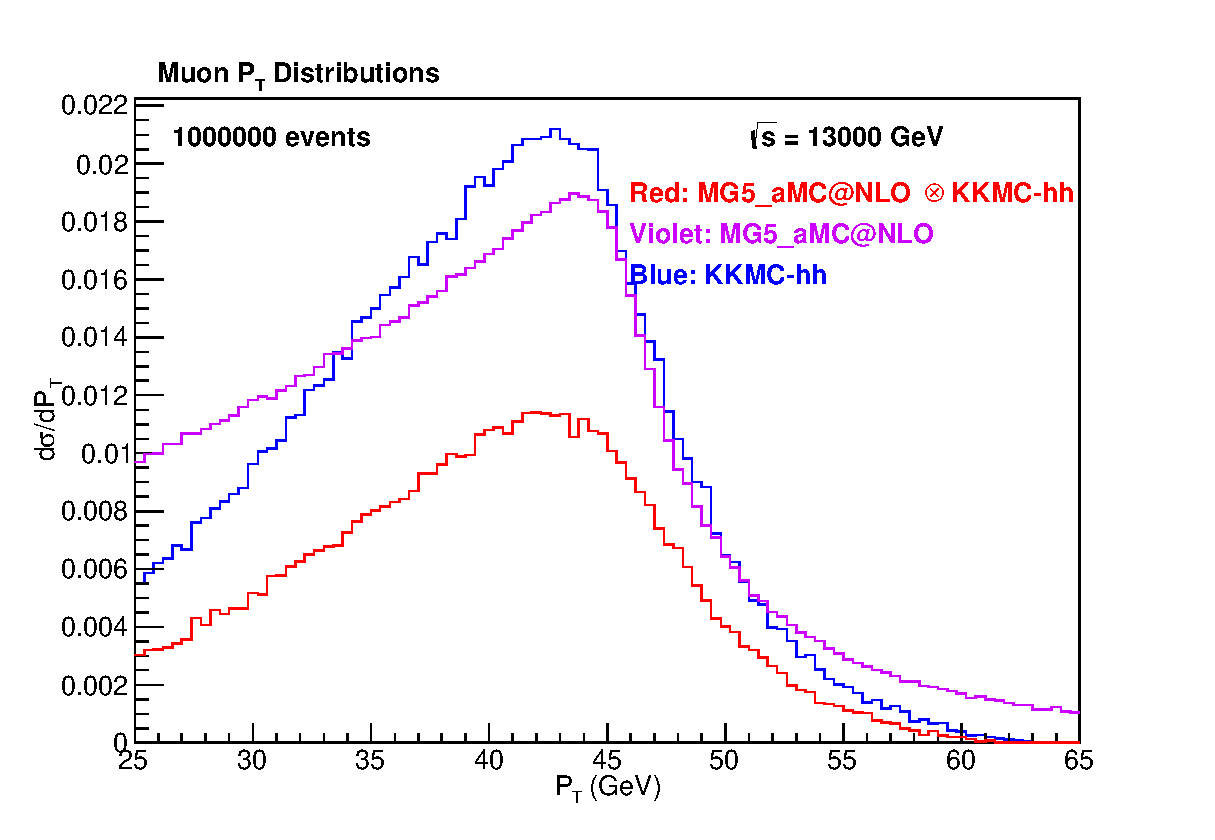
\includegraphics[scale=0.65]{PTL.eps}
		\caption{ Muon transverse momentum distributions for KKMC-hh (blue), MG5\textunderscore aMC@NLO (violet) and MG5\textunderscore aMC@NLO interfaced with KKMC-hh (red) with the cuts specified in the text. }
	\end{center}
\end{figure}

The next quantity we compared is the muon pseudorapidity distribution. The pseudorapidity $\eta$ is a spatial coordinate describing the angle of a particle relative to the beam axis, commonly used in the experimental particle physics. It is defined as 
\begin{equation}
\eta=\log\left(\tan\frac{\theta}{2}\right),
\end{equation} 
where the angle $\theta$ is angle between the particle three-momentum $\vec{p}$ and the positive direction of the beam axis. The pseudorapidity can also be expressed in terms of three-momentum:
\begin{equation}
\eta\equiv\frac{1}{2}\log\left(\frac{|p|+p_L}{|p|-p_L}\right),
\end{equation}
where $p_L$ is the component of the momentum along the beam axis, namely, the longitudinal momentum. From Figure 8.2, we find that interfacing MG5\textunderscore aMC@\newline
NLO with KKMC-hh results an apparent enhancement on the muon pseudorapidity distribution compared with that derived from MG5\textunderscore aMC@NLO.
\begin{figure}
	\begin{center}
		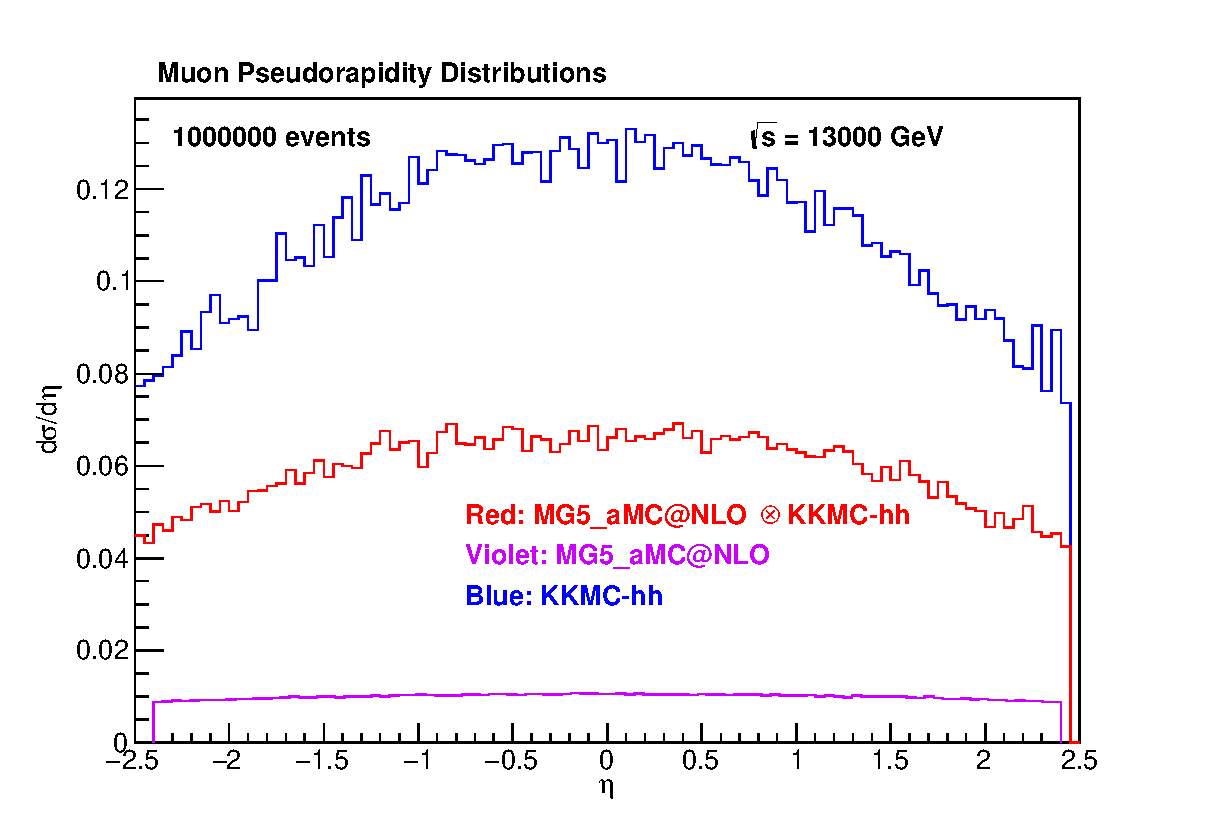
\includegraphics[scale=0.65]{ETA.eps}
		\caption{ Muon pseudorapidity distributions for KKMC-hh (blue), MG5\textunderscore aMC@NLO (violet) and MG5\textunderscore aMC@NLO interfaced with KKMC-hh (red) with the cuts specified in the text. }
	\end{center}
	\end{figure}

We compared not only quantities of the single lepton but those of lepton pairs as well. The dimuon transverse momentum distributions obtained by these three approaches are given in the Figure 8.3. As we can see, the differential cross section calculated by MG5\textunderscore aMC@NLO interfaced with KKMC-hh is larger than that obtained by MG5\textunderscore aMC@NLO only, and the enhancement is from the EW corrections calculated by KKMC-hh. 

And the Figure 8.4 described the dimuon invariant mass distributions. By comparing the dimuon invariant mass distribution derived from MG5\textunderscore aMC@NLO interfaced with KKMC-hh with that from MG5\textunderscore aMC@NLO only, we find there is also an enhancement that is due to the EW corrections provided by KKMC-hh. Besides, we see the resonance peaks near $91\text{ GeV}$ derived from these three generators.
\begin{figure}
	\begin{center}
		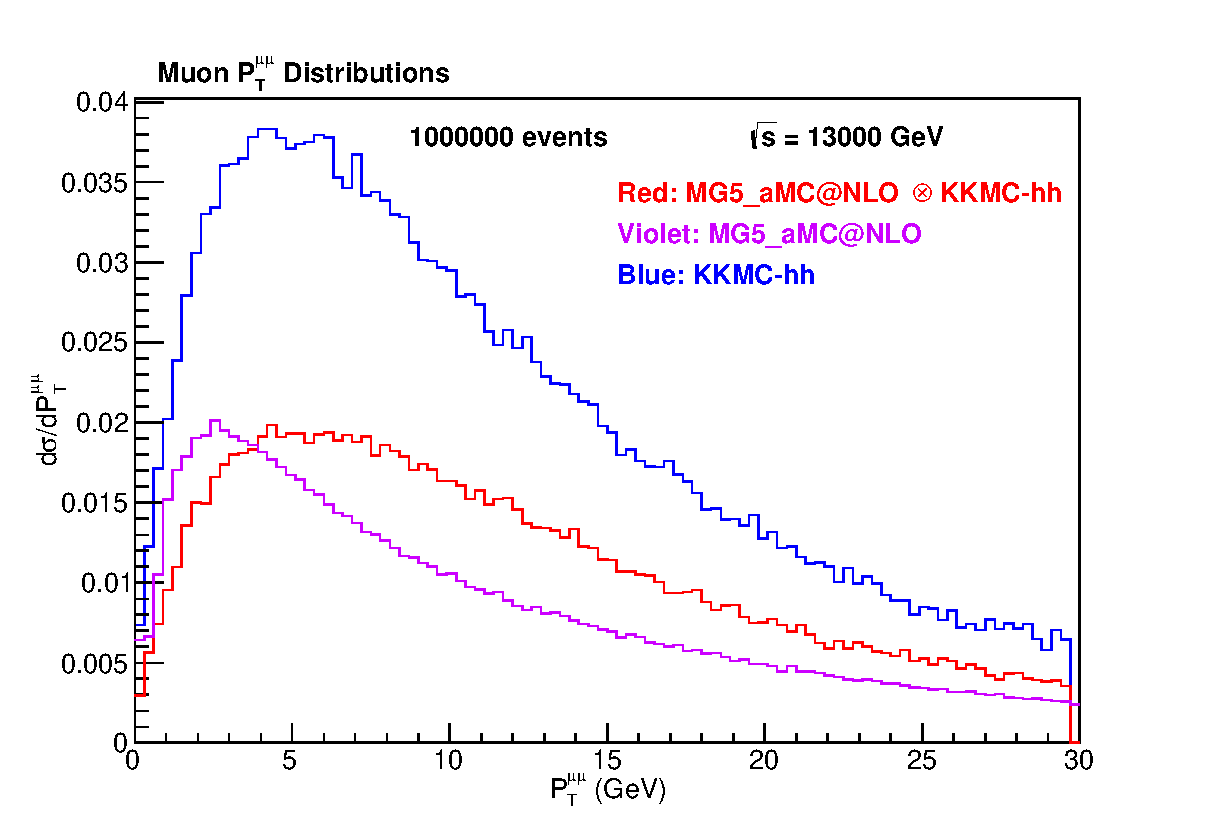
\includegraphics[scale=0.65]{PTLL.eps}
		\caption{ Dimuon transverse momentum distributions for KKMC-hh (blue), MG5\textunderscore aMC@NLO (violet) and MG5\textunderscore aMC@NLO interfaced with KKMC-hh (red) with the cuts specified in the text.  }
	\end{center}
\end{figure}

Finally, let us see the dimuon rapidity distributions in the Figure 8.5. The rapidity is defined as 
\begin{equation}
y\equiv\frac{1}{2}\log\left(\frac{E+p_L}{E-p_L}\right).
\end{equation}
We see that MG5\textunderscore aMC@NLO interfaced with KKMC-hh amplified the dimuon rapidity distribution obtained by MG5\textunderscore aMC@NLO only. The amplification can be viewed as a consequence of the EW corrections.


\begin{figure}
	\begin{center}
		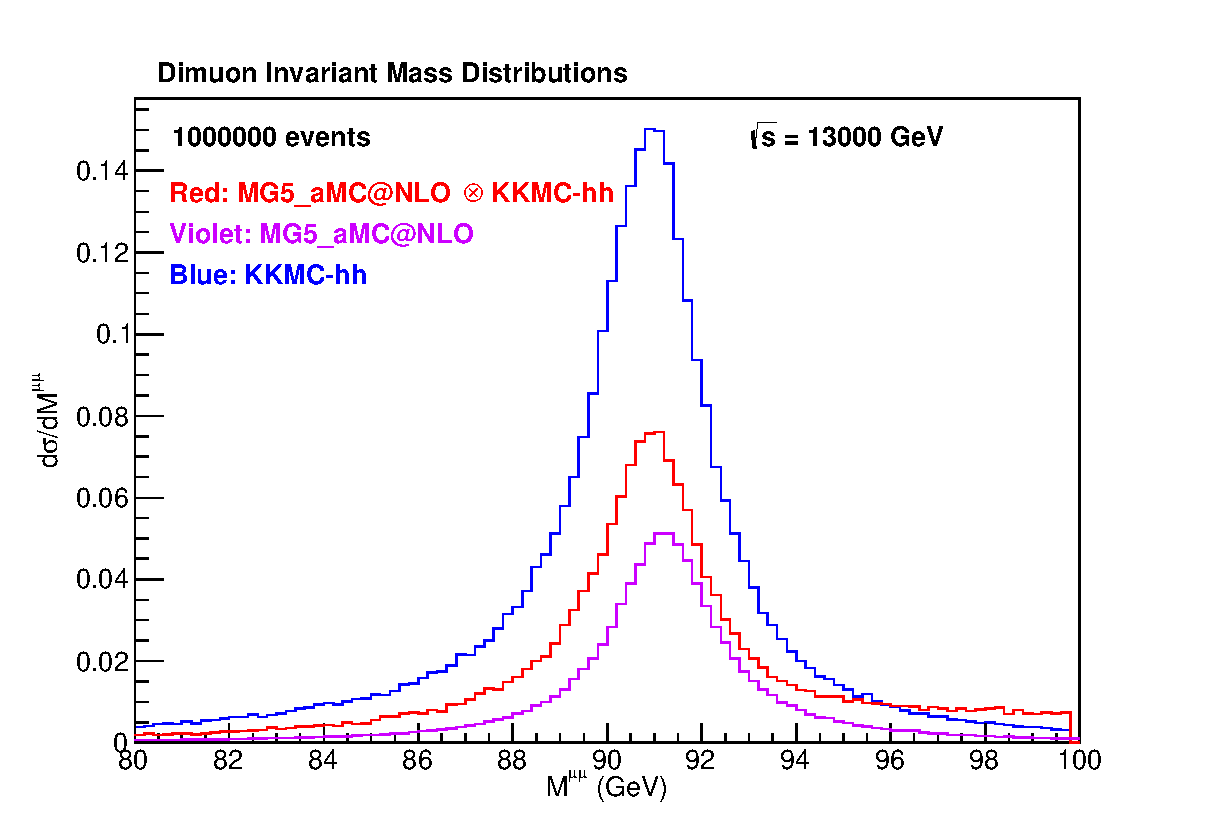
\includegraphics[scale=0.65]{MLL.eps}
		\caption{ Dimuon invariant mass distributions for KKMC-hh (blue), MG5\textunderscore aMC@NLO (violet) and MG5\textunderscore aMC@NLO interfaced with KKMC-hh (red) with the cuts specified in the text. }
	\end{center}
\end{figure} 

In sum, we exhibited the comparisons of the results obtained by MG5\textunderscore aMC@\newline NLO$\otimes$KKMC-hh, MG5\textunderscore aMC@NLO and KKMC-hh. We find that MG5\textunderscore aMC@NLO interfaced with KKMC-hh would enhance the results obtained by MG5\textunderscore aMC@NLO only and the enhancement is due to the EW corrections derived from KKMC-hh.

\begin{figure}
	\begin{center}
		\includegraphics[scale=0.65]{Y.eps}
		\caption{ Dimuon radipity distributions for KKMC-hh (blue), MG5\textunderscore aMC@NLO (violet) and MG5\textunderscore aMC@NLO interfaced with KKMC-hh (red) with the cuts specified in the text. }
	\end{center}
\end{figure}
\include{Overall-Summary}

% Appendices (optional)
\multipleappendices % Change to \multipleappendices if you have more than one!
\begin{appendices}
	\chapter{Feynman Rules of the Electroweak SM} 

In this appendix we outline the Feynman rules of electroweak SM in the 't Hooft-Feynman gauge including the counterterms. In the verticles all momenta are set up as incoming. 

	
Propagators:

for gauge bosons $V=\gamma, Z, W$ in the 't Hooft-Feynamn gauge($\xi_i=1$)	

\begin{axopicture}(260,60) %vector boson
	\Photon(20,30)(110,30){3}{6.5}
	\Vertex(20,30){1}
	\Vertex(110,30){1}
	\Text(10,30){$V_\mu$}\Text(120,30){$V_\nu$}\Text(60,40){$k$}
	\Text(170,30){$=\frac{-ig_{\mu\nu}}{k^2-M_V^2}$,}	
\end{axopicture}

for Faddeev-Popov ghosts $G=u^\gamma,u^Z,u^W$

\begin{axopicture}(260,60) %ghost
	\DashLine[arrow](20,30)(110,30){2}
	\Vertex(20,30){1}
	\Vertex(110,30){1}
	\Text(10,30){$G$}\Text(120,30){$\bar{G}$}\Text(60,40){$k$}
	\Text(170,30){$=\frac{i}{k^2-M_G^2}$,}	
\end{axopicture}

for scalar fields $S=H,\chi,\phi$

\begin{axopicture}(260,60) %scalar
	\DashLine[arrow](20,30)(110,30){10}
	\Vertex(20,30){1}
	\Vertex(110,30){1}
	\Text(10,30){$S$}\Text(120,30){${S}$}\Text(60,40){$k$}
	\Text(170,30){$=\frac{i}{k^2-M_S^2}$,}	
\end{axopicture}

and for fermion fields $F=f_i$

\begin{axopicture}(260,60)
	\Line[arrow](20,30)(110,30)
	\Vertex(20,30){1}
	\Vertex(110,30){1}
	\Text(10,30){$F$}\Text(120,30){$\bar{F}$}\Text(60,40){$p$}
	\Text(170,30){$=\frac{i}{\slashed{p}-m_f}$.}	
\end{axopicture}

In the 't Hooft-Feynman gauge we have the following relations:
\begin{equation}
M_{u^\gamma}=0, \quad M_{u^Z}=M_\chi=M_Z, \quad M_{u^\pm}=M_\phi=M_W.
\end{equation}

Tadpole:

\begin{axopicture}(260,60)
	\Line(20,30)(110,30)
	\GCirc(20,30){5.66}{1}	
	\Line(24,26)(16,34)
	\Line(16,26)(24,34)
	\Text(90,40){$S$}
	\Text(170,30){$=i\delta t$.}
\end{axopicture}

$VV$-counterterm:

\begin{axopicture}(260,60) %vector boson
	\Photon(20,30)(110,30){3}{6.5}
	\Vertex(20,30){1}
	\Vertex(110,30){1}
	\Text(10,30){$V_\mu$}\Text(120,30){$V_\nu$}\Text(60,40){$k$}
	\Text(170,30){$=-ig_{\mu\nu}[C_1 k^2-C_2]$}
	\GCirc(65,30){5.66}{1}	
	\Line(61,26)(69,34)
	\Line(69,26)(61,34)	 %counterterm
	
\end{axopicture}
\newline with the actual values of $V_1$, $V_2$ and $C_1$, $C_2$
\begin{eqnarray}
W^+W^-:&& C_1=\delta Z_W, \quad C_2=M_W^2\delta Z_W+\delta M_W^2\nonumber\\
ZZ:&&  C_1=\delta Z_{ZZ}, \quad C_2=M_Z^2\delta Z_{ZZ}+\delta M_Z^2\nonumber\\
AZ:&&  C_1=\frac{1}{2}\delta Z_{AZ}+\frac{1}{2}\delta Z_{ZA}, \quad C_2=M_Z^2\frac{1}{2}\delta Z_{ZA}\nonumber\\
AA:&& C_1=\delta Z_{AA}, \quad C_2=0.
\end{eqnarray}

$SS$-counterterm:

\begin{axopicture}(260,60) %scalar
	\DashLine(20,30)(110,30){10}
	\Vertex(20,30){1}
	\Vertex(110,30){1}
	\Text(10,30){$S_1$}\Text(120,30){${S_2}$}\Text(60,40){$k$}
	\Text(170,30){$=i[C_1 k^2-C_2]$,}
	\GCirc(65,30){5.66}{1}		
	\Line(61,26)(69,34)
	\Line(69,26)(61,34)	 %counterterm
	
\end{axopicture}
\newline with the actual values of $S_1$, $S_2$ and $C_1$, $C_2$
\begin{eqnarray}
HH:C_1=\delta Z_H,\quad C_2=M_H^2\delta Z_H+\delta M_H^2.
\end{eqnarray}

$FF$-counterterm:

\begin{axopicture}(260,60) %fermion
	\Line(20,30)(110,30)
	\Vertex(20,30){1}
	\Vertex(110,30){1}
	\Text(10,30){$F_1$}\Text(120,30){$\bar{F_2}$}\Text(50,40){$p$}
	\Text(170,10){$=i[C_L\slashed{p}\frac{1}{2}(1-\gamma_5)+C_R\slashed{p}\frac{1}{2}(1+\gamma_5)]-C_S^-\slashed{p}\frac{1}{2}(1-\gamma_5-C_S^+\slashed{p}\frac{1}{2}(1+\gamma_5)]$,}
	\GCirc(65,30){5.66}{1}	
	\Line(61,26)(69,34)
	\Line(69,26)(61,34)	 %counterterm
	
\end{axopicture}
\newline with the actual values of $F_1$, $\bar{F}_2$ and $C_L, C_R, C_S^-, C_S^+$
\begin{equation}
f_i\bar{f}_i:\begin{cases} 
C_L=\frac{1}{2}(\delta Z^{f,L}_{ij}+\delta Z^{f,L,\dagger}_{ij}),
\\ C_R=\frac{1}{2}(\delta Z^{f,R}_{ij}+\delta Z^{f,R,\dagger}_{ij})
\\
C^-_S=m_{f,i}\frac{1}{2}\delta Z^{f,L}_{ij}+m_{f,i}\frac{1}{2}\delta Z^{f,R,\dagger}_{ij}+\delta_{ij}\delta m_{f,i},\\
C^+_S=m_{f,i}\frac{1}{2}\delta Z^{f,R}_{ij}+m_{f,i}\frac{1}{2}\delta Z^{f,L,\dagger}_{ij}+\delta_{ij}\delta m_{f,i}.
\end{cases}
\end{equation}


$VVVV$-couping:

\begin{axopicture}(260,130) %fermion
	\Photon(20,110)(65,65){3}{5.5}
	\Photon(65,65)(110,20){3}{5.5}
	\Photon(20,20)(65,65){3}{5.5}
	\Photon(65,65)(110,110){3}{5.5}
	\Vertex(65,65){1}		
	\Text(10,110){$V_{1,\mu}$}
	\Text(10,10){$V_{2,\nu}$}
	\Text(120,10){$V_{4,\sigma}$}
	\Text(120,110){$V_{3,\rho}$}
	\Text(210, 65){$=ie^2C[2g_{\mu\nu}g_{\sigma\rho}-g_{\nu\rho}g_{\mu\sigma}-g_{\rho\mu}g_{\nu\sigma}]$}
	\Vertex(65,65){3}
\end{axopicture}
\newline with the actual values of $V_1$,$V_2$,$V_3$,$V_4$ and $C$
\begin{eqnarray}
W^+W^+W^-W^-:&& C=\frac{1}{s_W^2}\left[1+2\delta Z_e-2\frac{\delta s_W}{s_W}+2\delta Z_W\right]\nonumber\\
W^+W^-ZZ:&& C=-\frac{c_W^2}{s_W^2}\left[1+2\delta Z_e-2\frac{1}{c^2}\frac{\delta s_W}{s_W}+2\delta Z_W+\frac{1}{2}\delta Z_ZZ\right]+\frac{1}{2}\frac{c_W}{s_W}\nonumber\\
W^+W^-AZ:&&C=
\frac{c_W}{s_W}\left[1+2\delta Z_e-\frac{1}{c^2}\frac{\delta s_W}{s_W}+\delta Z_W+\frac{1}{2}\delta Z_{ZZ}+\frac{1}{2}\delta Z_{AA}\right]\nonumber\\
&&-\frac{1}{2}\delta Z_{AZ}
-\frac{1}{2}\frac{c^2_W}{s^2_W}\delta Z_{ZA}\nonumber\\
W^+W^-AA:&&C=-\left[1+2\delta Z_e+\delta Z_W+\delta Z_{AA}\right]+\frac{1}{2}\frac{c_W}{s_W}\delta Z_{ZA}.
\end{eqnarray}

$VVV$-couping:

\begin{axopicture}(260,130) %fermion
	\Photon(10,65)(65,65){3}{5.5} 
	\Photon(65,65)(120,35){3}{5.5}
	\Photon(65,65)(120,105){3}{5.5}
	\Vertex(65,65){1}		
	\Text(10,75){$V_{1,\mu}, k_1$}
	\Text(110,20){$V_{3,\rho},k_3$}
	\Text(110,110){$V_{2,\nu},k_2$}
	\Text(220, 65){$=-ieC[g_{\mu\nu}(k_2-k_1)_\rho-g_{\nu\rho}(k_3-k_2)_\mu$}
	\Text(175,50){$-g_{\rho\mu}(k_1-k_3)_\nu$}
	\Vertex(65,65){3}
\end{axopicture}
\newline with the actual values of $V_1$,$V_2$,$V_3$ and $C$
\begin{eqnarray}
AW^+W^-:&&C=1+\delta Z_e+\delta Z_W+\frac{1}{2}\delta Z_{AA}-\frac{1}{2}\frac{c_W}{s_W}\delta Z_{ZA},\nonumber\\
ZW^+W^-:&&C=-\frac{c_W}{s_W}\left[1+\delta Z_e-\frac{1}{c^2}\frac{\delta s_W}{s_W}+\delta Z_W+\frac{1}{2}\delta Z_{ZZ}\right]+\frac{1}{2}\delta Z_{AZ}.\nonumber\\
\end{eqnarray}

$SSSS$-couping:

\begin{axopicture}(260,130) %fermion
	\Line[dash](20,110)(65,65)
	\Line[dash](65,65)(110,20)
	\Line[dash](20,20)(65,65)
	\Line[dash](65,65)(110,110)
	\Vertex(65,65){1}		
	\Text(10,110){$S_{1}$}
	\Text(10,10){$S_{2}$}
	\Text(120,10){$S_{4,}$}
	\Text(120,110){$S_{3}$}
	\Text(160, 65){$=ie^2C$}
	\Vertex(65,65){3}
\end{axopicture}
\newline with the actual values of $S_1$,$S_2$,$S_3$,$S_4$ and $C$
\begin{eqnarray}
HHHH:&& C=-\frac{3}{4s_W^2}\frac{M^2_H}{M^2_W}\left[1+2\delta Z_e-2\frac{\delta s_W}{s_W}+\frac{\delta M^2_H}{M^2_H}-\frac{\delta M^2_H}{M^2_H}+2\delta Z_H\right],\nonumber\\
HH\chi\chi:&& C=-\frac{1}{4s_W^2}\frac{M^2_H}{M^2_W}\left[1+2\delta Z_e-2\frac{\delta s_W}{s_W}+\frac{\delta M^2_H}{M^2_H}-\frac{\delta M^2_H}{M^2_H}+\delta Z_H\right],\nonumber\\
HH\phi\phi:&& C=-\frac{1}{4s_W^2}\frac{M^2_H}{M^2_W}\left[1+2\delta Z_e-2\frac{\delta s_W}{s_W}+\frac{\delta M^2_H}{M^2_H}-\frac{\delta M^2_H}{M^2_H}+\delta Z_H\right],\nonumber\\
\chi\chi\chi\chi:&& C=-\frac{3}{4s_W^2}\frac{M^2_H}{M^2_W}\left[1+2\delta Z_e-2\frac{\delta s_W}{s_W}+\frac{\delta M^2_H}{M^2_H}-\frac{\delta M^2_H}{M^2_H}\right],\nonumber\\
\chi\chi\phi\phi:&& C=-\frac{1}{4s_W^2}\frac{M^2_H}{M^2_W}\left[1+2\delta Z_e-2\frac{\delta s_W}{s_W}+\frac{\delta M^2_H}{M^2_H}-\frac{\delta M^2_H}{M^2_H}\right],\nonumber\\
\phi\phi\phi\phi:&& C=-\frac{1}{2s_W^2}\frac{M^2_H}{M^2_W}\left[1+2\delta Z_e-2\frac{\delta s_W}{s_W}+\frac{\delta M^2_H}{M^2_H}-\frac{\delta M^2_H}{M^2_H}\right].\nonumber\\
\end{eqnarray}

$SSS$-couping:

\begin{axopicture}(260,130) %fermion
	\Line[dash](10,65)(65,65)
	\Line[dash](65,65)(120,35)
	\Line[dash](65,65)(120,105)
	\Vertex(65,65){1}		
	\Text(10,75){$S_1$}
	\Text(110,25){$S_3$}
	\Text(110,110){$S_2$}
	\Text(160, 65){$=ieC$}
	\Vertex(65,65){3}
\end{axopicture}
\newline with the actual values of $S_1$,$S_2$,$S_3$ and $C$
\begin{eqnarray}
HHH:&&C=-\frac{3}{2s}\frac{M^2_H}{m_W}\left[ 1+\delta Z_e-\frac{\delta s_W}{s_W}+\frac{\delta M^2_H}{M^2_H}-\frac{1}{2}\frac{\delta M^2_W}{M^2_W}+\frac{3}{2}\delta Z_H \right],\nonumber\\
H\chi\chi:&&C=-\frac{1}{2s}\frac{M^2_H}{m_W}\left[ 1+\delta Z_e-\frac{\delta s_W}{s_W}+\frac{\delta M^2_H}{M^2_H}-\frac{1}{2}\frac{\delta M^2_W}{M^2_W}+\frac{1}{2}\delta Z_H \right],\nonumber\\
H\chi\chi:&&C=-\frac{1}{2s}\frac{M^2_H}{m_W}\left[ 1+\delta Z_e-\frac{\delta s_W}{s_W}+\frac{\delta M^2_H}{M^2_H}-\frac{1}{2}\frac{\delta M^2_W}{M^2_W}+\frac{1}{2}\delta Z_H \right].\nonumber\\
\end{eqnarray}


$VVVV$-couping:

\begin{axopicture}(260,130) %fermion
	\Photon(20,110)(65,65){3}{5.5}
	\Line[dash](65,65)(110,20)
	\Photon(20,20)(65,65){3}{5.5}
	\Line[dash](65,65)(110,110)
	\Vertex(65,65){1}		
	\Text(10,110){$V_{1,\mu}$}
	\Text(10,10){$V_{2,\nu}$}
	\Text(120,10){$S_2$}
	\Text(120,110){$S_1$}
	\Text(170, 65){$=ie^2g_{\mu\nu}C$}
	\Vertex(65,65){3}
\end{axopicture}
\newline with the actual values of $V_1$,$V_2$,$S_1$,$S_2$ and $C$
\begin{eqnarray*}
	W^+W^-HH:&&C=\frac{1}{2s^2}\left[ 1+2\delta Z_e-2\frac{\delta s_W}{s_W}+\delta Z_W+\delta Z_H \right],\nonumber\\
	W^+W^-\chi\chi:&&C=\frac{1}{2s^2}\left[ 1+2\delta Z_e-2\frac{\delta s_W}{s_W}+\delta Z_W \right],\nonumber\\
	W^+W^-\phi\phi:&&C=\frac{1}{2s^2}\left[ 1+2\delta Z_e-2\frac{\delta s_W}{s_W}+\delta Z_W \right],\nonumber\\
	ZZ\phi^+\phi^-:&&C=\frac{s^2_W-c^2_W}{2s_W^2c_W^2}\left[ 1+2\delta Z_e+\frac{2}{(s_W^2-c_W^2)c^2_W}\frac{\delta s_W}{s_W}+\delta Z_{ZZ} \right]\nonumber\\
	&&+\frac{s^2_W-c^2_W}{s_Wc_W}\frac{1}{2}\delta Z_{AZ},\nonumber\\
	ZA\phi^+\phi^-:&&C=\frac{s^2_W-c^2_W}{2s_W^2c_W^2}\biggl[ 1+2\delta Z_e+\frac{1}{(s_W^2-c_W^2)c^2_W}\frac{\delta s_W}{s_W}+\frac{1}{2}\delta Z_{ZZ} \nonumber\\
	&&+\frac{1}{2}Z_{AA}\biggr]+\frac{1}{2}\frac{(s_W^2-c_W^2)^2}{2s^2_Wc^2_W}\delta Z_{ZA}+\delta Z_{AZ},\nonumber\\
	AA\phi^+\phi^-:&& C=2[1+2\delta Z_e+\delta Z_{AA}]+\frac{1}{2}\frac{s^2_W-c^2_W}{s_Wc_W}\delta Z_{ZA},\nonumber\\
	ZZHH:&&C=\frac{1}{2s^2_Wc^2_W}\biggl[ 1+2\delta Z_e+2\frac{s^2_W-c^2_W}{c^2_W}\frac{\delta s_W}{s_W}+\delta ZZ+\delta Z_H \biggr],\nonumber\\
	ZZ\chi\chi:&&=\frac{1}{2s^2_Wc^2_W}\biggl[ 1+2\delta Z_e+2\frac{s^2_W-c^2_W}{c^2_W}\frac{\delta s_W}{s_W}+\delta ZZ \biggr],\nonumber\\
	ZAHH:&& C=\frac{1}{2s^2_Wc^2_W}\frac{1}{2}\delta Z_{ZA},\nonumber\\
	ZA\chi\chi:&& C=\frac{1}{2s^2_Wc^2_W}\frac{1}{2}\delta Z_{ZA},\nonumber\\
\end{eqnarray*}
\begin{eqnarray}
W^\pm Z\phi^\mp H:&& C=-\frac{1}{2c_w}\biggl[ 1+\delta Z_e-\frac{\delta c_W}{c_W}+\frac{1}{2}\delta Z_W+\frac{1}{2}\delta Z_H+\frac{1}{2}\delta Z_{ZZ}\biggr]\nonumber\\
&&-\frac{1}{2}\frac{1}{s_W}\delta Z_{AZ} ,\nonumber\\
W^\pm A\phi^\mp H:&& C=-\frac{1}{2s_w}\biggl[ 1+\delta Z_e-\frac{\delta s_W}{s_W}+\frac{1}{2}\delta Z_W+\frac{1}{2}\delta Z_H+\frac{1}{2}\delta Z_{AA} \biggr]\nonumber\\
&&-\frac{1}{2}\frac{1}{c_W}\delta Z_{ZA},\nonumber\\
W^\pm Z\phi^\mp \chi:&& C=\mp\frac{i}{2c_w}\biggl[ 1+\delta Z_e-\frac{\delta c_W}{c_W}+\frac{1}{2}\delta Z_W+\frac{1}{2}\delta Z_{ZZ} \biggr]\mp\frac{1}{2}\frac{i}{2s_W}\delta Z_{AZ},\nonumber\\
W^\pm Z\phi^\mp \chi:&& C=\mp\frac{i}{2s_w}\biggl[ 1+\delta Z_e-\frac{\delta s_W}{s_W}+\frac{1}{2}\delta Z_W+\frac{1}{2}\delta Z_{AA} \biggr]\mp\frac{1}{2}\frac{i}{2c_W}\delta Z_{ZA}.\nonumber\\
\end{eqnarray}

$VSS$-couping:

\begin{axopicture}(260,130) %fermion
	\Photon(10,65)(65,65){3}{5.5}
	\Line[dash](65,65)(120,35)
	\Line[dash](65,65)(120,105)
	\Vertex(65,65){1}		
	\Text(10,75){$V_\mu$}
	\Text(110,25){$S_2,k_2$}
	\Text(110,110){$S_1,k_1$}
	\Text(180, 65){$=ieC(k_1-k_2)_\mu$}
	\Vertex(65,65){3}
\end{axopicture}
\newline with the actual values of $V$, $S_1$,$S_2$ and $C$
\begin{eqnarray}
A\chi H:&& C=-\frac{1}{2}\frac{i}{2c_Ws_W}\delta Z_{ZA},\nonumber\\
Z\chi H:&& C=-\frac{i}{2c_ws_W}\biggl[ 1+\delta Z_e+\frac{s^2_W-c^2_W}{c^2_W}\frac{\delta s_W}{s_W}+\frac{1}{2}\delta Z_H+\frac{1}{2}\delta Z_{ZZ} \biggr],\nonumber\\
A\phi^+\phi^-:&& C=-\biggl[ 1+\delta Z_e+\frac{1}{2}\delta Z_{AA}+\frac{1}{2}\frac{s^2_W-c^2_W}{2s_Wc_W}\delta Z_{ZA} \biggr],\nonumber\\
Z\phi^+\phi^-:&& C=-\frac{s^2_w-c^2_W}{2s_Wc_W}\biggl[ 1+\delta Z_e+\frac{1}{(s^2_W-c^2_W)c^2_W}\frac{\delta s_w}{s_W}+\frac{1}{2}\delta Z_{ZZ} \biggr]-\frac{1}{2}\delta Z_{AZ},\nonumber\\
W^\pm\phi^\pm H:&& C=\mp\frac{1}{2s_W}\biggl[ 1+\delta Z_e-\frac{\delta s_W}{s_W}+\frac{1}{2}\delta Z_W+\frac{1}{2}\delta Z_H \biggr],\nonumber\\
W^\pm\phi^\pm \chi:&& C=-\frac{i}{2s_W}\biggl[ 1+\delta Z_e-\frac{\delta s_W}{s_W}+\frac{1}{2}\delta Z_W \biggr].\nonumber\\
\end{eqnarray}

$SVV$-couping:

\begin{axopicture}(260,130) %fermion
	\Line[dash](10,65)(65,65)
	\Photon(65,65)(120,35){3}{5.5}
	\Photon(65,65)(120,105){3}{5.5}
	\Vertex(65,65){1}		
	\Text(10,75){$S$}
	\Text(110,25){$V_{2,\rho}$}
	\Text(110,110){$V_{1,\nu}$}
	\Text(170, 65){$=ieg_{\mu\nu}C$}
	\Vertex(65,65){3}
\end{axopicture}
\newline with the actual values of $S$, $V_1$,$V_2$ and $C$
\begin{eqnarray}
HW^+W^-:&& C=M_W\frac{1}{s_W}\biggl[ 1+\delta Z_e-\frac{\delta s_W}{s_W}+\frac{1}{2}\frac{\delta M^2_W}{M_W^2}+\frac{1}{2}\delta Z_H+\delta Z_W \biggr]\nonumber\\
HZZ:&& C=M_W\frac{1}{s_Wc^2_W}\biggl[ 1+\delta Z_e+\frac{2s^2_W-c^2_W}{c^2_W}\frac{\delta s_W}{s_W}+\frac{1}{2}\frac{\delta M^2_W}{M_W^2}+\frac{1}{2}\delta Z_H+\delta Z_{ZZ} \biggr],\nonumber\\
HZA:&& C=M_W\frac{1}{s_Wc^2_W}\frac{1}{2}\delta Z_{ZA},\nonumber\\
\phi^\pm
W^\mp Z:&& C=-M_W\frac{s_W}{c_W}\biggl[ 1+\delta Z_e+\frac{1}{c^2_W}\frac{\delta s_W}{s_W}+\frac{1}{2}\frac{\delta M^2_W}{M_W^2}+\frac{1}{2}\delta Z_W+\frac{1}{2}\delta Z_{ZZ} \biggr],\nonumber\\
\phi^\pm W^\mp A:&& C=-M_W\biggl[ 1+\delta Z_e+\frac{1}{2}\frac{\delta M^2_W}{M_W^2}+\frac{1}{2}\delta Z_W+\frac{1}{2}\delta Z_{AA} \biggr]-M_W\frac{s_W}{c_W}\frac{1}{2}\delta Z_{ZA}.\nonumber\\
\end{eqnarray}

$VFF$-couping:

\begin{axopicture}(260,130) %fermion
	\Photon(10,65)(65,65){3}{5.5}
	\Line[arrow](120,35)(65,65)
	\Line[arrow](65,65)(120,105)
	\Vertex(65,65){1}		
	\Text(10,75){$V_\mu$}
	\Text(110,25){$F_2$}
	\Text(110,110){$\bar{F}_1$}
	\Text(180, 65){$=ie\gamma_{\mu}(C^-\omega_-+C^+\omega_+)$}
	\Vertex(65,65){3}
\end{axopicture}
\newline with the actual values of $V$, $\bar{F}_1$,$F_2$ and $C^+$ and $C^-$
\begin{eqnarray}
\gamma\bar{f}_if_j:&&
\begin{cases}
C^+=-Q_f[ \delta_{ij}( 1+\delta Z_e+\frac{1}{2}\delta Z_{AA})+\frac{1}{2}(\delta Z^{f,R}_{ij}+\delta Z^{f,R\dagger}_{ij})]+\delta_{ij}g^+_f\frac{1}{2}\delta Z_{ZA},\\
C^-=-Q_f[ \delta_{ij}( 1+\delta Z_e+\frac{1}{2}\delta Z_{AA})+\frac{1}{2}(\delta Z^{f,L}_{ij}+\delta Z^{f,L\dagger}_{ij})]+\delta_{ij}g^-_f\frac{1}{2}\delta Z_{ZA},\\
\end{cases}\nonumber\\
Z\bar{f}_if_j:&&
\begin{cases}
C^+=g^+_f[ \delta_{ij}( 1+\frac{\delta g^+_f}{g^+_f}+\frac{1}{2}\delta Z_{ZZ})+\frac{1}{2}(\delta Z^{f,R}_{ij}+\delta Z^{f,R\dagger}_{ij})]-\delta_{ij}Q_f\frac{1}{2}\delta Z_{AZ},\\
C^-=g^+_f[ \delta_{ij}( 1+\frac{\delta g^-_f}{g^-_f}+\frac{1}{2}\delta Z_{ZZ})+\frac{1}{2}(\delta Z^{f,L}_{ij}+\delta Z^{f,L\dagger}_{ij})]-\delta_{ij}Q_f\frac{1}{2}\delta Z_{AZ},\\
\end{cases}\nonumber\\
W^+\bar{u}_id_j:&&
\begin{cases}
C^+=0,\\
C^-=\frac{1}{\sqrt{2}s_W}\biggl[V_{ij}\biggl(1+\delta Z_e-\frac{\delta S_W}{s_W}+\frac{1}{2}\delta Z_W\biggr)+\delta V_{ij}
+\frac{1}{2}\sum_k(\delta Z^{u,L\dagger}_{jk}V_{kj}\\
\quad\quad+V_{ik}\delta Z^{d,L}_{kj})\biggr],
\end{cases}\nonumber\\
W^-\bar{d}_ju_i:&&
\begin{cases}
C^+=0,\\
C^-=\frac{1}{\sqrt{2}s_W}\biggl[V_{ji}^\dagger\biggl(1+\delta Z_e-\frac{\delta S_W}{s_W}+\frac{1}{2}\delta Z_W\biggr)+\delta V_{ji}^\dagger
+\frac{1}{2}\sum_k(\delta Z^{d,L\dagger}_{jk}V_{ki}^\dagger\\
\quad\quad+V_{jk}^\dagger\delta Z^{u,L}_{ki})\biggr],
\end{cases}\nonumber\\
W^+\bar{\nu}_il_j:&&
\begin{cases}
C^+=0,\\
C^-=\frac{1}{\sqrt{2}s_W}\delta_{ij}\biggl[ 1+\delta Z_e-\frac{\delta s_W}{s_W}+\frac{1}{2}\delta Z_W+\frac{1}{2}(\delta Z^{\nu,L\dagger})_{ii}+\delta Z^{l,L}_{ii} \biggr],
\end{cases}\nonumber\\
W^-\bar{l}_j\nu_i:&&
\begin{cases}
C^+=0,\\
C^-=\frac{1}{\sqrt{2}s_W}\delta_{ij}\biggl[ 1+\delta Z_e-\frac{\delta s_W}{s_W}+\frac{1}{2}\delta Z_W+\frac{1}{2}(\delta Z^{l,L\dagger})_{ii}+\delta Z^{\nu,L}_{ii} \biggr],
\end{cases}
\end{eqnarray}
where
\begin{eqnarray}
&g^+_f=-\frac{s_W0}{c_W}Q_f,&\delta g^+_f=-\frac{s_W}{c_W}Q_f\biggl[ \delta Z_e+\frac{1}{c_W^2}\frac{\delta s_W}{s_W} \biggr],\nonumber\\
&g^-_f=\frac{I^3_{W,f}-s^2_WQ_f}{s_Wc_W},&\delta g^+_f=\frac{I^2_{W,f}}{s_Wc_W}Q_f\biggl[ \delta Z_e+\frac{s^2_W-c^2_W}{c_W^2}\frac{\delta s_W}{s_W} \biggr]+\delta g^+_f.
\end{eqnarray}
The vector and axial vector couplings fo the $Z$-boson are given by
\begin{equation}
v_f=\frac{1}{2}(g^-+g^+)=\frac{I^3_{W,f}-2s_W^2Q_f}{2s_Wc_W},\quad a_f=\frac{1}{2}(g^-_f-g^+_f)=\frac{I^3_{W,f}}{2s_Wc_W}.
\end{equation}
\newpage
$SFF$-couping:

\begin{axopicture}(260,130) %fermion
	\Line[dash](10,65)(65,65)
	\Line[arrow](120,35)(65,65)
	\Line[arrow](65,65)(120,105)
	\Vertex(65,65){1}		
	\Text(10,75){$V_\mu$}
	\Text(110,25){$F_2$}
	\Text(110,110){$\bar{F}_1$}
	\Text(180, 65){$=ie(C^-\omega_-+C^+\omega_+)$}
	\Vertex(65,65){3}
\end{axopicture}
\newline with the actual values of $S$, $\bar{F}_1$,$F_2$ and $C^+$ and $C^-$
\begin{eqnarray*}
	H\bar{f}_if_j:&&\begin{cases}
		C^+=-\frac{1}{2s_W}\frac{m_{f,i}}{M_W}\biggl[ \delta_{ij}\biggl(  1+\delta Z_e-\frac{\delta s_w}{s_W}+\frac{\delta m_{f,i}}{m_{f,i}}-\frac{\delta M_W}{M_W}+\frac{1}{2}\delta Z_H \biggr)\\
		\quad\quad\quad+\frac{1}{2}(\delta Z^{f,R}_{ij}+\delta Z^{f,R\dagger}_{ij}) \biggr],\\
		C^-=-\frac{1}{2s_W}\frac{m_{f,i}}{M_W}\biggl[ \delta_{ij}\biggl(  1+\delta Z_e-\frac{\delta s_w}{s_W}+\frac{\delta m_{f,i}}{m_{f,i}}-\frac{\delta M_W}{M_W}+\frac{1}{2}\delta Z_H \biggr)\\
		\quad\quad\quad+\frac{1}{2}(\delta Z^{f,L}_{ij}+\delta Z^{f,L\dagger}_{ij}) \biggr],
	\end{cases}\nonumber\\
	\chi\bar{f}_if_j:&&\begin{cases}
		C^+=i\frac{1}{2s_W}2I^3_{W,f}\frac{m_{f,i}}{M_W}\biggl[ \delta_{ij}\biggl(  1+\delta Z_e-\frac{\delta s_w}{s_W}+\frac{\delta m_{f,i}}{m_{f,i}}-\frac{\delta M_W}{M_W} \biggr)\\
		\quad\quad\quad+\frac{1}{2}(\delta Z^{f,R}_{ij}+\delta Z^{f,R\dagger}_{ij}) \biggr],\\
		C^-=-i\frac{1}{2s_W}2I^3_{W,f}\frac{m_{f,i}}{M_W}\biggl[ \delta_{ij}\biggl(  1+\delta Z_e-\frac{\delta s_w}{s_W}+\frac{\delta m_{f,i}}{m_{f,i}}-\frac{\delta M_W}{M_W} \biggr)\\
		\quad\quad\quad+\frac{1}{2}(\delta Z^{f,L}_{ij}+\delta Z^{f,L\dagger}_{ij}) \biggr],
	\end{cases}\nonumber\\
	\phi^+\bar{u}_id_j:&&
	\begin{cases}
		C^+=-\frac{1}{\sqrt{2}s_W}\frac{m_{d,j}}{M_W}\biggl[ V_{ij}\biggl( 1+\delta Z_e-\frac{\delta s_W}{s_W}+\frac{\delta m_{d,j}}{m_{d,j}}-\frac{\delta M_W}{M_W}+\delta V_{ij}\\
		\quad\quad\quad +\frac{1}{2}\sum_k(\delta Z^{u,R\dagger}_{ik}V_{kj}+V_{ik}\delta Z^{d,R}_{kj}) \biggr) \biggr],\\
		C^-=\frac{1}{\sqrt{2}s_W}\frac{m_{u,j}}{M_W}\biggl[ V_{ij}\biggl( 1+\delta Z_e-\frac{\delta s_W}{s_W}+\frac{\delta m_{u,j}}{m_{u,j}}-\frac{\delta M_W}{M_W}+\delta V_{ij}\\
		\quad\quad\quad +\frac{1}{2}\sum_k(\delta Z^{u,L\dagger}_{ik}V_{kj}+V_{ik}\delta Z^{d,L}_{kj}) \biggr) \biggr],\\
	\end{cases}\nonumber\\
\end{eqnarray*}
\begin{eqnarray}
\phi^-\bar{d}_ju_i:&&
\begin{cases}
C^+=\frac{1}{\sqrt{2}s_W}\frac{m_{u,i}}{M_W}\biggl[ V^\dagger_{ji}\biggl( 1+\delta Z_e-\frac{\delta s_W}{s_W}+\frac{\delta m_{u,j}}{m_{u,j}}-\frac{\delta M_W}{M_W}+\delta V_{ji}^\dagger\\
\quad\quad\quad +\frac{1}{2}\sum_k(\delta Z^{d,R\dagger}_{jk}V_{ki}^\dagger+V_{jk}^\dagger\delta Z^{u,R}_{ki}) \biggr) \biggr],\\
C^-=-\frac{1}{\sqrt{2}s_W}\frac{m_{d,i}}{M_W}\biggl[ V^\dagger_{ji}\biggl( 1+\delta Z_e-\frac{\delta s_W}{s_W}+\frac{\delta m_{d,j}}{m_{d,j}}-\frac{\delta M_W}{M_W}+\delta V_{ji}^\dagger\\
\quad\quad\quad +\frac{1}{2}\sum_k(\delta Z^{d,L\dagger}_{jk}V_{ki}^\dagger+V_{jk}^\dagger\delta Z^{u,L}_{ki}) \biggr) \biggr],\\
\end{cases}\nonumber\\
\phi^+\bar{\nu}_il_j:&&
\begin{cases}
C^+=-\frac{1}{\sqrt{2}s_W}\frac{m_{i,j}}{M_W}\delta_{ij}\biggl[  1+\delta Z_e-\frac{\delta s_W}{s_W}+\frac{\delta m_{i,j}}{m_{i,j}}-\frac{\delta M_W}{M_W} +\frac{1}{2}\biggl(\delta Z^{\nu,R\dagger}_{ii}+\delta Z^{l,R}_{ii}  \biggr) \biggr],\\
C^-=0,
\end{cases}\nonumber\\
\phi^-\bar{l}_j\nu_i:&&
\begin{cases}
C^+=0,\\
C^-=-\frac{1}{\sqrt{2}s_W}\frac{m_{i,j}}{M_W}\delta_{ij}\biggl[  1+\delta Z_e-\frac{\delta s_W}{s_W}+\frac{\delta m_{i,j}}{m_{i,j}}-\frac{\delta M_W}{M_W} +\frac{1}{2}\biggl(\delta Z^{l,L\dagger}_{ii}+\delta Z^{\nu,L}_{ii}  \biggr) \biggr].
\end{cases}\nonumber\\
\end{eqnarray}

$VGG$-couping:

\begin{axopicture}(260,130) %fermion
	\Photon(10,65)(65,65){3}{5.5}
	\Line[arrow,dash](120,35)(65,65)
	\Line[arrow,dash](65,65)(120,105)
	\Vertex(65,65){1}		
	\Text(10,75){$V_\mu$}
	\Text(110,25){$G_2,k_2$}
	\Text(110,110){$\bar{G}_1,k_1$}
	\Text(180, 65){$=iek_{1,\mu}C$}
	\Vertex(65,65){3}
\end{axopicture}
\newline with the actual values of $V$, $\bar{G}_1$,$G_2$ and $C$
\begin{eqnarray}
A\bar{u}^\pm u^\pm:&& C=\pm\biggl[1+\delta Z_e+\frac{1}{2}\delta Z_{AA}\biggr]\mp\frac{c_W}{s_W}\frac{1}{2}\delta Z_{AA},\nonumber\\
Z\bar{u}^\pm u^\pm:&& C=\mp\biggl[1+\delta Z_e-\frac{1}{c_W^2}\frac{\delta s_W}{s_W}+\frac{1}{2}\delta Z_{ZZ}\biggr]\pm\frac{1}{2}\delta Z_{AZ},\nonumber\\
W^\pm\bar{u}^\pm u^Z:&& C=\pm\biggl[1+\delta Z_e-\frac{1}{c_W^2}\frac{\delta s_W}{s_W}+\frac{1}{2}\delta Z_{W}\biggr],\nonumber\\
W^\pm\bar{u}^Z u^\mp:&& C=\mp\biggl[1+\delta Z_e-\frac{1}{c_W^2}\frac{\delta s_W}{s_W}+\frac{1}{2}\delta Z_{W}\biggr],\nonumber\\
W^\pm\bar{u}^\pm u^\gamma:&& C=\mp\biggl[1+\delta Z_e+\frac{1}{2}\delta Z_{W}\biggr],\nonumber\\
W^\pm\bar{u}^\gamma u^\pm:&& C=\pm\biggl[1+\delta Z_e+\frac{1}{2}\delta Z_{W}\biggr].
\end{eqnarray}

$SGG$-couping:

\begin{axopicture}(260,130) %fermion
	\Photon(10,65)(65,65){3}{5.5}
	\Line[arrow,dash](120,35)(65,65)
	\Line[arrow,dash](65,65)(120,105)
	\Vertex(65,65){1}		
	\Text(10,75){$V_\mu$}
	\Text(110,25){$G_2$}
	\Text(110,110){$\bar{G}_1$}
	\Text(180, 65){$=ieC$}
	\Vertex(65,65){3}
\end{axopicture}
\newline with the actual values of $S$, $\bar{G}_1$,$G_2$ and $C$
\begin{eqnarray}
H\bar{u}^Zu^Z:&&C=-\frac{1}{2s_Wc_W^2}M_W\biggl[ 1+\delta Z_e+\frac{2s_W^2-c_W^2}{c^2_W}\frac{\delta s_W}{s_W}+\frac{1}{2}\frac{\delta M^2_W}{M^2_W}+\frac{1}{2}\delta Z_H \biggr],\nonumber\\
H\bar{u}^\pm u^\pm:&&C=-\frac{1}{2s_W}M_W\biggl[ 1+\delta Z_e-\frac{\delta s_W}{s_W}+\frac{1}{2}\frac{\delta M^2_W}{M^2_W}+\frac{1}{2}\delta Z_H \biggr],\nonumber\\
\chi\bar{u}^\pm u^\pm:&&C=\mp i\frac{1}{2s_W}M_W\biggl[ 1+\delta Z_e-\frac{\delta s_W}{s_W}+\frac{1}{2}\frac{\delta M^2_W}{M^2_W} \biggr],\nonumber\\
\phi^\pm\bar{u}^Zu^\mp:&&C=\frac{1}{2s_Wc_W}M_W\biggl[ 1+\delta Z_e+\frac{s_W^2-c_W^2}{c^2_W}\frac{\delta s_W}{s_W}+\frac{1}{2}\frac{\delta M^2_W}{M^2_W} \biggr],\nonumber\\
\phi^\pm\bar{u}^\pm u^Z:&&C=\frac{s^2_W-c^2_W}{2s_Wc_W}M_W\biggl[ 1+\delta Z_e+\frac{1}{(s_W^2-c_W^2)c^2_W}\frac{\delta s_W}{s_W}+\frac{1}{2}\frac{\delta M^2_W}{M^2_W} \biggr],\nonumber\\
\phi^\pm\bar{u}^\pm u^\gamma:&&C=M_W\biggl[ 1+\delta Z_e+\frac{1}{2}\frac{\delta M^2_W}{M^2_W} \biggr].\nonumber\\
\end{eqnarray}


	\chapter{Feynman Rules of Quantum Chromodynamics}

In this appendix we outline the Feynman rules of quantum chromodynamics including the counterterms.
\begin{eqnarray}
V_{\mu_1\mu_2\mu_3}(k_1,k_2,k_3)&=&(k_1-k_2)_{\mu_3}g_{\mu_1\mu_2}+(k_2-k_3)_{\mu_1}g_{\mu_2\mu_3}+(k_3-k_1)_{\mu_2}g_{\mu_3\mu_1}\nonumber\\
\end{eqnarray}
\begin{eqnarray}
W^{a_1\cdots a_4}_{\mu_1\cdots\mu_4}&=&(f^{13,24}-f^{14,32})g_{\mu_1\mu_2}g_{\mu_3\mu_4}+(f^{12,34}-f^{14,23})g_{\mu_1\mu_3}g_{\mu_2\mu_4}\nonumber\\
&&+(f^{13,42}-f^{12,34})g_{\mu_1\mu_4}g_{\mu_3\mu_2}
\end{eqnarray}
\begin{eqnarray}
f^{ij,kl}&=&f^{a_ia_ja}f^{a_ka_la}
\end{eqnarray}

	
Propagators:
\newline
Gluons $A$

\begin{axopicture}(260,60) %vector boson
	\Gluon(20,30)(110,30){4}{6.5}
	\Vertex(20,30){1}
	\Vertex(110,30){1}
	\Text(10,30){$a\mu$}\Text(120,30){$b\nu$}\Text(60,40){$k$}
	\Text(210,30){$=\delta_{ab}\frac{1}{k^2}\biggl( g_{\mu\nu}-(1-\alpha)\frac{k_\mu k_\nu}{k^2} \biggr)$,}	
\end{axopicture}
\newline
Faddeev-Popov ghosts $\chi$

\begin{axopicture}(260,60) %ghost
	\DashLine[arrow](110,30)(20,30){2}
	\Vertex(20,30){1}
	\Vertex(110,30){1}
	\Text(10,30){$a$}\Text(120,30){$\bar{b}$}\Text(60,40){$k$}
	\Text(170,30){$=\delta_{ab}\frac{-1}{k^2}$,}	
\end{axopicture}
\newline
Quark fields $\psi$

\begin{axopicture}(260,60)
	\Line[arrow](110,30)(20,30)
	\Vertex(20,30){1}
	\Vertex(110,30){1}
	\Text(10,30){$a$}\Text(120,30){$b$}\Text(60,40){$p$}
	\Text(170,30){$=\delta_{ij}\frac{1}{m_f-\slashed{p}}$.}	
\end{axopicture}
\newline
Gluon-counterterm

\begin{axopicture}(260,60) %vector boson
	\Gluon(20,30)(59.34,30){4}{3}
	\Gluon(59.34,30)(110,30){4}{3}
	\Vertex(20,30){1}
	\Vertex(110,30){1}
	\Text(10,30){$a\mu$}\Text(120,30){$b\nu$}\Text(65,47){$k$}
	\Text(210,30){$=(Z_3-1)\delta_{ab}(k_\mu k_\nu-k^2g_{\mu\nu})$}
	\GCirc(65,30){5.66}{1}	
	\Line(61,26)(69,34)
	\Line(69,26)(61,34)	 %counterterm
\end{axopicture}
\newline
Faddeev-Popov ghost counterterm

\begin{axopicture}(260,60) %scalar
	\DashLine[arrow](59.34,30)(20,30){2}
	\DashLine[arrow](110,30)(59.34,30){2}
	\Vertex(20,30){1}
	\Vertex(110,30){1}
	\Text(10,30){$a$}\Text(120,30){$b$}\Text(65,47){$k$}
	\Text(170,30){$=(\widetilde{Z}_3-1)\delta_{ab}k^2$,}
	\GCirc(65,30){5.66}{1}		
	\Line(61,26)(69,34)
	\Line(69,26)(61,34)	 %counterterm
	
\end{axopicture}
\newline
Fermion counterterm

\begin{axopicture}(260,60) %fermion
	\Line[arrow](59.34,30)(20,30)
	\Line[arrow](110,30)(59.34,30)
	\Vertex(20,30){1}
	\Vertex(110,30){1}
	\Text(10,30){$i$}\Text(120,30){$j$}\Text(50,40){$p$}
	\Text(210,30){$=[(Z_2-1)\slashed p-(Z_2Z_m-1)m_R]\delta_{ij}$,}
	\GCirc(65,30){5.66}{1}	
	\Line(61,26)(69,34)
	\Line(69,26)(61,34)	 %counterterm
\end{axopicture}	


Vertices:	
\newline
Three-gluon vertex

\begin{axopicture}(260,130) %fermion
	\Gluon(10,65)(65,65){4}{5.5} 
	\Gluon(65,65)(120,35){4}{5.5}
	\Gluon(65,65)(120,105){4}{5.5}
	\Vertex(65,65){1}		
	\Text(10,75){$a_1, \mu_1$}
	\Text(110,20){$a_3, \mu_3$}
	\Text(110,115){$a_2, \mu_2$}
	\Text(220, 65){$=-igf^{a_1a_2a_3}V_{\mu_1\mu_2\mu_3}(k_1,k_2,k_3)$}
	\Vertex(65,65){2}
\end{axopicture}
\newline
Gluon-ghost-ghost vertex

\begin{axopicture}(260,130) %fermion
	\Gluon(10,65)(65,65){4}{5.5} 
	\DashLine[arrow](120,35)(65,65){2}
	\DashLine[arrow](65,65)(120,105){2}
	\Vertex(65,65){1}		
	\Text(10,75){$a, \mu$}
	\Text(110,20){$c$}
	\Text(110,115){$b$}
	\Text(220, 65){$=-igf^{a_1a_2a_3}k_\mu$}
	\Vertex(65,65){2}
\end{axopicture}
\newline
Gluon-quark-quark vertex

\begin{axopicture}(260,130) %fermion
	\Gluon(10,65)(65,65){4}{5.5} 
	\Line[arrow](120,35)(65,65)
	\Line[arrow](65,65)(120,105)
	\Vertex(65,65){1}		
	\Text(10,75){$a, \mu$}
	\Text(110,20){$j$}
	\Text(110,115){$i$}
	\Text(220, 65){$=g\gamma_\mu T^a_{ij}$}
	\Vertex(65,65){2}
\end{axopicture}
\newline
Four-gluon vertex

\begin{axopicture}(260,130) %fermion
	\Gluon(20,110)(65,65){4}{5.5}
	\Gluon(65,65)(110,20){4}{5.5}
	\Gluon(20,20)(65,65){4}{5.5}
	\Gluon(65,65)(110,110){4}{5.5}
	\Vertex(65,65){1}		
	\Text(10,120){$a_1,\mu_1$}
	\Text(10,10){$a_2,\mu_2$}
	\Text(120,10){$a_3,\mu_3$}
	\Text(120,120){$a_4,\mu_4$}
	\Text(210, 65){$=-g^2W^{a_1\cdots a_4}_{\mu_1\cdots\mu_4}$}
	\Vertex(65,65){3}
\end{axopicture}
\newline
Three-gluon vertex counterterm

\begin{axopicture}(260,130) %fermion
	\Gluon(10,65)(65,65){4}{5.5} 
	\Gluon(65,65)(120,35){4}{5.5}
	\Gluon(65,65)(120,105){4}{5.5}
	\Vertex(65,65){1}		
	\Text(10,75){$a_1, \mu_1$}
	\Text(110,20){$a_3, \mu_3$}
	\Text(110,115){$a_2, \mu_2$}
	\Text(220, 65){$=(Z_1-1)(-i)g_Rf^{a_1a_2a_3}V_{\mu_1\mu_2\mu_3}(k_1,k_2,k_3)$}
	\GCirc(65,65){5.66}{1}	
	\Line(61,61)(69,69)
	\Line(69,61)(61,69)	 %counterterm
\end{axopicture}
\newline
Gluon-ghost-ghost vertex counterterm

\begin{axopicture}(260,130) %fermion
	\Gluon(10,65)(65,65){4}{5.5} 
	\DashLine[arrow](120,35)(65,65){2}
	\DashLine[arrow](65,65)(120,105){2}
	\Vertex(65,65){1}		
	\Text(10,75){$a, \mu$}
	\Text(110,20){$c$}
	\Text(110,115){$b$}
	\Text(220, 65){$=(\widetilde{Z}_1-1)(-i)g_Rf^{abc}k_\mu$}
	\GCirc(65,65){5.66}{1}	
	\Line(61,61)(69,69)
	\Line(69,61)(61,69)	 %counterterm
\end{axopicture}
\newline
Gluon-quark-quark vertex

\begin{axopicture}(260,130) %fermion
	\Gluon(10,65)(65,65){4}{5.5} 
	\Line[arrow](120,35)(65,65)
	\Line[arrow](65,65)(120,105)
	\Vertex(65,65){1}		
	\Text(10,75){$a, \mu$}
	\Text(110,20){$j$}
	\Text(110,115){$i$}
	\Text(220, 65){$=(\widetilde{Z}_{1F}-1)g_RT^{a}_{ij}\gamma_\mu$}
	\GCirc(65,65){5.66}{1}	
	\Line(61,61)(69,69)
	\Line(69,61)(61,69)	 %counterterm
\end{axopicture}

Four-gluon vertex

\begin{axopicture}(260,130) %fermion
	\Gluon(20,110)(65,65){4}{5.5}
	\Gluon(65,65)(110,20){4}{5.5}
	\Gluon(20,20)(65,65){4}{5.5}
	\Gluon(65,65)(110,110){4}{5.5}
	\Vertex(65,65){1}		
	\Text(10,120){$a_1,\mu_1$}
	\Text(10,10){$a_2,\mu_2$}
	\Text(120,10){$a_3,\mu_3$}
	\Text(120,120){$a_4,\mu_4$}
	\Text(210, 65){$=(Z_4-1)(-1)g_R^2W^{a_1\cdots a_4}_{\mu_1\cdots\mu_4}.$}
	\GCirc(65,65){5.66}{1}	
	\Line(61,61)(69,69)
	\Line(69,61)(61,69)	 %counterterm
\end{axopicture}

Loops:
\newline
The gluon loop

\begin{axopicture}(260,130) %fermion
	\GluonArc(65,65)(35,185,175){7}{13}
	\Text(15,75){$a,\mu$}
	\Text(15,55){$b,\nu$}
	\Line[arrow](115,55)(115,75)
	\Text(125,65){$k$}
	\Text(190,65){$\int\frac{d^4k}{(2\pi)^4i}\delta^{ab}g^{\mu\nu}.$}
\end{axopicture}
\newline
The ghost loop

\begin{axopicture}(260,130) %fermion
	\Arc[arrow,dash](65,65)(35,185,175)
	\Text(15,75){$a$}
	\Text(15,55){$b$}
	\Line[arrow](115,55)(115,75)
	\Text(125,65){$k$}
	\Text(190,65){$-\int\frac{d^4k}{(2\pi)^4i}\delta^{ab}.$}
\end{axopicture}
\newline
The quark loop

\begin{axopicture}(260,130) %fermion
	\Arc[arrow](65,65)(35,185,175)
	\Text(15,75){$a$}
	\Text(15,55){$b$}
	\Line[arrow](115,55)(115,75)
	\Text(125,65){$k$}
	\Text(190,65){$-\int\frac{d^4k}{(2\pi)^4i}\delta^{ij}\delta^{\alpha\beta}.$}
\end{axopicture}
\newline
The gluon-quark loop

\begin{axopicture}(260,130) %fermion
	\GluonArc(65,65)(35,0,180){5}{9}
	\Line[arrow](100,65)(30,65)
	\Text(65,55){$k$}
	\Text(190,75){$\int\frac{d^4k}{(2\pi)^4i}.$}
\end{axopicture}
\newline
The gluon-ghost loop

\begin{axopicture}(260,130) %fermion
	\GluonArc(65,65)(35,0,180){5}{9}
	\Line[dash,arrow](100,65)(30,65)
	\Text(65,55){$k$}
	\Text(190,75){$\int\frac{d^4k}{(2\pi)^4i}.$}
\end{axopicture}


Symmetry factors

\begin{axopicture}(260,110) %fermion
	\GluonArc(65,65)(20,0,360){3}{13}
	\Gluon(15,65)(45,65){3}{4}
	\Gluon(85,65)(105,65){3}{4}
	\Text(180,65){$\sim \frac{1}{2!}$}
\end{axopicture}

\begin{axopicture}(260,70) %fermion
	\GluonArc(65,65)(15,0,360){3}{13}
	\Gluon(15,45)(65,45){3}{4}
	\Gluon(65,45)(105,45){3}{4}
	\Text(180,65){$\sim \frac{1}{2!}$}
\end{axopicture}

\begin{axopicture}(260,80) %fermion
	\GluonArc(65,65)(20,0,360){3}{13}
	\Gluon(15,65)(45,65){3}{4}
	\Gluon(85,65)(105,65){3}{4}
	\Gluon(45,65)(85,65){3}{6}
	\Text(180,65){$\sim \frac{1}{3!}$}
\end{axopicture}
   %note comment just above this!
	\chapter{The $SU(3)$ Group }
The $SU(3)$ generators $T_a$ are hermitian, traceless matrices which generate the closed $SU(3)$ algebra
\begin{equation}
[T_a,T_b]=if_{abc}T_c,
\end{equation}
where $f_{abc}$ are the antisymmetric $SU(3)$ structure constants with non-zero values given by
\begin{table}[h!]
	\centering
	\begin{tabular}{|c c c c|} 
		\hline
		$a$ &$b$ &$c$ &$f_{abc}$ \\ [0.5ex] 
		\hline
		1 & 2 & 3 &1  \\ 
		1 & 4 &7 &$\frac{1}{2}$ \\
		1 & 5 &6 &$-\frac{1}{2}$ \\
		2 & 4 &6 &$\frac{1}{2}$ \\
		2 & 5 &7 &$\frac{1}{2}$\\ 
		3 & 4 &5 &$\frac{1}{2}$\\
		3 & 6 &7 &$-\frac{1}{2}$\\
		4 & 5 &8 &$\frac{\sqrt{3}}{2}$\\
		6 & 7 &8 &$\frac{\sqrt{3}}{2}$\\[1ex] 
		\hline
	\end{tabular}
	\label{table:1}
\end{table}

A convenient representation of the $T_a$ matrices is the one introduced by Gell-Mann \cite{GMM} in which
\begin{align}
&T_1=\frac{1}{2}\left(\begin{array}{ccc}
0&1&0\\1&0&0\\0&0&0
\end{array}\right),\quad T_2=\frac{1}{2}\left(\begin{array}{ccc}
0&-i&0\\i&0&0\\0&0&0
\end{array}\right),\nonumber\\
&T_3=\frac{1}{2}\left(\begin{array}{ccc}
1&0&0\\0&-1&0\\0&0&0
\end{array}\right),\quad T_4=\frac{1}{2}\left(\begin{array}{ccc}
0&0&1\\0&0&0\\1&0&0
\end{array}\right),\nonumber\\
&T_5=\frac{1}{2}\left(\begin{array}{ccc}
0&0&-i\\0&0&0\\i&0&0
\end{array}\right),\quad T_6=\frac{1}{2}\left(\begin{array}{ccc}
0&0&0\\0&0&1\\0&1&0
\end{array}\right),\nonumber\\
&T_7=\frac{1}{2}\left(\begin{array}{ccc}
0&0&0\\0&0&-i\\0&i&0
\end{array}\right),\quad T_8=\frac{1}{2\sqrt{3}}\left(\begin{array}{ccc}
1&0&0\\0&1&0\\0&0&-2
\end{array}\right).
\end{align}

The fundamental representation is 3-dimensional where $T_a$ satisfy the relation,
\begin{equation}
\{T_a,T_b\}=\frac{1}{3}\delta_{ab}+d_{abc}T_c,
\end{equation}
which is consistent with the normalization
\begin{equation}
\text{Tr}[T_aT_b]=\frac{1}{2}\delta_{ab}.
\end{equation}
Here $d_{abc}$ is totally symmetric in $a$, $b$ and $c$ and is given by
\begin{equation}
d_{abc}=2\text{Tr}[\{T_a,T_b\}T_c].
\end{equation}
According to eqs. (C.1) and (C.3), we find that
\begin{equation}
T_aT_b=\frac{1}{2}\left[\frac{1}{3}\delta_{ab}+(d_{abc}+if_{abc})T_c\right].
\end{equation}
The traces of the products of generators $T_a$ in the fundamental representation are given by
\begin{equation}
\text{Tr}[T_aT_bT_c]=\frac{1}{4}(d_{abc}+if_{abc}),
\end{equation}
\begin{equation}
\text{Tr}[T_aT_bT_cT_d]=\frac{1}{12}\delta_{ab}\delta_{cd}+\frac{1}{8}(d_{abe}+if_{abe})(d_{cde}+if_{cde})
\end{equation}

In the adjoint representation the generator $T_a$ is a $8\times 8$ matrix and its matrix element reads
\begin{equation}
(T_a)_{bc}=-if_{abc}.
\end{equation}
The traces of products of generators $T^a$ yield
\begin{equation}
\text{Tr}[T_aT_bT_c]=\frac{3}{2}if_{abc},
\end{equation}
\begin{equation}
\text{Tr}[T_aT_bT_cT_d]=\delta_{ab}\delta_{cd}+\delta_{ad}\delta_{bc}+\frac{3}{4}(d_{abe}d_{cde}-d_{ace}d_{bde}+d_{ade}d_{bce}).
\end{equation}
The eq. (C.10) reduces to
\begin{equation}
f_{ade}f_{bef}f_{cfd}=\frac{3}{2}f_{abc}.
\end{equation}
The Jacob identities 
\begin{equation}
[T_a,[T_b,T_C]]+\text{ cyclic permutations} = 0,
\end{equation}
\begin{equation}
[T_a,\{T_b,T_C\}]+\text{ cyclic permutations} = 0,
\end{equation}
leads to the following relations:
\begin{equation}
f_{abe}f_{cde}+f_{cbe}f_{dae}+f_{dbe}f_{ace}=0,
\end{equation}
\begin{equation}
f_{abe}f_{cde}+f_{cbe}f_{dae}+f_{dbe}f_{ace}=0.
\end{equation}


	\chapter{The Global Positioning of Spin GPS scheme}
In Chapter 3, we introduced the Kleiss and Stirling spinor method. In the KS scheme, the massless spinors and massive spinors are defined \cite{KS}. The definitions in the KS scheme will be supplemented in Ref. \cite{GPS} with the precise prescription of the spin quantization axes, the translation from spin amplitudes to density matrices, and the methodology of connecting production and decay for unstable fermions. 

The GPS rules determining the spin quantization frame for the $u(p,\pm)$ and $v(p,\pm)$ of eq. (3.99) are summarized as follows:

(\romannumeral 1) In the rest frame of the fermion, take the $z$-axis along $-\vec{k}$.

(\romannumeral 2) Place the $x$ axis in the plane define by the $z$-axis from the previous point and the vector $\vec{\eta}$, in the same half-plane as $\vec{\eta}$.

(\romannumeral 3) With the $y$-axis, complete the right-handed system of coordinates. The rest frame defined in this way we call the GPS frame of the particular fermion.

Next we will assume that polarization vectors of beams and of outgoing fermions are defined in their corresponding GPS frames.

For the definitions of inner product of the spinors are the same as those described in Chapter 3. 

For a circularly polarization vector with four-momentum $k$ and helicity $\sigma=\pm 1$ we take the following convention \cite{ChnMag}:
\begin{equation*}
[\epsilon^\mu_\sigma(\beta)]^\ast=\frac{\bar{u}_\sigma(k)\gamma^\mu u_\sigma(\beta)}{\sqrt{2}u_{-\sigma}(k)u_\sigma(\beta)}
\end{equation*}
\begin{equation}
[\epsilon^\mu_\sigma(\zeta)]^\ast=\frac{\bar{u}_\sigma(k)\gamma^\mu u_\sigma(\zeta)}{\sqrt{2}u_{-\sigma}(k)u_\sigma(\zeta)}
\end{equation} 
where  $\beta$ is an arbitrary light-like four-vector $\beta^2=0$. The second choice with $u_\sigma(\zeta)$ (constant basic spinors) often simplifies the resulting photon emission amplitudes. With the help of the Chisholm identity
\begin{equation}
\bar{u}_\sigma(k)\gamma_\mu u_\sigma(\beta)\gamma^\mu=2u_\sigma(\beta)\bar{u}_{-\sigma}(k)+2u_\sigma(k)\bar{u}_{-\sigma}(\beta),
\end{equation}
\begin{equation}
\bar{u}_\sigma(k)\gamma_\mu u_\sigma(\zeta)\gamma^\mu=2u_\sigma(\zeta)\bar{u}_{-\sigma}(k)+2u_\sigma(k)\bar{u}_{-\sigma}(\zeta),
\end{equation}
we obtain two useful formula, equivalent to eq. (D.1)
\begin{eqnarray}
\slashed\epsilon^\ast_\sigma(k,\beta)&=&\frac{\sqrt{2}}{\bar{u}_{-\sigma}(k)u_\sigma(\beta)}[u_\sigma(\beta)\bar{u}_{-\sigma}(k)+u_\sigma(k)\bar{u}_{-\sigma}(\beta)],\nonumber\\
\slashed\epsilon^\ast_\sigma(k,\zeta)&=&\frac{\sqrt{2}}{\sqrt{2\zeta k}}[u_\sigma(\zeta)\bar{u}_{-\sigma}(k)-u_\sigma(k)\bar{u}_{-\sigma}(\zeta)].
\end{eqnarray}

While calculating photon emission spin amplitudes, we will use the following important building blocks, i.e., the elements of the ``transition matrices" $U$ and $V$ defined as 
\begin{eqnarray}
\bar{u}(p_1,\lambda_1)\slashed\epsilon^\ast_\sigma(k,\beta)u(p_2,\lambda_2)=U\binom{k}{\sigma}\left[\begin{array}{c}
p_1p_2\\\lambda_1\lambda_2
\end{array}\right]=U^\sigma_{\lambda_1,\lambda_2}(k,p_1,m_1,p_2,m_2),\nonumber\\
\bar{v}(p_1,\lambda_1)\slashed\epsilon^\ast_\sigma(k,\zeta)v(p_2,\lambda_2)=V\binom{k}{\sigma}\left[\begin{array}{c}
p_1p_2\\\lambda_1\lambda_2
\end{array}\right]=V^\sigma_{\lambda_1,\lambda_2}(k,p_1,m_1,p_2,m_2).\nonumber\\
\end{eqnarray}
In the case of $u_\sigma(\zeta)$ the above transition matrices reads
\begin{equation}
U^+(k,p_1,m_1,p_2,m_2)=\sqrt{2}\left[\begin{array}{cc}
\sqrt{\frac{2\zeta p_2}{2\zeta k}}s_+(k,\hat{p}_1),&0\\
m_2\sqrt{\frac{2\zeta p_1}{2\zeta p_2}}-m_1\sqrt{\frac{2\zeta p_1}{2\zeta p_2}},&\sqrt{\frac{2\zeta p_1}{2\zeta k}}s_+(k,\hat{p}_2)
\end{array}\right],
\end{equation}
\begin{equation}
U^-_{\lambda_1,\lambda_2}(k,p_1,m_1,p_2,m_2)=[-U^+_{\lambda_2,\lambda_1}(k,p_2,m_2,p_1,m_1)]^\ast,
\end{equation}
\begin{equation}
V^\sigma_{\lambda_1,\lambda_2}(k,p_1,m_1,p_2,m_2)=-U^\sigma_{-\lambda_1,-\lambda_2}(k,p_1,-m_1,p_2,-m_2).
\end{equation}

Compared with the case of $u_\sigma(\zeta)$, the more general case $u(\beta)$ is a little bit more complicated
\begin{eqnarray}
&&U^+(k,p_1,m_1,p_2,m_2)\nonumber\\
&=&\sqrt{\frac{2}{s_-(k,\beta)}}\nonumber\\
&&\times\left[\begin{array}{cc}
s_+(\hat{p}_1,k)s_-(\beta,\hat{p}_2)+m_1m_2\sqrt{\frac{2\zeta\beta}{2\zeta p_1}\frac{2\zeta k}{2\zeta p_2}}, m_1\sqrt{\frac{2\zeta\beta}{2\zeta p_1}}s_+(k,\hat{p}_2)+m_2\sqrt{\frac{2\zeta\beta}{2\zeta p_2}s_+(\hat{p}_1,k)}\\
m_1\sqrt{\frac{2\zeta k}{2\zeta p_1}}s_-(\beta,\hat{p}_2)+m_2\sqrt{\frac{2\zeta k}{2\zeta p_2}s_-(\hat{p}_1,\beta)}, s_-(\hat{p}_1,\beta)s_+(k,\hat{p}_2)+m_1m_2\sqrt{\frac{2\zeta\beta}{2\zeta p_1}\frac{2\zeta k}{2\zeta p_2}}
\end{array}\right].\nonumber\\
\end{eqnarray} 
The numbering of elements in matrices $U$ and $V$ is
\begin{equation}
\{(\lambda_1,\lambda_2)\}=\left[\begin{array}{cc}
(++)&(+-)\\
(-+)&(--)
\end{array}\right].
\end{equation}

When computing bremsstrahlung amplitudes we will adopt the following compact notation:
\begin{eqnarray}
U\left[\begin{array}{c}
pkp\\\lambda_1\sigma\lambda_2
\end{array}\right]&\equiv&U^\sigma_{\lambda_1,\lambda_2}(k,p_1,m_1,p_2,m_2)\nonumber\\
V\left[\begin{array}{c}
pkp\\\lambda_1\sigma\lambda_2
\end{array}\right]&\equiv&V^\sigma_{\lambda_1,\lambda_2}(k,p_1,m_1,p_2,m_2).
\end{eqnarray}

When dealing with the soft real photon limit we will implement the following important diagonality property:
\begin{equation}
U\left[\begin{array}{c}
pkp\\\lambda_1\sigma\lambda_2
\end{array}\right]=V\left[\begin{array}{c}
pkp\\\lambda_1\sigma\lambda_2
\end{array}\right]=b_\sigma(k,p)\delta_{\lambda_1,\lambda_2},
\end{equation}
\begin{equation}
b_\sigma(k,p)=\sqrt{2}\frac{\bar{u}(k)\slashed p u_\sigma(\zeta)}{\bar{u}(k)u_\sigma(\zeta)}=\sqrt{2}\sqrt{\frac{2\zeta p}{2\zeta k}}s_\sigma(k,\hat{p}),
\end{equation}
which also holds in the general case of $u_\sigma(\beta)$, where
\begin{equation}
b_\sigma(k,p)=\frac{\sqrt{2}}{s_{-\sigma}(k,\beta)}\biggl( s_{-\sigma}(\beta,\hat{\beta})s_\sigma(\hat{p},k)+\frac{m^2}{2\zeta\hat{p}} \sqrt{(2\beta\zeta)(2\zeta k)}\biggr).
\end{equation}
	\chapter{The Drell-Yan Process}
The Drell-Yan process is a model for the production of massive lepton pair in hadron-hadron collision developed by Drell and Yan in 1970 \cite{DY}. In the model a quark from one incident hardon annihilates with an antiquark from the other hadron incident hadron producing a virtual gauge boson which in turn decays into a massive lepton pair. It provides many interesting tests of perturbative QCD. We will make a brief introduction of Drell-Yan process here \cite{FieldQCD}.

First, let us begin with the parton model, in which large mass muon pairs are created in the proton-proton collison via the subprocess $q+\bar{q}\to\gamma^\ast\to\mu^++\mu^-$. The experimental cross section reads as follows
\begin{equation}
d\sigma=G_{p\to q}(x_a)dx_a G_{p\to \bar{q}}(x_b)dx_b\hat{\sigma}(q+\bar{q}\to\gamma^\ast\to\mu^++\mu^-),
\end{equation}
where $G_{p\to q}(x_a)dx_a$ is the probability of finding a quark with momentum
\begin{equation}
p_q=x_aP_A,
\end{equation}
and $G_{p\to \bar{q}}(x_b)dx_b$ is the probability of finding a quark with momentum
\begin{equation}
p_{\bar{q}} =x_bP_B,
\end{equation}
where $P_A$ and $P_B$ are the momentum of the intial two protons. It is convenient to define the dimensionless variables
\begin{equation}
\tau=\frac{M^2}{s}, \quad \hat{\tau}=\frac{M^2}{\hat{s}},
\end{equation}
where $M$ is the mass of the muon pair and where $s$ is the external proton-proton CMS energy squared
\begin{equation}
s=(P_A+P_B)^2=2P^2_\text{CM},
\end{equation}
and $\hat{s}$ is the internal parton parton CMS energy squared
\begin{equation}
\hat{s}=(p_q+p_{\hat{q}})^2=2p_q\cdot p_{\hat{q}}.
\end{equation}
\begin{axopicture}(360,220) 
	\Line[arrow,double](40,110)(90,110)\Text(30,110){$P_A$}		
	\Line[arrow](90,110)(180,110)\Text(135,120){$q$}		
	\Line[arrow](270,110)(180,110)\Text(225,120){$\bar{q}$}
	\Line[arrow,double](320,110)(270,110)\Text(330,110){$P_B$}	
	\Vertex(180,110){9}	
	\Line[arrow](90,110)(130,130)
	\Line[arrow](90,110)(130,90)
	\Line[arrow](270,110)(230,130)	
	\Line[arrow](270,110)(230,90)
	\Line[arrow](180,110)(200,180)\Text(210,180){$\mu^+$}	
	\Line[arrow](180,110)(160,40)\Text(170,40){$\mu^-$}
	\GCirc(90,110){10}{1}
	\GCirc(270,110){10}{1}
	\Text(170,20){$p+p\to\mu^+\mu^-+X$}
\end{axopicture}
\\{\sl Illustration of the collision of hadron $A$ (momentum $P_A$) with hadron $B$ (momentum $P_B$) producing a $\mu^+\mu^-$ pair via quark-antiquark annihilation.}
\\
\newline\newline
\begin{axopicture}(320,220) 	
	\Line[arrow,double](20,10)(110,10)\Text(10,10){$P_B$}
	\Line[arrow,double](20,150)(110,150)\Text(10,150){$P_A$}
	\Line[arrow](110,150)(160,80)\Text(125,105){$x_aP_A$}
	\Line[arrow](110,10)(160,80)\Text(120,45){$x_bP_B$}
	\Line[arrow](160,80)(220,50)
	\Photon(160,80)(220,110){3}{7}\Text(220,120){$\gamma^\ast$}
	\Line[arrow](120,150)(160,150)
	\Line[arrow](110,150)(160,160)
	\Line[arrow](110,150)(160,130)
	\Line[arrow](120,10)(160,10)
	\Line[arrow](110,10)(160,30)
	\Line[arrow](110,10)(160,0)
	\GCirc(110,10){15}{1}
	\GCirc(110,150){15}{1}
	\GCirc(160,80){15}{1}
\end{axopicture}
\\ \\ \\{\sl The production of a virtual photon in proton-proton collisions, $p+p\to\gamma^\ast+X$ is described in terms of a 2-to-2 parton subprocess in which one incoming parton has momentum $x_aP_A$ and the other has momentum $x_bP_B$}

Then we have 
\begin{equation}
\hat{s}=x_ax_bs, \quad \tau=x_ax_b\hat{\tau}.
\end{equation}
The Longitudinal momentum of the muon pair are 
\begin{equation}
P_L=p_q-p_{\bar{q}},
\end{equation}
and if we assume that the incoming partons are parallel to the incident protons then the total energy is 
\begin{equation}
E^2=P^2_L+M^2.
\end{equation}
eq. (E.8) leads to 
\begin{equation}
x_L=x_a-x_b
\end{equation}
where 
\begin{equation}
x_L\equiv \frac{2P_L}{\sqrt{s}},
\end{equation}
and eq. (E.9) implies
\begin{equation}
x^2_E=x^2_L+4\tau
\end{equation}
where
\begin{equation}
x_E\equiv\frac{2E}{\sqrt{s}}.
\end{equation}
The total cross section for a quark and anti-quark to annihilate into a muon pair, $q\bar{q}\to\mu^+\mu^-$ reads
\begin{equation}
\hat{\sigma}(q\bar{q}\to\mu^+\mu^-)\equiv\sigma_0=\frac{1}{3}\frac{4\pi\alpha e^2_q}{3M^2},
\end{equation}
where $M$ is the virtual photon invariant mass with 
\begin{equation}
\hat{s}=M^2.
\end{equation}
According to eq. (E.7) and (E.10) we find that $x_a$ and $x_b$ can be specified in terms of $\tau$ and $x_L$,
\begin{align}
x_ax_b&=\tau,\\
x_a-x_b&=x_L,
\end{align}
and the experimental cross section can be rewritten as
\begin{equation}
\frac{d\sigma_\text{DY}}{d\tau dx_L}(s,M^2,x_L)=\frac{4\pi\alpha^2}{9M^2}\frac{1}{(x_a+x_b)}P_{q\bar{q}}(x_a,x_b),
\end{equation}
with the joint $q\bar{q}$ probability function
\begin{equation}
P_{q\bar{q}}(x_a,x_b)=\sum_{i=1}^{n_f}e^2_{q_i}[G_{p\to q_i}(x_a)G_{p\to \bar{q}_i}(x_b)+G_{p\to \bar{q}_i}(x_a)G_{p\to q_i}(x_b)],
\end{equation}
where the subscript DY denotes the "Drell-Yan" process $pp\to \mu^+\mu^-+X$. And eqs. (E.16) and (E.17) lead to 
\begin{align}
&x_a=\frac{1}{2}(x_E+x_L)=\sqrt{\tau}e^y,\\
&x_b=\frac{1}{2}(x_E-x_L)=\sqrt{\tau}e^{-y},
\end{align}
where $y$ is the rapidity of the muon pair defined by
\begin{equation}
y\equiv\frac{1}{2}\log\left(\frac{E+p_L}{E-P_L}\right).
\end{equation}

Next, we consider the possibility that the initial quark or antiquark can radiate a gluon before annihilating into a virtual photon. The differential cross section for the subprocess $q+\bar{q}\to\gamma^\ast+g$ is 
\begin{align}
\frac{d\hat{\sigma}^q_\text{DY}}{d\hat{t}}(\hat{s},\hat{t})=&\frac{1}{64\pi\hat{s}\hat{p}^2_\text{CM}}\left| \bar{\mathcal{M}}(q+\bar{q}\to\gamma^\ast+g) \right|^2\nonumber\\
=&\frac{1}{16\pi\hat{s}^2}\left| \bar{\mathcal{M}}(q+\bar{q}\to\gamma^\ast+g) \right|^2.
\end{align}
\begin{axopicture}(360,150) 
	\Line[arrow](50,70)(130,70)
	\Line[arrow](10,20)(50,70)\Text(20,10){$q,p_q$}
	\Photon(50,70)(10,120){3}{6}\Text(20,130){$\gamma^\ast,q_\gamma$}
	\Vertex(50,70){2.5}
	\Gluon(130,70)(170,120){3}{6}\Text(160,130){$\text{gluon},q_g$}
	\Line[arrow](130,70)(170,20)\Text(160,10){$\bar{q},p_{\bar{q}}$}
	\Vertex(130,70){2.5}
	
	\Line[arrow](230,70)(310,70)
	\Line[arrow](190,20)(230,70)\Text(200,10){$q,p_q$}
	\Gluon(230,70)(310,110){5}{6}\Text(310,125){$\text{gluon},q_g$}
	\Vertex(230,70){2.5}
	\Photon(310,70)(230,110){3}{8}\Text(230,125){$\gamma^\ast,q_\gamma$}
	\Line[arrow](310,70)(350,20)\Text(340,10){$\bar{q},p_{\bar{q}}$}
	\Vertex(310,70){2.5}	
\end{axopicture}
\\ {\sl Leading order diagrams for the quark-antiquark ``annihilation" subprocess $q+\bar{q}\to\gamma^\ast+g$.}
\newline\newline\newline	
and the amplitude squared is
\begin{equation}
\left| \bar{\mathcal{M}}(q+\bar{q}\to\gamma^\ast+g) \right|^2=e^2e_q^2g^2\frac{4}{9}\frac{1}{4}8\left[ \frac{\hat{u}}{\hat{t}}+\frac{\hat{t}}{\hat{u}}+\frac{2M^2(M^2-\hat{t}-\hat{u})}{\hat{t}\hat{u}} \right],
\end{equation}
where the subperscript $q$ denotes the process $q+\bar{q}\to\gamma^\ast+g$ the invariant mass of the virtual is timelike,
\begin{equation}
M^2=q^2_\gamma,
\end{equation}
The invariants are given by
\begin{align}
\hat{s}&=(p_q+p_{\hat{q}})^2,\nonumber\\
\hat{t}&=(q_\gamma-p_{q})^2,\nonumber\\
\hat{u}&=(q_g+p_{q})^2,
\end{align}
with 
\begin{equation}
\hat{s}+\hat{t}+\hat{u}=M^2.
\end{equation}
Therefore we have 
\begin{equation}
\frac{d\hat{\sigma}^q_\text{DY}}{d\hat{t}}(\hat{s},\hat{t})=\frac{\pi\alpha\alpha_s e^2_q}{\hat{s}^2}\left[ \frac{\hat{u}}{\hat{t}}+\frac{\hat{t}}{\hat{u}}+\frac{2M^2(M^2-\hat{t}-\hat{u})}{\hat{t}\hat{u}} \right].
\end{equation}
The integral over $\hat{t}$ is given by
\begin{equation}
\hat{\sigma}^q_\text{DY}(\hat{s})=\int_{\hat{t}_\text{min}}^{\hat{t}_\text{max}}\frac{d\hat{\sigma}^q_\text{DY}}{d\hat{t}}(\hat{s},\hat{t})d\hat{t},
\end{equation}
where 
\begin{equation}
\hat{t}_\text{min}=0,\quad \hat{t}_\text{max}=M^2-\hat{s}=-(1-\hat{\tau})\hat{s}.
\end{equation}
\newline\newline
\begin{axopicture}(360,150) 
	\Line[arrow](50,70)(130,70)
	\Line[arrow](10,20)(50,70)\Text(20,10){$q,p_q$}
	\Photon(50,70)(10,120){3}{6}\Text(20,130){$\gamma^\ast,q_\gamma$}
	\Vertex(50,70){2.5}
	\Line[arrow](130,70)(170,120)\Text(160,130){$q,p'_q$}
	\Gluon(130,70)(170,20){3}{6}\Text(160,10){$\text{gluon},q_g$}
	\Vertex(130,70){2.5}
	
	\Line[arrow](270,50)(270,100)
	\Line[arrow](210,20)(270,50)\Text(210,10){$q,p_q$}
	\Gluon(270,50)(330,20){3}{6}\Text(330,10){$\text{gluon},q_g$}
	\Photon(270,100)(210,130){3}{6}\Text(210,120){$\gamma^\ast,q_\gamma$}
	\Line[arrow](270,100)(330,130)\Text(330,120){$q,p'_g$}
	\Vertex(270,50){2.5}
	\Vertex(270,100){2.5}
\end{axopicture}
\\ {\sl Leading order diagrams for the quark-antiquark ``Compton" subprocess $q+g\to\gamma^\ast+g$.}
\newline\newline\newline	
Besides we have to include the "Compton" subprocess $q+g\to\gamma^\ast+q$ for correcting the parton model. The corresponding  differential cross section 
\begin{align}
\frac{d\hat{\sigma}^g_\text{DY}}{d\hat{t}}(\hat{s},\hat{t})=\frac{1}{16\pi\hat{s}^2}\left| \bar{\mathcal{M}}(q+g\to\gamma^\ast+q) \right|^2,
\end{align}
where 
\begin{equation}
\left| \bar{\mathcal{M}}(q+g\to\gamma^\ast+q) \right|^2=e^2e^2_qg^2_s\frac{4}{24}\frac{1}{4}8\left[ -\frac{\hat{t}}{\hat{s}}-\frac{\hat{s}}{\hat{t}}+\frac{2M^2(M^2+\hat{s}+\hat{t})}{\hat{s}\hat{t}} \right].
\end{equation}
The invariants here are defined by
\begin{align}
\hat{s}&=(p_q+q_{g})^2,\nonumber\\
\hat{t}&=(q_\gamma-p_{q})^2,\nonumber\\
\hat{u}&=(q_\gamma-q_{g})^2.
\end{align}
Inserting eq. (E.32) into eq. (E.31) yields
\begin{equation}
\frac{d\hat{\sigma}^g_\text{DY}}{d\hat{t}}(\hat{s},\hat{t})=\frac{\pi\alpha\alpha_s e^2_q}{\hat{s}^2}\frac{1}{3}\left[ -\frac{\hat{t}}{\hat{s}}-\frac{\hat{s}}{\hat{t}}+\frac{2M^2(M^2+\hat{s}+\hat{t})}{\hat{s}\hat{t}} \right],
\end{equation} 
and the integral over $\hat{t}$ is 
\begin{equation}
\hat{\sigma}^g_\text{DY}(\hat{s})=\int_{\hat{t}_\text{min}}^{\hat{t}_\text{max}}\frac{d\hat{\sigma}^g_\text{DY}}{d\hat{t}}(\hat{s},\hat{t})d\hat{t}.
\end{equation}
Note that eqs. (E.29) and (E.35) are divergent with $\hat{t}_\text{min}=0$ and we must regulate the divergences. The divergences can be regulated either by giving the gluon a fictitious mass $q^2_g=m^2_g$ or by using the dimensional regularization. In the following we apply the dimensional regularization. 

Let us consider the 2-to-2 scattering subprocesses $\gamma^\ast+q\to q+g$ and $\gamma^\ast+g\to q+\bar{q}$ occur in the $N$ rather than 4 spacetime dimension. In the $N$ spacetime dimensions the 2-to-2 cross section is given by
\begin{equation}
d\hat{\sigma}=\frac{1}{4(p_1\cdot p_2)}\left|\bar{\mathcal{M}}\right|^2 d^{2N-2}R_2,
\end{equation} 
where
\begin{equation}
d^{2N-2}R_2=\frac{d^{N-1}p_3}{(2\pi)^{N-1}(2E_3)}\frac{d^{N-1}p_4}{(2\pi)^{N-1}(2E_4)}(2\pi)^N\delta^N(p3+p_4-p_1-p_2).
\end{equation}
Integrating over $p_4$ gives
\begin{equation}
\int d^{N-1}p_4\delta^N(p3+p_4-p_1-p_2)=\delta(E_3+E_4-E_1-E_2).
\end{equation}
Now let $y\equiv \cos\theta_{13}$, where $\theta_{13}$ is the scattering angle between particles 1 and 3 then
\begin{equation}
d^{N-1}p_3=\frac{2\pi^\frac{N-2}{2}}{\Gamma\left(\frac{N}{2}-1\right)}p^{N-2}_3dp_3(1-y^2)^\frac{N-4}{2}dy.
\end{equation}
Integrating over $p_3$ yields
\begin{equation}
\int dp_3\frac{1}{4E_3E_4}p^{N-2}_3\delta(E_3+E_4-E_\text{CM})=\frac{(p'_\text{CM})^{N-3}}{4\sqrt{\hat{s}}},
\end{equation}
where
\begin{equation}
(\hat{p}'_\text{CM})^2=\frac{1}{4\hat{s}}[\hat{s}-(m_3+m_4)^2][\hat{s}-(m_3-m_4)^2],
\end{equation}
and 
\begin{equation}
p_1\cdot p_2=\sqrt{s}\hat{p}_\text{CM},
\end{equation}
with
\begin{equation}
(\hat{p}_\text{CM})^2=\frac{1}{4\hat{s}}[\hat{s}-(m_1+m_2)^2][\hat{s}-(m_1-m_2)^2],
\end{equation}
Thus we have 
\begin{equation}
\frac{d\hat{\sigma}}{dy}(\hat{s},\hat{t})=\frac{1}{32\pi\hat{s}}\frac{(\hat{p}'_\text{CM})^{N-3}}{\hat{p}_\text{CM}}\left|\bar{\mathcal{M}}\right|^2\frac{(1-y^2)^\frac{N-4}{2}}{2^{N-4}\pi^\frac{N-4}{2}\Gamma\left(\frac{N}{2}-1\right)}.
\end{equation}
For the case,
\begin{align}
\hat{p}_\text{CM}&=\frac{1}{2}\sqrt{\hat{s}},\\
\hat{p}'_\text{CM}&=\frac{1}{2}(1-\hat{\tau})\sqrt{\hat{s}},
\end{align}
we have
\begin{equation}
\hat{\sigma}_\text{DY}(\hat{\tau})=\frac{1-\hat{\tau}}{32\pi\hat{s}}\left( \frac{M^2(1-\hat{\tau}^2)^2}{4\pi\hat{\tau}} \right)^\frac{\epsilon}{2}\frac{I}{2^\epsilon\Gamma\left(1+\frac{\epsilon}{2}\right)},
\end{equation}
where
\begin{equation}
I=\int_{-1}^{1}dy(1-y^2)^\frac{\epsilon}{2}\left|\bar{\mathcal{M}}\right|^2,
\end{equation}
with $N=4+\epsilon$ and
\begin{align}
\hat{t}&=-\frac{1}{2}(\hat{s}-M^2)(1-y)=-\frac{\hat{s}}{2}(1-\hat{\tau})(1-y),\\
\hat{u}&=-\frac{1}{2}(\hat{s}-M^2)(1+y)=-\frac{\hat{s}}{2}(1-\hat{\tau})(1+y),
\end{align}

In $N=4+\epsilon$ dimensions the matrix element squared for the subprocesses $q+\bar{q}\to\gamma^\ast+g$ reads 
\begin{align}
\left| \bar{\mathcal{M}}(q+\bar{q}\to\gamma^\ast+g) \right|^2&=16\pi^2\alpha_N^\text{QED}\alpha_N^\text{QCD}e^2_q\frac{8}{9}\left(1+\frac{\epsilon}{2}\right)\nonumber\\
&\times\biggl\{ \frac{2(\hat{\tau}^2y^2-2\hat{\tau}y^2+y^2+\hat{\tau}^2+2\hat{\tau}+1)}{(1-\hat{\tau})^2(1-y^2)}+\frac{2}{1-y^2}\epsilon \biggr\},
\end{align}
where
\begin{equation}
\alpha^\text{QED}_N=\frac{\alpha}{(m^2_D)^{\epsilon/2}}, \quad \alpha^\text{QCD}_N=\frac{\alpha_s}{(m^2_D)^{\epsilon/2}},
\end{equation}
and $m_D$ is the "dimensional regularization mass". Thus we arrive at
\begin{align}
\sigma^q_\text{DY}(\hat{\tau})&=\frac{\pi\alpha_N^{QED}\alpha_s e^2_q}{\hat{s}}\frac{16}{9}\left(\frac{M^2(1-\hat{\tau})^2}{\hat{\tau}4\pi m^2_D}\right)^\frac{\epsilon}{2}\frac{\Gamma\left(1+\frac{\epsilon}{2}\right)}{\Gamma(1+\epsilon)}\left(1+\frac{\epsilon}{2}\right)\nonumber\\
&\times\biggl\{\frac{1+\hat{\tau}^2}{1-\hat{\tau}}\frac{2}{\epsilon}+\frac{\epsilon(1-\hat{\tau})}{1+\epsilon}\biggr\}
\end{align}
Since 
\begin{equation}
\left(\frac{1}{\sigma_0}\frac{d\hat{\sigma}^q}{d\hat{\tau}}\right)=\frac{3}{4\pi^2\alpha e^2_q(1+\frac{\epsilon}{2})}\hat{s}\hat{\sigma}^q_\text{DY},
\end{equation}
then we have 
\begin{equation}
\left(\frac{1}{\sigma_0}\frac{d\hat{\sigma}^q}{d\hat{\tau}}\right)_\text{DY}=2\frac{2\alpha_s}{3\pi}\left(\frac{(1-\hat{\tau})^2M^2}{\hat{\tau}4\pi m_D^2}\right)^\frac{\epsilon}{2}\frac{\Gamma(1+\frac{\epsilon}{2})}{\Gamma(1+\epsilon)}\biggl\{\frac{1+\hat{\tau}^2}{1-\hat{\tau}}\frac{2}{\epsilon}+\frac{\epsilon(1-\hat{\tau})}{1+\epsilon}\biggr\},
\end{equation}
where $\sigma_0$ is $N$-dimensional Born cross section. Integrating over $\hat{\tau}$ yields
\begin{equation}
(\hat{\sigma}(\text{real}))_\text{DY}=\frac{2\alpha_s}{3\pi}\sigma_0\left(\frac{M^2}{4\pi m^2_D}\right)^\frac{\epsilon}{2}\Gamma\left(1-\frac{\epsilon}{2}\right)\biggl\{\frac{8}{\epsilon^2}-\frac{6}{\epsilon}+\frac{9}{2}+\ldots\biggr\}.
\end{equation}

\begin{axopicture}(360,150) 
	\Photon(60,50)(60,110){3}{6}\Text(60,120){$\gamma^\ast,q_\gamma$}
	\Line[arrow](10,10)(60,50)\Text(20,0){$q,p_q$}
	\Line[arrow](60,50)(110,10)\Text(100,0){$\bar{q},q_{\bar{q}}$}
	\Vertex(60,50){2.5}
	\GluonArc(60,50)(26,221,320){4}{6}\Text(60,10){$g$}
	
	\Photon(180,50)(180,110){3}{6}\Text(180,120){$\gamma^\ast,q_\gamma$}
	\Line[arrow](130,10)(180,50)\Text(140,0){$q,p_q$}
	\Line[arrow](180,50)(230,10)\Text(220,0){$\bar{q},q_{\bar{q}}$}
	\GluonArc(205,30)(15,-43,138){4}{5}\Text(220,55){$g$}
	\Vertex(180,50){2.5}
	
	\Photon(300,50)(300,110){3}{6}\Text(300,120){$\gamma^\ast,q_\gamma$}
	\Line[arrow](250,10)(300,50)\Text(260,0){$q,p_q$}
	\GluonArc(275,30)(15,41,221){4}{5}\Text(260,55){$g$}
	\Line[arrow](300,50)(350,10)\Text(340,0){$\bar{q},q_{\bar{q}}$}
	\Vertex(300,50){2.5}
\end{axopicture}
\\ \\ {\sl Virtual gluon corrections to the quark-antiquark ahhihilation Borm term $q+\bar{q}\to\gamma^\ast$.}
\newline\newline\newline
The virtual corrections are given by
\begin{align}
(\hat{\sigma}(\text{virtual}))_\text{DY}&=\frac{2\alpha_s}{3\pi}\sigma_0\left(\frac{M^2}{4\pi m^2_D}\right)^\frac{\epsilon}{2}\frac{\Gamma(1-\frac{\epsilon}{2})\Gamma^2(1+\frac{\epsilon}{2})}{\Gamma(1+\epsilon)}\nonumber\\
&\times\biggl\{-\frac{8}{\epsilon^2}+\frac{6}{\epsilon}-8+\pi^2+\ldots\biggr\}.
\end{align}
From the expansions
\begin{align}
\frac{\Gamma(1-\frac{\epsilon}{2})\Gamma^2(1+\frac{\epsilon}{2})}{\Gamma(1+\epsilon)}&=1+\frac{1}{2}\gamma_E\epsilon+\frac{1}{48}(6\gamma^2_E-\pi^2)\epsilon^2+\ldots,\nonumber\\
\Gamma\left(1-\frac{\epsilon}{2}\right)&=1+\frac{1}{2}\gamma_E\epsilon+\frac{1}{8}\left(\frac{\pi^2}{6}+\gamma^2_E\right)\epsilon^2+\ldots,
\end{align}
where $\gamma_E$ is the Euler constant, we find that
\begin{equation}
\left(\hat{\sigma}(\text{real})+\hat{\sigma}(\text{virtual})\right)=\sigma_0\alpha_s\left(\frac{8\pi}{9}-\frac{7}{3\pi}\right).
\end{equation}
For the Drell-Yan case, the perturbation series behaves like
\begin{equation}
\sigma^\text{DY}_\text{tot}=\sigma_0(1+\alpha_s I_q^\text{DY}+\ldots)
\end{equation}
with
\begin{equation}
\alpha_s I^\text{DY}_q=\alpha_s\left(\frac{8\pi}{9}-\frac{7}{3\pi}\right).
\end{equation}
We now define "+ functions" and have
\begin{equation}
\frac{1}{\sigma_0}\left(\frac{d\hat{\sigma}^q_\text{DY}}{d\hat{\tau}}\right)_+=2\frac{\alpha_s}{2\pi}P_{q\to qg}(\hat{\tau})\log\left(\frac{M^2}{m^2_D}\right)+2\alpha_s f^{q,\text{DY}}(\hat{\tau}),
\end{equation}
where the splitting function 
\begin{equation}
P_{q\to qg}(\hat{\tau})=\frac{4}{3}\left(\frac{1+\hat{\tau}^2}{1-\hat{\tau}}\right),
\end{equation}
and 
\begin{align}
\alpha_sf^{q,\text{DY}}(\hat{\tau})=\frac{2\alpha_s}{3\pi}\biggl\{ 2(1+\hat{\tau}^2)\left(\frac{\log(1-\hat{\tau})}{1-\hat{\tau}}\right)_+-\frac{1+\hat{\tau}^2}{1-\hat{\tau}}\log(\hat{\tau})\nonumber\\
-\left(\frac{\pi^2}{3}+\frac{9}{4}\right)\delta(1-\hat{\tau}) \biggr\}+\frac{\alpha_s}{2\pi}P_{q\to qg}(\hat{\tau})\left(\frac{2}{\epsilon}+\gamma_E-\log(4\pi)\right).
\end{align}
Note that the "little $f$" functions is regularization scheme dependent and the integral of $f^{q,\text{DY}}$ over $\hat{\tau}$ vanishes,
\begin{equation}
\int_{0}^{1}\alpha_s f^{q,\text{DY}}(\hat{\tau})d\hat{\tau}=0
\end{equation}

For the "Compton" subprocess $q+g\to\gamma^\ast+q$, we take the similar treatment and then have
\begin{equation}
\frac{1}{\sigma_0}\left(\frac{d\hat{\sigma}^g_\text{DY}}{d\hat{\tau}}\right)_+=2\frac{\alpha_s}{2\pi}P_{g\to q\bar{q}}(\hat{\tau})\log\left(\frac{M^2}{m^2_D}\right)+2\alpha_s f^{g,\text{DY}}(\hat{\tau}),
\end{equation}
where the splitting function 
\begin{equation}
P_{q\to qg}(\hat{\tau})=\frac{1}{2}[\hat{\tau}^2+(1-\hat{\tau})^2],
\end{equation}
and 
\begin{align}
\alpha_s f^{g,\text{DY}}(\hat{\tau})&=\frac{\alpha_s}{2\pi}\frac{1}{2}\biggl\{ [\hat{\tau}^2+(1-\hat{\tau})^2]\log\left(\frac{(1-\hat{\tau})^2}{\hat{\tau}}\right)-\frac{3}{2}\hat{\tau}^2+\hat{\tau}+\frac{3}{2} \biggr\}\nonumber\\
&+\frac{\alpha_s}{2\pi}P_{g\to q\bar{q}}(\hat{\tau})\left(\frac{2}{\epsilon}+\gamma_E-\log(4\pi)\right).
\end{align}

Combining the "annihilation" term with the "Compton" term and including terms with the initial two partons interchanged, then the "Drell-Yan" cross section becomes (for one quark flavor)
\begin{align}
&s\frac{d\sigma_\text{DY}}{dM^2}(s,M^2)=\frac{4\pi}{9}\frac{\alpha^2e^2_q}{M^2}\int_{\tau}^{1}\frac{dx_a}{x_a}\int_{\tau/x_a}^{1}\frac{dx_b}{x_b}\biggl\{ \biggl( \bar{G}^{(0)}_{p\to q}(x_a)\bar{G}^{(0)}_{p\to \bar{q}}(x_b)\nonumber\\
&+ \bar{G}^{(0)}_{p\to \bar{q}}(x_a)\bar{G}^{(0)}_{p\to q}(x_b) \biggr)\biggl[ \frac{\sigma^\text{DY}_\text{tot}}{\sigma_0}\delta(1-\hat{\tau}) +\frac{\alpha_s}{2\pi}2P_{q\to qg}(\hat{\tau})\log\left(\frac{M^2}{\Lambda^2}\right)+2\alpha_sf^{q,\text{DY}}(\hat{\tau})\biggr]\nonumber\\
&+\biggl( \bar{G}^{(0)}_{p\to q}(x_a)\bar{G}^{(0)}_{p\to g}(x_b)+\bar{G}^{(0)}_{p\to g}(x_a)\bar{G}^{(0)}_{p\to q}(x_b) \biggr)\biggl[ \frac{\alpha_s}{2\pi}P_{g\to
 q\bar{q}}\log\left(\frac{M^2}{\Lambda^2}\right)\nonumber\\
&+2\alpha_sf^{g,\text{DY}}(\hat{\tau})\biggr]+\biggl( \bar{G}^{(0)}_{p\to q}(x_a)\bar{G}^{(0)}_{p\to g}(x_b)+\bar{G}^{(0)}_{p\to g}(x_a)\bar{G}^{(0)}_{p\to q}(x_b) \biggr)\nonumber\\
&\times\biggl[ \frac{\alpha_s}{2\pi}P_{g\to q\bar{q}}(\hat{\tau})\log\left(\frac{M^2}{\Lambda^2}\right)+2\alpha_sf^{g,\text{DY}}(\hat{\tau})\biggr] \biggr\},
\end{align}
where $\hat{\tau}=\tau/(x_ax_b)$ and 
\begin{equation}
\frac{\sigma^\text{DY}_\text{tot}}{\sigma_0}=1+\alpha_s I_q^\text{DY}+\ldots,
\end{equation}
with $I^\text{DY}_q$ is given by eq. (E.61). The "little $f$" functions in the dimensional regularization scheme is given by eq. (E.64). The $\log(m^2_D)$ divergence has been absorbed into the $G^{(0)}_{p\to q}$ and $G^{(0)}_{p\to g}$ structure functios.  

\end{appendices}

% Bibliography
% Use IEEEtranBaylorPhys; based on IEEEtran, modified by Kenichi Hatakeyama
%\bibliographystyle{IEEEtranBaylorPhys}
%\bibliography{thesis}
\begin{thebibliography}{widestlabel}
	\bibitem{Glashow1961} S. Glashow, ``Partial-symmetries of weak interactions", Nucl. Phys. 22 (1961) 579.
	\bibitem{Weinberg} S. Weinberg, ``A Model of Leptons", Phys. Rev. Lett. 19 (1967) 1264.
	\bibitem{Salam} A. Salam, ``Elementary Particle Theory", edited by N. Svartholm (Almqvist and Wiksell, Stockholm, 1968), p.367.
	\bibitem{GIM} S. Glashow, J. Iliopoulos, and L. Maiani, ``Weak Interactions with Lepton-Hadron Symmetry", Phys. Rev. D 2 (1970) 1285.
	\bibitem{GG} H. Georgi and S. Glashow, ``Unified Weak and Electromagnetic Interactions without Neutral Currents", Phys. Rev. Lett. 28 (1972) 1494.
	\bibitem{Pol} H. D. Politzer, ``Reliable Perturbative Results for Strong Interactions?", Phys. Rev. Lett. 30 (1973) 1346.
	\bibitem{Pol1} H. D. Politzer, ``Asymptotic freedom: An approach to strong interactions", Phys. Rep. 14 (1974) 129	
	\bibitem{GrossWil} D. J. Gross and F. Wilczek, ``Ultraviolet Behavior of Non-Abelian Gauge Theories", Phys. Rev. Lett. 30 (1973) 1343.
	\bibitem{GrossWil1} D. J. Gross and F. Wilczek, ``Asymptotically Free Gauge Theories. I", Phys. Rev. D 8 (1973) 3633.
	\bibitem{SWQCD} S. Weinberg, ``Non-Abelian Gauge Theories of the Strong Interactions", Phys. Rev. Lett. 31 (1973) 494.
	\bibitem{SWQCD1} S. Weinberg, ``Current Algebra and Gauge Theories. II. Non-Abelian Gluons", Phys. Rev. D 8 (1973) 4482.
	\bibitem{SW} S. Weinberg, ``The making of the Standard Model", Eur. Phys. J. C34 (2004) 5.
	\bibitem{thooft1} G. 't Hooft, ``Renormalizable Lagrangians for massive Yang-Mills fields", Nucl. Phys. B 33 (1971) 167.
	\bibitem{thooft2} G. 't Hooft, ``Renormalization of massless Yang-Mills fields", Nucl. Phys. B 33 (1971) 173.
	\bibitem{tHooftVeltman} G. 't Hooft and M. Veltman, ``Regularization and renormalization of gauge fields", Nucl. Phys. B 44 (1972) 189.
	\bibitem{tHV}  G. 't Hooft and M. Veltman, ``Combinatorics of gauge fields", Nucl. Phys. B 50 (1972) 318.
	
	\bibitem{H.P.PhyRep} H. Fritzsch and P. Minowski, ``Flavordynamics of quarks and leptons", Phys. Rep. 73 (1981) 67.	
	\bibitem{BFLWQFT2} B. F. L. Ward, Lecture for Quantum Field Theory 2.
	\bibitem{CQ} Chris Quigg, ``Gauge Theories of the Strong, Weak , and Electromagnetic Interactions, Frontiers in Physics", The Benjamin-Cummings Publishing Company, Inc., 1983.
	\bibitem{YM1954} C. N. Yang and R. Mills, ``Conservation of Isotopic Spin and Isotopic Gauge Invariance", Phys. Rev. 96 (1954) 191.
	\bibitem{Nambu} Y. Nambu, ``Axial Vector Current Conservation in Weak Interactions", Phys. Rev. Lett. 4 (1960) 380.
	\bibitem{NambuLasinio1} Y. Nambu and G. Jona-Lasinio, ``Dynamical Model of Elementary Particles Based on an Analogy with Superconductivity. I", Phys. Rev. 122 (1961) 345.
	\bibitem{NambuLasinio2} Y. Nambu and G. Jona-Lasinio, ``Dynamical Model of Elementary Particles Based on an Analogy with Superconductivity. II", Phys. Rev. 124 (1961) 246.
	\bibitem{Goldstone} J. Goldstone, A. Salam and S. Weinberg, ``Broken Symmetries", Phys. Rev. 127 (1962) 965.
	\bibitem{Bludman} S. Bludman and A. Klein, ``Broken Symmetries and Massless Particles", Phys. Rev. 131 (1962) 2363.
	\bibitem{AbersLee} E. S. Abers and B. W. Lee, ``Gauge Theories", Phys. Rep. 9 C (1973) 1.
	\bibitem{Higgs1} F. Englert and R. Route, ``Broken Symmetry and the Mass of Gauge Vector Mesons", Phys. Rev. Lett. 13 (1964) 9.
	\bibitem{Higgs2} P. W. Higgs, ``Broken Symmetries and the Masses of Gauge Bosons", Phys. Rev. Lett. 13 (1964) 16.
	\bibitem{Higgs3} G. S. Guralnik, C. R. Hagen and T. B. Kibble, ``Global Conservation Laws and Massless Particles", Phys. Rev. Lett. 13 (1964) 20.
	\bibitem{Denner} A. Denner, ``Techniques for the calculation of electroweak radiative corrections at the one-loop level and results for W-physics at LEP200", Fortschr. Phys. 41 (1993) 4.
	\bibitem{PV} G. Passarino and M. Veltman, ``One-loop corrections for $e^+e^-$ annihilation into $\mu^+\mu^-$ in the Weinberg model", Nucl. Phys. B 160 (1979) 151.
	\bibitem{DG} D. Bardin and G. Passarino, ``The Standard Model in the Making", Oxford University Press, 1999.
	\bibitem{Consoli} M. Consoli, ``One-loop corrections to $e^+e^-\to e^+e^-$ in the weinberg model", Nucl. Phys. B 160 (1979) 208.
	\bibitem{MV} M. Veltman, ``Radiative corrections to vector boson masses", Phys. Lett. B 91 (1980) 95.
	\bibitem{GV} M. Green and M. Veltman, ``Weak and E.M. radiative corrections to low-energy processes", Nucl. Phys. B 169 (1980) 137; E: Nucl. Phys. B 175 (1980) 547.
	\bibitem{BRJ} F. A. Berends, R. Kleiss and S. Jadach, ``Radiative corrections to muon pair and quark pair production in electron-positron collisions in the $Z_0$ region", Nucl. Phys. B 202 (1982) 63.
	\bibitem{SovJ} I. B. Khriplovich, ``Charge asymmetry of muon angular distribution in $e^+e^-\to\mu^+\mu^-$ process", Sov. J. Nucl. Phys. 17 (1973) 576.
	\bibitem{PF}V. N. Popov and L.D. Faddeev, ``Perturbation theory for gauge invariant fields", Kiev Inst. Theor. Phys. Acad. Sci. preprint ITP (1967) 67-36. 
	\bibitem{PF1} L. D. Faddeev and V. N. Popov, ``Feynman diagrams for the Yang-Mills field", Phys. Lett. B 25 (1967) 29.
	\bibitem{Sirlin} A. Sirlin, ``Radiative corrections in the $SU(2)_L\times U(1)$ theory: A simple renormalization framework", Phys. Rev. D 22 (1980) 971.
	\bibitem{Marcianosirlin} W. J. Marciano and A. Sirlin, ``Radiative corrections to neutrino-induced neutral-current phenomena in the $SU(2)_L\times U(1)$ theory", Phys. Rev. D 22 (1980) 2695.
	\bibitem{SirlinMaciano} A. Sirlin and W. J. Marciano, ``Radiative corrections to $\nu_\mu+N\to\mu^-+X$  and their effect on the determination of $\rho^2$ and $\sin^2\theta_W$", Nucl. Phys. B 189 (1981) 442.
	\bibitem{tHscarlar} G. 't Hooft and M. Veltman, `` Scalar one-loop integrals", Nucl. Phys. B 153 (1979) 365.
	\bibitem{s4pt} A. Denner, U. Nierste and R. Scharf, ``A compact expression for the scalar one-loop four-point function", Nucl. Phys. B 367 (1991) 637.
	
	
	
	\bibitem{caklul} F. A. Berends, R. Kleiss, P. De Causmaecker and R. Gastmans,`Single bremsstrahlung processes in gauge theories", Phys. Lett. B 103 (1981) 124;
	\bibitem{calkul1} P. De Causmaecker, R. Gastmans, W. Troost and T. T. Wu, ''Helicity amplitudes for massless QED",Phys. Lett. B 105 (1981) 215.
	\bibitem{calkul3} D. Dankaert, P. De. Causmaecker, R. Gastmans, W. Troost and T. T. Wu, ``Four-jet production in $e^+e^-$ annihilation", Phys. Lett. B 114 (1982) 203.
	\bibitem{calkul2} P. De Causmaecker, R. Gastmans, W. Troost and T. T. Wu, ``Multiple bremsstrahlung in gauge theories at high energies (I). General formalism for quantum electrodynamics", Nucl. Phys. B 206 (1982) 53.
	
	\bibitem{calkul4} F. A. Berends, R. Kleiss, P. De Causmaecker, R. Gastmans, W. Troost and T. T. Wu, ``Multiple bremsstrahlung in gauge theories at high energies (II). Single bremsstrahlung", Nucl. Phys. B 206 (1982) 61.
	\bibitem{CALKUL} F. A. Berends, P. De Causmaecker, R. Gastmans,  R. Kleiss, W. Troost and T. T. Wu, (CALKUL Collaboration), ``Multiple bremsstrahlung in gauge theories at high energies: (III). Finite mass effects in collinear photon bremsstrahlung", Nucl. Phys. B 239 (1984) 382.
	\bibitem{ChnMag} Z. Xu, D.-H. Zhang, and L. Change, ``Helicity amplitudes for multiple bremsstrahlung in massless non-abelian gauge theories", Nucl. Phys. B 291 (1987) 392.
	\bibitem{KS} R. Kleiss, and W. J. Stirling, ``Spinor techniques for calculating $pp\to W^\pm/Z^0+\text{jets}$", Nucl. Phys. B 262 (1985) 235.
	
	\bibitem{ZZL} Z. Xu, D.-H. Zhang and L. Change, Tsinghua University preprints TUTP-84/3, 84/4, and 84/5, Unpublished.
	
	\bibitem{GPS} S. Jadach, B. F. L. Ward and Z. Was, ``Global positioning of spin GPS scheme for half-spin massive spinors", Eur. Phys. J. C 22 (2001) 423.
	
	
	\bibitem{MagicSpinor} B. F. L. Ward, ``Magic spinor product methods in loop integrals", Phys. Rev. D 83 (2011) 113014.
	\bibitem{LT} Thomas Hahn, ``LoopTools 2.15 User's Guide".
	\bibitem{vOV90} G. J. van Oldenborgh and J. A. M. Vermaseren, ``New algorithms for one-loop integrals", Z. Phys. C 46 (1990) 425.
	\bibitem{JWZ2001prd} S. Jadach, B. F. L. Ward and Z. Was, ``Coherent exclusive exponentiation for precision Monte Carlo calculations", Phys. Rev. D 63 (2001) 113009.
	
	\bibitem{WJ} W. L. van Neerven and J. A. M. Vermaseren, ``Large loop integrals", Phys. Lett. B 137 (1984) 241.
	\bibitem{DD} A. Denner and S. Dittmaier, ``Reduction of one-loop tensor 5-point integrals", Nucl. Phys. B 658 (2003) 175.
	\bibitem{DD1} A. Denner and S. Dittmaier, ``Reduction schemes for one-loop tensor integrals" Nucl. Phys. B 734 (2006) 62.
	
	\bibitem{Tay71} J. C. Taylor, ``Ward identities and charge renormalization of the Yang-Mills field", Nucl. Phys. B 33 (1971) 436.
	\bibitem{Sla73} A. A. Slanov, ``Ward identities in gauge theories", Theor. Math. Phys. 10 (1973) 99.
	\bibitem{Muta} T. Muta, ``Foundations of Quantum Chromodynamics, An Introduction to Pertubrbative Methods in Gauge Theories", World Scientific Publishing Co. Pte. Ltd., 1998.
	\bibitem{Cel79} W. Celmaster and R. J. Gonsalves, ``Renormalization-prescription dependence of the quantum-chromodynamic coupling constant", Phys. Rev. D 20 (1979) 1420. 
	\bibitem{Pas80} P. Pascual and R. Tarrach, ``Slavnov-Taylor identities in Weinberg's renormalization scheme", Nucl. Phys. B 174 (1980) 123.
	\bibitem{MS} G. 't Hooft, ``Dimensional regularization and the renormalization group", Nucl. Phys. B 61 (1973) 455.
	\bibitem{Pet79} A. Peterman, ``Renormalization group and the deep structure of the proton", Phys. Rep. 53 (1979) 157.
	\bibitem{Alt82} G. Altarelli, ``Partons in quantum chromodynamics", Phys. Rep. 81 (1982) 1.
	\bibitem{Wil71} K. G. Wilson, ``Renormalization Group and Strong Interactions", Phys. Rev. D 3 (1971) 1818.
	\bibitem{GelRGE} M. Gell-mann and F. E. Low, ``Quantum Electrodynamics at Small Distances", Phys. Rev. 95 (1954) 1300.
	\bibitem{CallanRGE} C. G. Callan, Jr., ``Broken Scale Invariance in Scalar Field Theory", Phys. Rev. D 2 (1970) 1541.
	\bibitem{SymRGE} K. Symanzik, ``Small distance behaviour in field theory and power counting", Comm. Math. Phys. 18 (1970) 227.
	\bibitem{WeiRGE} S. Weinberg, ``New Approach to the Renormalization Group", Phys. Rev. D 8 (1973) 3497.
	\bibitem{Cas74} W. Caswell, ``Asymptotic Behavior of Non-Abelian Gauge Theories to Two-Loop Order", Phys. Rev. Lett. 33 (1974) 244.
	\bibitem{Jon74} D. R. T. Jones, ``Two-loop diagrams in Yang-Mills theory", Nucl. Phys. B 75 (1974) 531.
	
	\bibitem{Block} F. Block and A.Nordsieck, ``Note on the Radiation Field of the Electron", Phys. Rev, 52, 54 (1937).
	\bibitem{YFS} D. R. Yenni, S. C. Frautschi and H. Suura, ``The infrared divergence phenomena and high-energy processes. Annals of Physics. 13, 379-452 (1961).
	\bibitem{BFLW1987} B. F. L. Ward, ``Renormalization-group-improved Yennie-Frautschi-Suura theory", Phys. Rev. D 36, (1987) 939.
	\bibitem{BFLWQFT} B. F. L. Ward, The lecture note for Quantum Field Theory 3.
	\bibitem{JMJ} J. M. Jauch and F. Rohrlich, Helv. Phys. Acta 27, 613 (1954).
	\bibitem{YS} D. R. Yennie and H. Suura, ``Higher Order Radiative Corrections to Electron Scattering", Phys. Rev. 105, (1957) 1378.
	\bibitem{BFLWEWQCDQG} to be decided.
	\bibitem{KORALB} S. Jadach and Z. Was, ``Monte Carlo Simulation of the Process $e^+e^-\to\tau^+\tau^-$ Including Radiative $O(\alpha^3)$ QED Corrections, Mass and Spin", Comput. Phyus. Commun. 36 (1985) 191.
	\bibitem{KORALZ} S. Jadach, B.F.L. Ward and Z. Was, ``The Monte Carlo program KORALZ version 4.0 for lepton or quark pair production at LEP/SLC energies", Comput. Phys. Commun. 79(1994) 503.
	\bibitem{BHLUMI1} S. Jadach, E. Richter-Was, B.F.L. Ward, Z. Was, ``Monte Carlo program BHLUMI 2.01 for Bhabha scattering at low angles with Yennie-Frautschi-Suura exponentiation", Comput. Phys. Commun. 70(1992) 305.
	\bibitem{BHLUMI2} S.Jadach, W. Placzek, E. Richter-Was, B. F. L. Ward, and Z. Was,``Upgrade of the Monte Carlo program BHLUMI for Bhabha scattering at low angles to version 4.04",  Comput. Phys. Commun. 102(1997) 229.
	\bibitem{YFS2} S. Jadach and B.F.L. Ward, ``YFS2— The second-order Monte Carlo program for fermion pair production at LEP/SLC, with the initial state radiation of two hard and multiple soft photons", Comput. Phys. Commun. 56(1990) 351.
	\bibitem{KKMC} S. Jadach, B.F.L. Ward, Z. Was, ``The precision Monte Carlo event generator KK
	for two-fermion final states in $e^+e^-$
	collisions", Comput. Phys. Commun. 130(2000) 260.
	\bibitem{KKMC-hh1} S. Jadach, B.F.L. Ward, Z. Was and S. Yost, Phys. Rev, D94, 074006.
	\bibitem{KKMC-hh2} S. Jadach, B.F.L. Ward, Z. Was and S. Yost ``KKMC-hh: A Precision Event Generator for EW Radiative Corrections in Hadron Scattering", hep-ph/1811.03560.
	\bibitem{KKMC0hh3} S. Jadach, B.F.L. Ward, Z. Was and S. Yost, hep-ph/1801.09509. 
	\bibitem{DY} S.D. Drell and T.M. Yan, ``Massive Lepton-Pair Production in Hadron-Hadron Collisions at High Energies", Phys. Rev. Lett. 25, 316(1970).
	\bibitem{CEEX1} S. Jadach, B.F.L. Ward, Z. Was, ``The Monte Carlo program KORALZ version 4.0 for lepton or quark pair production at LEP/SLC energies", Comput. Phys. Commun. 79(1994) 503.
	\bibitem{CEEX2} S. Jadach, B.F.L. Ward and Z. Was, 
	``Coherent exclusive exponentiation CEEX: the case of the resonant  $e^+e^-$ collision", Phys.Lett. B449(1999) 97
	
	\bibitem{CEEX5} S. Jadach, B.F.L. Ward and Z. Was, ``KK MC 4.22: Coherent exclusive exponentiation of electroweak corrections for $f\bar{f}\to f'\bar{f}'$ at the LHC and muon colliders", Phys.Rev. D 88 (2013) 114022.
	\bibitem{ZFITTER} D. Bardin et al., ``ZFITTER v.6.21: A semi-analytical program for fermion pair production in $e^+e^-$ annihilation", Comput. Phys. Commun. 133(2001) 229.
	\bibitem{TAULO1} S. Jadach, J.H. K{\"u}hn and Z. Was, ``TAUOLA - a library of Monte Carlo programs to simulate decays of polarized $\tau$ leptons", Comput. Phys. Commun. 64(1990) 275.
	
	\bibitem{TAULO3} S. Jadach, Z. Was, R. Decker and J.H. K{\"u}hn, ``The tau decay library TAUOLA: Version 2.4", Comput. Phys. Commun. 76 (1993) 361.
	\bibitem{TAULO4} P. Golonka, B. Kersevan, T. Pierzchala, E. Richter-Was, Z. Was and M. Worek, ``The tauola-photos-F environment for the TAUOLA and PHOTOS packages, release II", Comput. Phys. Commun. 174 (2006) 818.
	
	
	\bibitem{LHAPDF} A. Buckley, James Ferrando, Stephen Lloyd, Karl Nordstr\"om, Ben Page, Martin Rüfenacht, Marek Sch\"onherr and Graeme Watt, 
	``LHAPDF6: parton density access in the LHC precision era", Eur. phyrs. J. C75(2015) 3, 132.
	\bibitem{FOAM} S. Jadach, ``Foam: Multi-dimensional general purpose Monte Carlo generator with self-adapting simplical grid", Comput. Phys. Commun. 130 (2000) 244.
	\bibitem{BK} F.A. Berends and R. Kleiss, ``Distributions in the process $e^+e^-\to\mu^+\mu^-(\gamma)$", Nucl. Phys. B 177 (1981) 237 .
	\bibitem{BKJ} F.A. Berends, R. Kleiss and S. Jadach, ``Monte Carlo stimulation of radiative corrections to the processes $e^+e^-\to\mu^+\mu^-$ and $e^+e^-\to\bar{q}q$ in the $Z_0$ region", Comput. Phys. Commun. 29 (1983) 185.
	\bibitem{BKJ-NPB} F.A. Berends, R. Kleiss and S. Jadach, ``Radiative corrections to muon pair and quark pair production in electron-positron collisions in the $Z_0$ region", Nucl. Phys. B 202 (1982) 63.
	\bibitem{BWF-NPB} F.A. Berends, W. Van Neerven, and G. Burgers, ``Higher order radiative corrections at LEP energies", Nucl. Phys. B 297 (1988) 429.
	\bibitem{JBZ94} S. Jadach, B.F.L. Ward and  Z.  Was, ``Coherent exclusive exponentiation CEEX: the case of the resonant $e^+e^-$ collision", Phys. Lett. B 449 (1999) 97.
	\bibitem{Greco1} M. Greco, G. Pancheri-Srivastava and Y. Srivastava, ``Radiative corrections for colliding beam resonances", Nucl. Phys. B 101 (1975) 234.
	\bibitem{Greco2} M. Greco, G. Pancheri-Srivastava and Y. Srivastava, ``Radiative corrections to $e^+e^-\to\mu^+\mu^-$ around the $Z_0$", Nucl. Phys. B 171 (1980) 118;B 197 (1982) 543E.
	\bibitem{WasPol} Z. Was, ``Radiative corrections to $\tau$ pair production around $Z_0$", Acta Phys. Pol. B 18 (1987) 1099.
	\bibitem{box} R. W. Brown, R. Decker and  E. A. Paschos, ``Weak Corrections to the $e^+e^-\to\mu^+\mu^-$ Asymmetry", Phys.  Rev. Lett. 52 (1984) 1192.
	\bibitem{JW85} S. Jadach and Z. Was, ``Monte Carlo simulation of the process $e^+e^-\to\tau^+\tau^-$, $\tau^\pm\to X^\pm$ including radiative $O(\alpha^3)$
	QED corrections, mass and spin effects", Comput. Phys. Commun. 36 (1985) 191.
	\bibitem{Burges} G. Burgers, ``On the two-loop QED vertex correction in the high energy limit", Phys. Lett. 164 B (1985) 167.
	\bibitem{BBW} F. Berends, G. Burgers and W. Van Neerven, ``QED radiative corrections to the reaction $e^+e^-\to Z\gamma$, Phys. Lett. B 177 (1986) 191.
	\bibitem{PracMC} S. Jadach, ``Practical guide to Monte Carlo", 1999, hep-ph/9906056.
	\bibitem{COMOV}S. Jadach, ``Comoving reference frames for multi-bremsstrahlung", To be submitted to Comput. Phys. Commun.
	\bibitem{MPI}  S. Jadach, ``Yennie–Frautschi–Suura  soft photons in Monte Carlo event generators", 1987, MPI-PAE/PTh 6/87, preprint of MPI Munich,unpublished.
	\bibitem{MG5} J. Alwall, R. Frederix, S. Frixione, V. Hirschi, F. Maltoni, O. Mattelaer, H. S.
	Shao, T. Stelzer, P. Torrielli, and M. Zaro, ``The automated computation of tree-level and next-to-leading oreder differential cross sections, and their mathcing to parton shower simulations", JHEP, 7 (2014) 79. 
	\bibitem{madgraph} T. Stelzer and W. F. Long, ``Automatic generation of tree level helicity amplitudes", Comput.Phys. Commun. 81 (1994) 357.
	\bibitem{helas} H. Murayama, I. Watanebe, and K. Hagiwara, ``HELAS: HELicity amplitude subroutines for Feynman diagram evaluations". 
	\bibitem{fks1} C. Duhr and B. Fuks, ``A superspace module for the FeynRules package", arXiv:1102.4191.
	\bibitem{fks2} C. Degrande et al., ``UFO — The Universal FeynRules Output".
	\bibitem{fks3} T. Gleisberg and F. Krauss, ``Automating dipole subtraction for QCD NLO calculations",
	Eur. Phys. J. C 53 (2008) 501.
	\bibitem{fks4} M.H. Seymour and C. Tevlin, ``TeVJet: a general framework for the calculation of jet
	observables in NLO QCD", arXiv:0803.2231.
	\bibitem{fks5} Hasegawa, S. Moch and P. Uwer, ``Automating dipole subtraction',
	Nucl. Phys. Proc. Suppl. 183 (2008) 268.
	\bibitem{fks6} R. Frederix, T. Gehrmann and N. Greiner, ``Automation of the dipole subtraction method in
	MadGraph/MadEvent", JHEP 09 (2008) 122.
	\bibitem{madloop} C.F. Berger et al., ``Precise predictions for W + 4 jet production at the Large Hadron Collider",
	Phys. Rev. Lett. 106 (2011) 092001.
	\bibitem{opp} G. Ossola, C.G. Papadopoulos and R. Pittau, ``CutTools: a program implementing the OPP
	reduction method to compute one-loop amplitudes", JHEP 03 (2008) 042.
	\bibitem{LHE} E. Boos et al, ``Generic user process interface for event generations", hep-ph/0109068
	\bibitem{ATLAS} M. Aabound et al. (ATLAS Collaboration), ``Measurement of the W-boson mass in pp collisions at $\sqrt{s}=7$ TeV with the ATLAS detector", Eur. Phys. J. C 78 (2018) 110.
	\bibitem{quarkmass} A. D. Martin, R. G. Roberts, W. J. Stirling, and R. S. Thorne, ``Parton distributions incorporating QED contribution", Eur. Phys. J. C 39 (2005) 155.
	\bibitem{GMM} M. Gell-Mann, ``Symmetries of Baryons and Mesons"
	, Phys. Rev. 125 (1962) 1067.
	\bibitem{FieldQCD} R. D. Field, ``Applications of Perturbative QCD", 1989 
\end{thebibliography}


\end{document}
